
% Default to the notebook output style

    


% Inherit from the specified cell style.




    
\documentclass[11pt]{article}

    
    
    \usepackage[T1]{fontenc}
    % Nicer default font (+ math font) than Computer Modern for most use cases
    \usepackage{mathpazo}

    % Basic figure setup, for now with no caption control since it's done
    % automatically by Pandoc (which extracts ![](path) syntax from Markdown).
    \usepackage{graphicx}
    % We will generate all images so they have a width \maxwidth. This means
    % that they will get their normal width if they fit onto the page, but
    % are scaled down if they would overflow the margins.
    \makeatletter
    \def\maxwidth{\ifdim\Gin@nat@width>\linewidth\linewidth
    \else\Gin@nat@width\fi}
    \makeatother
    \let\Oldincludegraphics\includegraphics
    % Set max figure width to be 80% of text width, for now hardcoded.
    \renewcommand{\includegraphics}[1]{\Oldincludegraphics[width=.8\maxwidth]{#1}}
    % Ensure that by default, figures have no caption (until we provide a
    % proper Figure object with a Caption API and a way to capture that
    % in the conversion process - todo).
    \usepackage{caption}
    \DeclareCaptionLabelFormat{nolabel}{}
    \captionsetup{labelformat=nolabel}

    \usepackage{adjustbox} % Used to constrain images to a maximum size 
    \usepackage{xcolor} % Allow colors to be defined
    \usepackage{enumerate} % Needed for markdown enumerations to work
    \usepackage{geometry} % Used to adjust the document margins
    \usepackage{amsmath} % Equations
    \usepackage{amssymb} % Equations
    \usepackage{textcomp} % defines textquotesingle
    % Hack from http://tex.stackexchange.com/a/47451/13684:
    \AtBeginDocument{%
        \def\PYZsq{\textquotesingle}% Upright quotes in Pygmentized code
    }
    \usepackage{upquote} % Upright quotes for verbatim code
    \usepackage{eurosym} % defines \euro
    \usepackage[mathletters]{ucs} % Extended unicode (utf-8) support
    \usepackage[utf8x]{inputenc} % Allow utf-8 characters in the tex document
    \usepackage{fancyvrb} % verbatim replacement that allows latex
    \usepackage{grffile} % extends the file name processing of package graphics 
                         % to support a larger range 
    % The hyperref package gives us a pdf with properly built
    % internal navigation ('pdf bookmarks' for the table of contents,
    % internal cross-reference links, web links for URLs, etc.)
    \usepackage{hyperref}
    \usepackage{longtable} % longtable support required by pandoc >1.10
    \usepackage{booktabs}  % table support for pandoc > 1.12.2
    \usepackage[inline]{enumitem} % IRkernel/repr support (it uses the enumerate* environment)
    \usepackage[normalem]{ulem} % ulem is needed to support strikethroughs (\sout)
                                % normalem makes italics be italics, not underlines
    

    
    
    % Colors for the hyperref package
    \definecolor{urlcolor}{rgb}{0,.145,.698}
    \definecolor{linkcolor}{rgb}{.71,0.21,0.01}
    \definecolor{citecolor}{rgb}{.12,.54,.11}

    % ANSI colors
    \definecolor{ansi-black}{HTML}{3E424D}
    \definecolor{ansi-black-intense}{HTML}{282C36}
    \definecolor{ansi-red}{HTML}{E75C58}
    \definecolor{ansi-red-intense}{HTML}{B22B31}
    \definecolor{ansi-green}{HTML}{00A250}
    \definecolor{ansi-green-intense}{HTML}{007427}
    \definecolor{ansi-yellow}{HTML}{DDB62B}
    \definecolor{ansi-yellow-intense}{HTML}{B27D12}
    \definecolor{ansi-blue}{HTML}{208FFB}
    \definecolor{ansi-blue-intense}{HTML}{0065CA}
    \definecolor{ansi-magenta}{HTML}{D160C4}
    \definecolor{ansi-magenta-intense}{HTML}{A03196}
    \definecolor{ansi-cyan}{HTML}{60C6C8}
    \definecolor{ansi-cyan-intense}{HTML}{258F8F}
    \definecolor{ansi-white}{HTML}{C5C1B4}
    \definecolor{ansi-white-intense}{HTML}{A1A6B2}

    % commands and environments needed by pandoc snippets
    % extracted from the output of `pandoc -s`
    \providecommand{\tightlist}{%
      \setlength{\itemsep}{0pt}\setlength{\parskip}{0pt}}
    \DefineVerbatimEnvironment{Highlighting}{Verbatim}{commandchars=\\\{\}}
    % Add ',fontsize=\small' for more characters per line
    \newenvironment{Shaded}{}{}
    \newcommand{\KeywordTok}[1]{\textcolor[rgb]{0.00,0.44,0.13}{\textbf{{#1}}}}
    \newcommand{\DataTypeTok}[1]{\textcolor[rgb]{0.56,0.13,0.00}{{#1}}}
    \newcommand{\DecValTok}[1]{\textcolor[rgb]{0.25,0.63,0.44}{{#1}}}
    \newcommand{\BaseNTok}[1]{\textcolor[rgb]{0.25,0.63,0.44}{{#1}}}
    \newcommand{\FloatTok}[1]{\textcolor[rgb]{0.25,0.63,0.44}{{#1}}}
    \newcommand{\CharTok}[1]{\textcolor[rgb]{0.25,0.44,0.63}{{#1}}}
    \newcommand{\StringTok}[1]{\textcolor[rgb]{0.25,0.44,0.63}{{#1}}}
    \newcommand{\CommentTok}[1]{\textcolor[rgb]{0.38,0.63,0.69}{\textit{{#1}}}}
    \newcommand{\OtherTok}[1]{\textcolor[rgb]{0.00,0.44,0.13}{{#1}}}
    \newcommand{\AlertTok}[1]{\textcolor[rgb]{1.00,0.00,0.00}{\textbf{{#1}}}}
    \newcommand{\FunctionTok}[1]{\textcolor[rgb]{0.02,0.16,0.49}{{#1}}}
    \newcommand{\RegionMarkerTok}[1]{{#1}}
    \newcommand{\ErrorTok}[1]{\textcolor[rgb]{1.00,0.00,0.00}{\textbf{{#1}}}}
    \newcommand{\NormalTok}[1]{{#1}}
    
    % Additional commands for more recent versions of Pandoc
    \newcommand{\ConstantTok}[1]{\textcolor[rgb]{0.53,0.00,0.00}{{#1}}}
    \newcommand{\SpecialCharTok}[1]{\textcolor[rgb]{0.25,0.44,0.63}{{#1}}}
    \newcommand{\VerbatimStringTok}[1]{\textcolor[rgb]{0.25,0.44,0.63}{{#1}}}
    \newcommand{\SpecialStringTok}[1]{\textcolor[rgb]{0.73,0.40,0.53}{{#1}}}
    \newcommand{\ImportTok}[1]{{#1}}
    \newcommand{\DocumentationTok}[1]{\textcolor[rgb]{0.73,0.13,0.13}{\textit{{#1}}}}
    \newcommand{\AnnotationTok}[1]{\textcolor[rgb]{0.38,0.63,0.69}{\textbf{\textit{{#1}}}}}
    \newcommand{\CommentVarTok}[1]{\textcolor[rgb]{0.38,0.63,0.69}{\textbf{\textit{{#1}}}}}
    \newcommand{\VariableTok}[1]{\textcolor[rgb]{0.10,0.09,0.49}{{#1}}}
    \newcommand{\ControlFlowTok}[1]{\textcolor[rgb]{0.00,0.44,0.13}{\textbf{{#1}}}}
    \newcommand{\OperatorTok}[1]{\textcolor[rgb]{0.40,0.40,0.40}{{#1}}}
    \newcommand{\BuiltInTok}[1]{{#1}}
    \newcommand{\ExtensionTok}[1]{{#1}}
    \newcommand{\PreprocessorTok}[1]{\textcolor[rgb]{0.74,0.48,0.00}{{#1}}}
    \newcommand{\AttributeTok}[1]{\textcolor[rgb]{0.49,0.56,0.16}{{#1}}}
    \newcommand{\InformationTok}[1]{\textcolor[rgb]{0.38,0.63,0.69}{\textbf{\textit{{#1}}}}}
    \newcommand{\WarningTok}[1]{\textcolor[rgb]{0.38,0.63,0.69}{\textbf{\textit{{#1}}}}}
    
    
    % Define a nice break command that doesn't care if a line doesn't already
    % exist.
    \def\br{\hspace*{\fill} \\* }
    % Math Jax compatability definitions
    \def\gt{>}
    \def\lt{<}
    % Document parameters
    \title{6-Classification}
    
    
    

    % Pygments definitions
    
\makeatletter
\def\PY@reset{\let\PY@it=\relax \let\PY@bf=\relax%
    \let\PY@ul=\relax \let\PY@tc=\relax%
    \let\PY@bc=\relax \let\PY@ff=\relax}
\def\PY@tok#1{\csname PY@tok@#1\endcsname}
\def\PY@toks#1+{\ifx\relax#1\empty\else%
    \PY@tok{#1}\expandafter\PY@toks\fi}
\def\PY@do#1{\PY@bc{\PY@tc{\PY@ul{%
    \PY@it{\PY@bf{\PY@ff{#1}}}}}}}
\def\PY#1#2{\PY@reset\PY@toks#1+\relax+\PY@do{#2}}

\expandafter\def\csname PY@tok@w\endcsname{\def\PY@tc##1{\textcolor[rgb]{0.73,0.73,0.73}{##1}}}
\expandafter\def\csname PY@tok@c\endcsname{\let\PY@it=\textit\def\PY@tc##1{\textcolor[rgb]{0.25,0.50,0.50}{##1}}}
\expandafter\def\csname PY@tok@cp\endcsname{\def\PY@tc##1{\textcolor[rgb]{0.74,0.48,0.00}{##1}}}
\expandafter\def\csname PY@tok@k\endcsname{\let\PY@bf=\textbf\def\PY@tc##1{\textcolor[rgb]{0.00,0.50,0.00}{##1}}}
\expandafter\def\csname PY@tok@kp\endcsname{\def\PY@tc##1{\textcolor[rgb]{0.00,0.50,0.00}{##1}}}
\expandafter\def\csname PY@tok@kt\endcsname{\def\PY@tc##1{\textcolor[rgb]{0.69,0.00,0.25}{##1}}}
\expandafter\def\csname PY@tok@o\endcsname{\def\PY@tc##1{\textcolor[rgb]{0.40,0.40,0.40}{##1}}}
\expandafter\def\csname PY@tok@ow\endcsname{\let\PY@bf=\textbf\def\PY@tc##1{\textcolor[rgb]{0.67,0.13,1.00}{##1}}}
\expandafter\def\csname PY@tok@nb\endcsname{\def\PY@tc##1{\textcolor[rgb]{0.00,0.50,0.00}{##1}}}
\expandafter\def\csname PY@tok@nf\endcsname{\def\PY@tc##1{\textcolor[rgb]{0.00,0.00,1.00}{##1}}}
\expandafter\def\csname PY@tok@nc\endcsname{\let\PY@bf=\textbf\def\PY@tc##1{\textcolor[rgb]{0.00,0.00,1.00}{##1}}}
\expandafter\def\csname PY@tok@nn\endcsname{\let\PY@bf=\textbf\def\PY@tc##1{\textcolor[rgb]{0.00,0.00,1.00}{##1}}}
\expandafter\def\csname PY@tok@ne\endcsname{\let\PY@bf=\textbf\def\PY@tc##1{\textcolor[rgb]{0.82,0.25,0.23}{##1}}}
\expandafter\def\csname PY@tok@nv\endcsname{\def\PY@tc##1{\textcolor[rgb]{0.10,0.09,0.49}{##1}}}
\expandafter\def\csname PY@tok@no\endcsname{\def\PY@tc##1{\textcolor[rgb]{0.53,0.00,0.00}{##1}}}
\expandafter\def\csname PY@tok@nl\endcsname{\def\PY@tc##1{\textcolor[rgb]{0.63,0.63,0.00}{##1}}}
\expandafter\def\csname PY@tok@ni\endcsname{\let\PY@bf=\textbf\def\PY@tc##1{\textcolor[rgb]{0.60,0.60,0.60}{##1}}}
\expandafter\def\csname PY@tok@na\endcsname{\def\PY@tc##1{\textcolor[rgb]{0.49,0.56,0.16}{##1}}}
\expandafter\def\csname PY@tok@nt\endcsname{\let\PY@bf=\textbf\def\PY@tc##1{\textcolor[rgb]{0.00,0.50,0.00}{##1}}}
\expandafter\def\csname PY@tok@nd\endcsname{\def\PY@tc##1{\textcolor[rgb]{0.67,0.13,1.00}{##1}}}
\expandafter\def\csname PY@tok@s\endcsname{\def\PY@tc##1{\textcolor[rgb]{0.73,0.13,0.13}{##1}}}
\expandafter\def\csname PY@tok@sd\endcsname{\let\PY@it=\textit\def\PY@tc##1{\textcolor[rgb]{0.73,0.13,0.13}{##1}}}
\expandafter\def\csname PY@tok@si\endcsname{\let\PY@bf=\textbf\def\PY@tc##1{\textcolor[rgb]{0.73,0.40,0.53}{##1}}}
\expandafter\def\csname PY@tok@se\endcsname{\let\PY@bf=\textbf\def\PY@tc##1{\textcolor[rgb]{0.73,0.40,0.13}{##1}}}
\expandafter\def\csname PY@tok@sr\endcsname{\def\PY@tc##1{\textcolor[rgb]{0.73,0.40,0.53}{##1}}}
\expandafter\def\csname PY@tok@ss\endcsname{\def\PY@tc##1{\textcolor[rgb]{0.10,0.09,0.49}{##1}}}
\expandafter\def\csname PY@tok@sx\endcsname{\def\PY@tc##1{\textcolor[rgb]{0.00,0.50,0.00}{##1}}}
\expandafter\def\csname PY@tok@m\endcsname{\def\PY@tc##1{\textcolor[rgb]{0.40,0.40,0.40}{##1}}}
\expandafter\def\csname PY@tok@gh\endcsname{\let\PY@bf=\textbf\def\PY@tc##1{\textcolor[rgb]{0.00,0.00,0.50}{##1}}}
\expandafter\def\csname PY@tok@gu\endcsname{\let\PY@bf=\textbf\def\PY@tc##1{\textcolor[rgb]{0.50,0.00,0.50}{##1}}}
\expandafter\def\csname PY@tok@gd\endcsname{\def\PY@tc##1{\textcolor[rgb]{0.63,0.00,0.00}{##1}}}
\expandafter\def\csname PY@tok@gi\endcsname{\def\PY@tc##1{\textcolor[rgb]{0.00,0.63,0.00}{##1}}}
\expandafter\def\csname PY@tok@gr\endcsname{\def\PY@tc##1{\textcolor[rgb]{1.00,0.00,0.00}{##1}}}
\expandafter\def\csname PY@tok@ge\endcsname{\let\PY@it=\textit}
\expandafter\def\csname PY@tok@gs\endcsname{\let\PY@bf=\textbf}
\expandafter\def\csname PY@tok@gp\endcsname{\let\PY@bf=\textbf\def\PY@tc##1{\textcolor[rgb]{0.00,0.00,0.50}{##1}}}
\expandafter\def\csname PY@tok@go\endcsname{\def\PY@tc##1{\textcolor[rgb]{0.53,0.53,0.53}{##1}}}
\expandafter\def\csname PY@tok@gt\endcsname{\def\PY@tc##1{\textcolor[rgb]{0.00,0.27,0.87}{##1}}}
\expandafter\def\csname PY@tok@err\endcsname{\def\PY@bc##1{\setlength{\fboxsep}{0pt}\fcolorbox[rgb]{1.00,0.00,0.00}{1,1,1}{\strut ##1}}}
\expandafter\def\csname PY@tok@kc\endcsname{\let\PY@bf=\textbf\def\PY@tc##1{\textcolor[rgb]{0.00,0.50,0.00}{##1}}}
\expandafter\def\csname PY@tok@kd\endcsname{\let\PY@bf=\textbf\def\PY@tc##1{\textcolor[rgb]{0.00,0.50,0.00}{##1}}}
\expandafter\def\csname PY@tok@kn\endcsname{\let\PY@bf=\textbf\def\PY@tc##1{\textcolor[rgb]{0.00,0.50,0.00}{##1}}}
\expandafter\def\csname PY@tok@kr\endcsname{\let\PY@bf=\textbf\def\PY@tc##1{\textcolor[rgb]{0.00,0.50,0.00}{##1}}}
\expandafter\def\csname PY@tok@bp\endcsname{\def\PY@tc##1{\textcolor[rgb]{0.00,0.50,0.00}{##1}}}
\expandafter\def\csname PY@tok@fm\endcsname{\def\PY@tc##1{\textcolor[rgb]{0.00,0.00,1.00}{##1}}}
\expandafter\def\csname PY@tok@vc\endcsname{\def\PY@tc##1{\textcolor[rgb]{0.10,0.09,0.49}{##1}}}
\expandafter\def\csname PY@tok@vg\endcsname{\def\PY@tc##1{\textcolor[rgb]{0.10,0.09,0.49}{##1}}}
\expandafter\def\csname PY@tok@vi\endcsname{\def\PY@tc##1{\textcolor[rgb]{0.10,0.09,0.49}{##1}}}
\expandafter\def\csname PY@tok@vm\endcsname{\def\PY@tc##1{\textcolor[rgb]{0.10,0.09,0.49}{##1}}}
\expandafter\def\csname PY@tok@sa\endcsname{\def\PY@tc##1{\textcolor[rgb]{0.73,0.13,0.13}{##1}}}
\expandafter\def\csname PY@tok@sb\endcsname{\def\PY@tc##1{\textcolor[rgb]{0.73,0.13,0.13}{##1}}}
\expandafter\def\csname PY@tok@sc\endcsname{\def\PY@tc##1{\textcolor[rgb]{0.73,0.13,0.13}{##1}}}
\expandafter\def\csname PY@tok@dl\endcsname{\def\PY@tc##1{\textcolor[rgb]{0.73,0.13,0.13}{##1}}}
\expandafter\def\csname PY@tok@s2\endcsname{\def\PY@tc##1{\textcolor[rgb]{0.73,0.13,0.13}{##1}}}
\expandafter\def\csname PY@tok@sh\endcsname{\def\PY@tc##1{\textcolor[rgb]{0.73,0.13,0.13}{##1}}}
\expandafter\def\csname PY@tok@s1\endcsname{\def\PY@tc##1{\textcolor[rgb]{0.73,0.13,0.13}{##1}}}
\expandafter\def\csname PY@tok@mb\endcsname{\def\PY@tc##1{\textcolor[rgb]{0.40,0.40,0.40}{##1}}}
\expandafter\def\csname PY@tok@mf\endcsname{\def\PY@tc##1{\textcolor[rgb]{0.40,0.40,0.40}{##1}}}
\expandafter\def\csname PY@tok@mh\endcsname{\def\PY@tc##1{\textcolor[rgb]{0.40,0.40,0.40}{##1}}}
\expandafter\def\csname PY@tok@mi\endcsname{\def\PY@tc##1{\textcolor[rgb]{0.40,0.40,0.40}{##1}}}
\expandafter\def\csname PY@tok@il\endcsname{\def\PY@tc##1{\textcolor[rgb]{0.40,0.40,0.40}{##1}}}
\expandafter\def\csname PY@tok@mo\endcsname{\def\PY@tc##1{\textcolor[rgb]{0.40,0.40,0.40}{##1}}}
\expandafter\def\csname PY@tok@ch\endcsname{\let\PY@it=\textit\def\PY@tc##1{\textcolor[rgb]{0.25,0.50,0.50}{##1}}}
\expandafter\def\csname PY@tok@cm\endcsname{\let\PY@it=\textit\def\PY@tc##1{\textcolor[rgb]{0.25,0.50,0.50}{##1}}}
\expandafter\def\csname PY@tok@cpf\endcsname{\let\PY@it=\textit\def\PY@tc##1{\textcolor[rgb]{0.25,0.50,0.50}{##1}}}
\expandafter\def\csname PY@tok@c1\endcsname{\let\PY@it=\textit\def\PY@tc##1{\textcolor[rgb]{0.25,0.50,0.50}{##1}}}
\expandafter\def\csname PY@tok@cs\endcsname{\let\PY@it=\textit\def\PY@tc##1{\textcolor[rgb]{0.25,0.50,0.50}{##1}}}

\def\PYZbs{\char`\\}
\def\PYZus{\char`\_}
\def\PYZob{\char`\{}
\def\PYZcb{\char`\}}
\def\PYZca{\char`\^}
\def\PYZam{\char`\&}
\def\PYZlt{\char`\<}
\def\PYZgt{\char`\>}
\def\PYZsh{\char`\#}
\def\PYZpc{\char`\%}
\def\PYZdl{\char`\$}
\def\PYZhy{\char`\-}
\def\PYZsq{\char`\'}
\def\PYZdq{\char`\"}
\def\PYZti{\char`\~}
% for compatibility with earlier versions
\def\PYZat{@}
\def\PYZlb{[}
\def\PYZrb{]}
\makeatother


    % Exact colors from NB
    \definecolor{incolor}{rgb}{0.0, 0.0, 0.5}
    \definecolor{outcolor}{rgb}{0.545, 0.0, 0.0}



    
    % Prevent overflowing lines due to hard-to-break entities
    \sloppy 
    % Setup hyperref package
    \hypersetup{
      breaklinks=true,  % so long urls are correctly broken across lines
      colorlinks=true,
      urlcolor=urlcolor,
      linkcolor=linkcolor,
      citecolor=citecolor,
      }
    % Slightly bigger margins than the latex defaults
    
    \geometry{verbose,tmargin=1in,bmargin=1in,lmargin=1in,rmargin=1in}
    
    

    \begin{document}
    
    
    \maketitle
    
    

    
    \section{Week 6 - Classification}\label{week-6---classification}

This week, we shift from gathering human textual classifications through
crowdsourcing, to using machine learning models and algorithms that
train on those human classifications and extend them to documents far
too numerous to read. If you recall, \emph{clustering} allows us to
stably partition text data (e.g., documents, turns of conversation)
according to all patterns of covariation among available text features.
\emph{Classification}, by contrast, partitions text data according to
only those features and their variation that enable us to mimic and
extrapolate human annotations.

In this notebook, we will show how to use a variety of classification
methods, including Naïve Bayes, Logistic regression, K-nearest neighbor,
decision trees and random forests, support vector machines and even a
simple neural network, the perceptron. We will also demonstrate ensemble
techniques that can link several such methods into a single, more
accurate, classification pipeline. We will finally learn to use
conventions and metrics to evaluate classifier performance on
out-of-sample data.

For this notebook we will be using the following packages.

    \begin{Verbatim}[commandchars=\\\{\}]
{\color{incolor}In [{\color{incolor}1}]:} \PY{c+c1}{\PYZsh{}Special module written for this class}
        \PY{c+c1}{\PYZsh{}This provides access to data and to helper functions from previous weeks}
        \PY{c+c1}{\PYZsh{}Make sure you update it before starting this notebook}
        \PY{k+kn}{import} \PY{n+nn}{lucem\PYZus{}illud} \PY{c+c1}{\PYZsh{}pip install \PYZhy{}U git+git://github.com/Computational\PYZhy{}Content\PYZhy{}Analysis\PYZhy{}2018/lucem\PYZus{}illud.git}
        
        \PY{c+c1}{\PYZsh{}All these packages need to be installed from pip}
        \PY{c+c1}{\PYZsh{}For ML}
        \PY{k+kn}{import} \PY{n+nn}{sklearn}
        \PY{k+kn}{import} \PY{n+nn}{sklearn}\PY{n+nn}{.}\PY{n+nn}{naive\PYZus{}bayes}
        \PY{k+kn}{import} \PY{n+nn}{sklearn}\PY{n+nn}{.}\PY{n+nn}{tree}
        \PY{k+kn}{import} \PY{n+nn}{sklearn}\PY{n+nn}{.}\PY{n+nn}{ensemble}
        \PY{k+kn}{import} \PY{n+nn}{sklearn}\PY{n+nn}{.}\PY{n+nn}{neural\PYZus{}network}
        \PY{k+kn}{import} \PY{n+nn}{sklearn}\PY{n+nn}{.}\PY{n+nn}{decomposition}
        
        \PY{k+kn}{import} \PY{n+nn}{nltk} \PY{c+c1}{\PYZsh{}For tokenizing and normalizing}
        \PY{k+kn}{import} \PY{n+nn}{numpy} \PY{k}{as} \PY{n+nn}{np} \PY{c+c1}{\PYZsh{}arrays}
        \PY{k+kn}{import} \PY{n+nn}{matplotlib}\PY{n+nn}{.}\PY{n+nn}{pyplot} \PY{k}{as} \PY{n+nn}{plt} \PY{c+c1}{\PYZsh{}Plots}
        \PY{k+kn}{import} \PY{n+nn}{matplotlib}\PY{n+nn}{.}\PY{n+nn}{colors} \PY{c+c1}{\PYZsh{} For nice colours}
        \PY{k+kn}{import} \PY{n+nn}{seaborn} \PY{c+c1}{\PYZsh{}Makes plots look nice, also heatmaps}
        \PY{k+kn}{import} \PY{n+nn}{scipy} \PY{k}{as} \PY{n+nn}{sp} \PY{c+c1}{\PYZsh{}for interp}
        
        \PY{c+c1}{\PYZsh{}These are from the standard library}
        \PY{k+kn}{import} \PY{n+nn}{collections}
        \PY{k+kn}{import} \PY{n+nn}{os}
        \PY{k+kn}{import} \PY{n+nn}{os}\PY{n+nn}{.}\PY{n+nn}{path}
        \PY{k+kn}{import} \PY{n+nn}{random}
        \PY{k+kn}{import} \PY{n+nn}{re}
        \PY{k+kn}{import} \PY{n+nn}{glob}
        \PY{k+kn}{import} \PY{n+nn}{pandas}
        \PY{k+kn}{import} \PY{n+nn}{requests}
        \PY{k+kn}{import} \PY{n+nn}{json}
        \PY{k+kn}{import} \PY{n+nn}{math}
        
        \PY{c+c1}{\PYZsh{}This \PYZsq{}magic\PYZsq{} command makes the plots work better}
        \PY{c+c1}{\PYZsh{}in the notebook, don\PYZsq{}t use it outside of a notebook.}
        \PY{c+c1}{\PYZsh{}Also you can ignore the warning}
        \PY{o}{\PYZpc{}}\PY{k}{matplotlib} inline
        
        \PY{k+kn}{import} \PY{n+nn}{pandas} \PY{k}{as} \PY{n+nn}{pd}
        \PY{k+kn}{import} \PY{n+nn}{pickle}
        
        \PY{c+c1}{\PYZsh{}load the saved dataframe}
        \PY{c+c1}{\PYZsh{}train\PYZus{}data\PYZus{}df = pd.read\PYZus{}pickle(\PYZsq{}../6\PYZhy{}Classification/train\PYZus{}data\PYZus{}df.pk1\PYZsq{})}
\end{Verbatim}


    \section{Simple Simulated Examples}\label{simple-simulated-examples}

Here we create a sandbox for you to explore different types of
classified data and how different statistical classifiers perform on
each type.

    \subsection{Generating example data}\label{generating-example-data}

We start by loading one of the "cartoon" or simplified data sets and
then dividing it into training and testing sets. To maximize our ability
to visualize, each dataset involves two classes, colored yellow and
blue, arrayed along two two dimensions (\texttt{x} and \texttt{y}).

The four data patterns include: + \texttt{random} in which the two
classes are randomly distributed across both dimensions +
\texttt{andSplit} in which the two classes are linearly split along one
of two dimensions (e.g., men like Adidas) + \texttt{xorSplit} in which
the two classes are split, oppositely, along each dimension (e.g., old
ladies and young men like Nikes) + \texttt{targetSplit} in which one
class is nested within the other in two dimensions (e.g., middle aged,
middle income people like vintage Mustangs) + \texttt{multiBlobs} in
which 5 classes are placed as bivariate Gaussians at random locations

\texttt{noise} is a variable {[}0-1{]} that ranges from no noise in the
prescribed pattern {[}0{]} to complete noise/randomness {[}1{]}.

Uncomment (remove the \# in front of) each dataset, one at a time, and
then run the cell and subsequent cells to examine how each machine
learning approach captures each pattern.

    \begin{Verbatim}[commandchars=\\\{\}]
{\color{incolor}In [{\color{incolor}2}]:} \PY{n}{noise} \PY{o}{=} \PY{o}{.}\PY{l+m+mi}{2}
        
        \PY{c+c1}{\PYZsh{}dfTrain, dfTest = lucem\PYZus{}illud.trainTestSplit(lucem\PYZus{}illud.random())}
        \PY{c+c1}{\PYZsh{}dfTrain, dfTest = lucem\PYZus{}illud.trainTestSplit(lucem\PYZus{}illud.andSplit(noise))}
        \PY{n}{dfTrain}\PY{p}{,} \PY{n}{dfTest} \PY{o}{=} \PY{n}{lucem\PYZus{}illud}\PY{o}{.}\PY{n}{trainTestSplit}\PY{p}{(}\PY{n}{lucem\PYZus{}illud}\PY{o}{.}\PY{n}{xorSplit}\PY{p}{(}\PY{n}{noise}\PY{p}{)}\PY{p}{)} \PY{c+c1}{\PYZsh{}Please try this one}
        \PY{c+c1}{\PYZsh{}dfTrain, dfTest = lucem\PYZus{}illud.trainTestSplit(lucem\PYZus{}illud.targetSplit(noise))}
        \PY{c+c1}{\PYZsh{}dfTrain, dfTest = lucem\PYZus{}illud.trainTestSplit(lucem\PYZus{}illud.multiBlobs(noise))}
\end{Verbatim}


    For each data set above with noise level at .2 the best methods are the
following: symbolists fit the radom data best. first analogizes best for
split connectionists best for the xorsplit connectionists best for
targetSplit bayes best for multiBlobs

With the noise tripled the best methods are: regression for the random
distributely data but the differences between each method were marginal
and none did better than choosing at random

regression is the best method for the split data

connectionists best for xorsplit

ensemble best for the target split

bayes best for the multiblobs set

    We can easily visualize the rendered datasets because they are generated
in two dimensions.

    \begin{Verbatim}[commandchars=\\\{\}]
{\color{incolor}In [{\color{incolor}52}]:} \PY{n}{lucem\PYZus{}illud}\PY{o}{.}\PY{n}{plotter}\PY{p}{(}\PY{n}{dfTrain}\PY{p}{)}
\end{Verbatim}


    \begin{center}
    \adjustimage{max size={0.9\linewidth}{0.9\paperheight}}{output_7_0.png}
    \end{center}
    { \hspace*{\fill} \\}
    
    \subsection{Training a Machine Learning
algorithm}\label{training-a-machine-learning-algorithm}

We can now pick a model, there are many more options in
\texttt{scikit-learn}. These are just a few examples, which array along
the machine learning "tribes" described in Pedro Domingos \emph{The
Master Algorithm}.

Uncomment (remove the \# in front of) each algorithm one at a time, then
run the cell and subsequent cells to evaluate how it learns to
understand the data.

    \begin{Verbatim}[commandchars=\\\{\}]
{\color{incolor}In [{\color{incolor}44}]:} \PY{c+c1}{\PYZsh{}Bayes}
         \PY{c+c1}{\PYZsh{}clf = sklearn.naive\PYZus{}bayes.GaussianNB()}
         
         \PY{c+c1}{\PYZsh{}Analogizes}
         \PY{c+c1}{\PYZsh{}clf = sklearn.svm.SVC(kernel = \PYZsq{}linear\PYZsq{}, probability = True) \PYZsh{}slow, set probability = False to speed up}
         \PY{c+c1}{\PYZsh{}clf = sklearn.svm.SVC(kernel = \PYZsq{}poly\PYZsq{}, degree = 3, probability = True) \PYZsh{}slower}
         \PY{c+c1}{\PYZsh{}clf = sklearn.neighbors.KNeighborsClassifier(5, weights=\PYZsq{}distance\PYZsq{})\PYZsh{} k, \PYZsq{}distance\PYZsq{} or \PYZsq{}uniform\PYZsq{}}
         
         \PY{c+c1}{\PYZsh{}Classical Regression}
         \PY{c+c1}{\PYZsh{}clf = sklearn.linear\PYZus{}model.LogisticRegression()}
         
         \PY{c+c1}{\PYZsh{}Symbolists}
         \PY{c+c1}{\PYZsh{}clf = sklearn.tree.DecisionTreeClassifier()}
         \PY{c+c1}{\PYZsh{}clf = sklearn.ensemble.RandomForestClassifier()}
         
         \PY{c+c1}{\PYZsh{}Connectionists}
         \PY{c+c1}{\PYZsh{}clf = sklearn.neural\PYZus{}network.MLPClassifier()}
         
         \PY{c+c1}{\PYZsh{}Ensemble}
         \PY{n}{clf} \PY{o}{=} \PY{n}{sklearn}\PY{o}{.}\PY{n}{ensemble}\PY{o}{.}\PY{n}{GradientBoostingClassifier}\PY{p}{(}\PY{p}{)}
\end{Verbatim}


    Now we fit the model by giving it our training data

    \begin{Verbatim}[commandchars=\\\{\}]
{\color{incolor}In [{\color{incolor}45}]:} \PY{n}{clf}\PY{o}{.}\PY{n}{fit}\PY{p}{(}\PY{n}{np}\PY{o}{.}\PY{n}{stack}\PY{p}{(}\PY{n}{dfTrain}\PY{p}{[}\PY{l+s+s1}{\PYZsq{}}\PY{l+s+s1}{vect}\PY{l+s+s1}{\PYZsq{}}\PY{p}{]}\PY{p}{,} \PY{n}{axis}\PY{o}{=}\PY{l+m+mi}{0}\PY{p}{)}\PY{p}{,} \PY{n}{dfTrain}\PY{p}{[}\PY{l+s+s1}{\PYZsq{}}\PY{l+s+s1}{category}\PY{l+s+s1}{\PYZsq{}}\PY{p}{]}\PY{p}{)}
\end{Verbatim}


\begin{Verbatim}[commandchars=\\\{\}]
{\color{outcolor}Out[{\color{outcolor}45}]:} GradientBoostingClassifier(criterion='friedman\_mse', init=None,
                       learning\_rate=0.1, loss='deviance', max\_depth=3,
                       max\_features=None, max\_leaf\_nodes=None,
                       min\_impurity\_decrease=0.0, min\_impurity\_split=None,
                       min\_samples\_leaf=1, min\_samples\_split=2,
                       min\_weight\_fraction\_leaf=0.0, n\_estimators=100,
                       presort='auto', random\_state=None, subsample=1.0, verbose=0,
                       warm\_start=False)
\end{Verbatim}
            
    \subsection{Algorithm evaluation}\label{algorithm-evaluation}

We can look at few measurements of each classifier's performance by
using the testing set

    \begin{Verbatim}[commandchars=\\\{\}]
{\color{incolor}In [{\color{incolor}46}]:} \PY{n}{lucem\PYZus{}illud}\PY{o}{.}\PY{n}{evaluateClassifier}\PY{p}{(}\PY{n}{clf}\PY{p}{,} \PY{n}{dfTest}\PY{p}{)}
\end{Verbatim}


\begin{Verbatim}[commandchars=\\\{\}]
{\color{outcolor}Out[{\color{outcolor}46}]:}                AUC  Average\_Precision  Error\_Rate  Precision    Recall
         Category                                                              
         0         0.998734           0.990566       0.002   0.990566  1.000000
         1         0.836250           0.594178       0.106   0.732673  0.740000
         2         0.834984           0.600010       0.106   0.742574  0.735294
         3         1.000000           1.000000       0.000   1.000000  1.000000
         4         0.994898           0.991796       0.002   1.000000  0.989796
\end{Verbatim}
            
    This lets us look at which classes do better:

    \begin{Verbatim}[commandchars=\\\{\}]
{\color{incolor}In [{\color{incolor}124}]:} \PY{n}{lucem\PYZus{}illud}\PY{o}{.}\PY{n}{plotConfusionMatrix}\PY{p}{(}\PY{n}{clf}\PY{p}{,} \PY{n}{dfTest}\PY{p}{)}
\end{Verbatim}


    \begin{center}
    \adjustimage{max size={0.9\linewidth}{0.9\paperheight}}{output_15_0.png}
    \end{center}
    { \hspace*{\fill} \\}
    
    The greater the area under the curve the better.

    \begin{Verbatim}[commandchars=\\\{\}]
{\color{incolor}In [{\color{incolor}125}]:} \PY{n}{lucem\PYZus{}illud}\PY{o}{.}\PY{n}{plotMultiROC}\PY{p}{(}\PY{n}{clf}\PY{p}{,} \PY{n}{dfTest}\PY{p}{)}
\end{Verbatim}


    \begin{center}
    \adjustimage{max size={0.9\linewidth}{0.9\paperheight}}{output_17_0.png}
    \end{center}
    { \hspace*{\fill} \\}
    
    We can also look at the regions the classifer identifies as one class or
the other:

    \begin{Verbatim}[commandchars=\\\{\}]
{\color{incolor}In [{\color{incolor}15}]:} \PY{c+c1}{\PYZsh{}lucem\PYZus{}illud.plotregions(clf, dfTrain)}
\end{Verbatim}


    \subsection{Now we do the same for real
data}\label{now-we-do-the-same-for-real-data}

Available data sets include: + Reddit threads "classified" by thread
topic + 20 newsgroups "classified" by group topic + Senate press
releases "classified" by Senator (2 senators) + Senate press releases
"classified" by Senator (5 senators) + Emails classified as Spam or Ham

    \begin{Verbatim}[commandchars=\\\{\}]
{\color{incolor}In [{\color{incolor}19}]:} \PY{c+c1}{\PYZsh{}dfTrain, dfTest = lucem\PYZus{}illud.trainTestSplit(lucem\PYZus{}illud.loadReddit())}
         \PY{c+c1}{\PYZsh{}dfTrain, dfTest = lucem\PYZus{}illud.trainTestSplit(lucem\PYZus{}illud.loadNewsGroups())}
         \PY{c+c1}{\PYZsh{}dfTrain, dfTest = lucem\PYZus{}illud.trainTestSplit(lucem\PYZus{}illud.loadSenateSmall())}
         \PY{n}{dfTrain}\PY{p}{,} \PY{n}{dfTest} \PY{o}{=} \PY{n}{lucem\PYZus{}illud}\PY{o}{.}\PY{n}{trainTestSplit}\PY{p}{(}\PY{n}{lucem\PYZus{}illud}\PY{o}{.}\PY{n}{loadSenateLarge}\PY{p}{(}\PY{p}{)}\PY{p}{)}
         \PY{c+c1}{\PYZsh{}dfTrain, dfTest = lucem\PYZus{}illud.trainTestSplit(lucem\PYZus{}illud.loadSpam())}
\end{Verbatim}


    \begin{Verbatim}[commandchars=\\\{\}]
Loading senator: Kyl
Loading senator: Klobuchar
Loading senator: Kennedy
Loading senator: Kohl
Loading senator: Kerry
Converting to vectors

    \end{Verbatim}

    \begin{Verbatim}[commandchars=\\\{\}]
{\color{incolor}In [{\color{incolor}27}]:} \PY{c+c1}{\PYZsh{}\PYZsh{} Bayes}
         \PY{c+c1}{\PYZsh{}clf = sklearn.naive\PYZus{}bayes.GaussianNB()}
         
         \PY{c+c1}{\PYZsh{}Analogizes}
         \PY{c+c1}{\PYZsh{}clf = sklearn.svm.SVC(kernel = \PYZsq{}linear\PYZsq{}, probability = True) \PYZsh{}slow, set probability = False to speed up, but lose ROC}
         \PY{n}{clf} \PY{o}{=} \PY{n}{sklearn}\PY{o}{.}\PY{n}{svm}\PY{o}{.}\PY{n}{SVC}\PY{p}{(}\PY{n}{kernel} \PY{o}{=} \PY{l+s+s1}{\PYZsq{}}\PY{l+s+s1}{poly}\PY{l+s+s1}{\PYZsq{}}\PY{p}{,} \PY{n}{degree} \PY{o}{=} \PY{l+m+mi}{3}\PY{p}{,} \PY{n}{probability} \PY{o}{=} \PY{k+kc}{True}\PY{p}{)} \PY{c+c1}{\PYZsh{}slower}
         \PY{c+c1}{\PYZsh{}clf = sklearn.neighbors.KNeighborsClassifier(5, weights=\PYZsq{}distance\PYZsq{})\PYZsh{} k, \PYZsq{}distance\PYZsq{} or \PYZsq{}uniform\PYZsq{}}
         
         \PY{c+c1}{\PYZsh{}Classical Regression}
         \PY{c+c1}{\PYZsh{}clf = sklearn.linear\PYZus{}model.LogisticRegression()}
         
         \PY{c+c1}{\PYZsh{}Symbolists}
         \PY{c+c1}{\PYZsh{}clf = sklearn.tree.DecisionTreeClassifier()}
         \PY{c+c1}{\PYZsh{}clf = sklearn.ensemble.RandomForestClassifier()}
         
         \PY{c+c1}{\PYZsh{}Connectionists}
         \PY{c+c1}{\PYZsh{}clf = sklearn.neural\PYZus{}network.MLPClassifier()}
         
         \PY{c+c1}{\PYZsh{}Ensemble}
         \PY{c+c1}{\PYZsh{}clf = sklearn.ensemble.GradientBoostingClassifier()}
\end{Verbatim}


    \begin{Verbatim}[commandchars=\\\{\}]
{\color{incolor}In [{\color{incolor} }]:} \PY{n}{clf}\PY{o}{.}\PY{n}{fit}\PY{p}{(}\PY{n}{np}\PY{o}{.}\PY{n}{stack}\PY{p}{(}\PY{n}{dfTrain}\PY{p}{[}\PY{l+s+s1}{\PYZsq{}}\PY{l+s+s1}{vect}\PY{l+s+s1}{\PYZsq{}}\PY{p}{]}\PY{p}{,} \PY{n}{axis}\PY{o}{=}\PY{l+m+mi}{0}\PY{p}{)}\PY{p}{,} \PY{n}{dfTrain}\PY{p}{[}\PY{l+s+s1}{\PYZsq{}}\PY{l+s+s1}{category}\PY{l+s+s1}{\PYZsq{}}\PY{p}{]}\PY{p}{)}
\end{Verbatim}


    \begin{Verbatim}[commandchars=\\\{\}]
{\color{incolor}In [{\color{incolor} }]:} \PY{n}{lucem\PYZus{}illud}\PY{o}{.}\PY{n}{evaluateClassifier}\PY{p}{(}\PY{n}{clf}\PY{p}{,} \PY{n}{dfTest}\PY{p}{)}
\end{Verbatim}


    \begin{Verbatim}[commandchars=\\\{\}]
{\color{incolor}In [{\color{incolor}99}]:} \PY{n}{lucem\PYZus{}illud}\PY{o}{.}\PY{n}{plotConfusionMatrix}\PY{p}{(}\PY{n}{clf}\PY{p}{,} \PY{n}{dfTest}\PY{p}{)}
\end{Verbatim}


    \begin{center}
    \adjustimage{max size={0.9\linewidth}{0.9\paperheight}}{output_25_0.png}
    \end{center}
    { \hspace*{\fill} \\}
    
    \begin{Verbatim}[commandchars=\\\{\}]
{\color{incolor}In [{\color{incolor}100}]:} \PY{n}{lucem\PYZus{}illud}\PY{o}{.}\PY{n}{plotMultiROC}\PY{p}{(}\PY{n}{clf}\PY{p}{,} \PY{n}{dfTest}\PY{p}{)}
\end{Verbatim}


    \begin{center}
    \adjustimage{max size={0.9\linewidth}{0.9\paperheight}}{output_26_0.png}
    \end{center}
    { \hspace*{\fill} \\}
    
    \begin{Verbatim}[commandchars=\\\{\}]
{\color{incolor}In [{\color{incolor}101}]:} \PY{n}{lucem\PYZus{}illud}\PY{o}{.}\PY{n}{plotregions}\PY{p}{(}\PY{n}{clf}\PY{p}{,} \PY{n}{dfTrain}\PY{p}{)}
\end{Verbatim}


    \begin{center}
    \adjustimage{max size={0.9\linewidth}{0.9\paperheight}}{output_27_0.png}
    \end{center}
    { \hspace*{\fill} \\}
    
    \subsection{\texorpdfstring{{\emph{Exercise
1}}}{Exercise 1}}\label{exercise-1}

Go back through all of the cells above and generate 10 distinct
artificial datasets and classify them with all of the available methods.
Add a cell immediately below and describe which classifier(s) worked
best with which artificially constructed data source and why. Then go
through all of the empirical datasets (i.e., Newsgroups, Senate Small,
Senate Large, Email Spam) and classify them with all available methods.
Add a second cell immediately below and describe which classifier(s)
worked best with which data set and why.

\textbf{\emph{Stretch}} (but also required) Wander through the SKLearn
documentation available \href{http://scikit-learn.org/stable/}{here},
particularly perusing the classifiers. In cells following, identify and
implement a new classifier that we have not yet used (e.g., AdaBoost,
CART) on one artificial dataset and one real dataset (used above). Then,
in the next cell describe the classifier, detail how it compares with
the approaches above, and why it performed better or worse than others.

    For the 10 distinct artificial datasets I used the original 5 data
distributions with the noise level set to .2 and then those same
distributions with the noise level tripled to .6.

For each of the data distributions with noise level at .2 the best
method was: + Decision tree classifier for the random datatribution +
First of the SVM algorithims ('Analogizes') for the split data. + Neural
Network MLP classifier for the hierarchically split data ('xorsplit') +
Neural Network MLP classifier for the target split data + Naive bayes
for the blobs

For each data distribution with the noise level set to .6 the best
method was: + Logistic regression for the randomly distributed data, but
the differences in accuracy of each method was so small as to make
choosing between them fairly arbitrary. + Logistic regression for the
split data + Ensembe or gradient boosting classifier for the
hierarchically split data ('xor split') + Naive bayes method for the
blobs

For the real data the best methods were: + For the Reddit data tge K
Nearest neighbor method worked best + For the Newsgroup data the Classic
Regression worked bes + For the Small Senate data the SVC Linear kernel
worked best

    \begin{Verbatim}[commandchars=\\\{\}]
{\color{incolor}In [{\color{incolor}16}]:} \PY{n}{clf} \PY{o}{=} \PY{n}{sklearn}\PY{o}{.}\PY{n}{linear\PYZus{}model}\PY{o}{.}\PY{n}{PassiveAggressiveClassifier}\PY{p}{(}\PY{p}{)}
\end{Verbatim}


    \begin{Verbatim}[commandchars=\\\{\}]
{\color{incolor}In [{\color{incolor}17}]:} \PY{n}{clf}\PY{o}{.}\PY{n}{fit}\PY{p}{(}\PY{n}{np}\PY{o}{.}\PY{n}{stack}\PY{p}{(}\PY{n}{dfTrain}\PY{p}{[}\PY{l+s+s1}{\PYZsq{}}\PY{l+s+s1}{vect}\PY{l+s+s1}{\PYZsq{}}\PY{p}{]}\PY{p}{,} \PY{n}{axis}\PY{o}{=}\PY{l+m+mi}{0}\PY{p}{)}\PY{p}{,} \PY{n}{dfTrain}\PY{p}{[}\PY{l+s+s1}{\PYZsq{}}\PY{l+s+s1}{category}\PY{l+s+s1}{\PYZsq{}}\PY{p}{]}\PY{p}{)}
\end{Verbatim}


\begin{Verbatim}[commandchars=\\\{\}]
{\color{outcolor}Out[{\color{outcolor}17}]:} PassiveAggressiveClassifier(C=1.0, average=False, class\_weight=None,
                       fit\_intercept=True, loss='hinge', max\_iter=None, n\_iter=None,
                       n\_jobs=1, random\_state=None, shuffle=True, tol=None,
                       verbose=0, warm\_start=False)
\end{Verbatim}
            
    \begin{Verbatim}[commandchars=\\\{\}]
{\color{incolor}In [{\color{incolor}18}]:} \PY{n}{lucem\PYZus{}illud}\PY{o}{.}\PY{n}{evaluateClassifier}\PY{p}{(}\PY{n}{clf}\PY{p}{,} \PY{n}{dfTest}\PY{p}{)}
\end{Verbatim}


\begin{Verbatim}[commandchars=\\\{\}]
{\color{outcolor}Out[{\color{outcolor}18}]:}                               AUC  Average\_Precision  Error\_Rate  Precision  \textbackslash{}
         Category                                                                      
         Tales From Tech Support  0.993392           0.968421    0.009404   0.968421   
         Relationships            0.963400           0.925467    0.021944   0.972973   
         Weeaboo Tales            0.985968           0.970699    0.009404   0.987952   
         Bad Roommates            0.978920           0.932547    0.015674   0.955224   
         
                                    Recall  
         Category                           
         Tales From Tech Support  1.000000  
         Relationships            0.935065  
         Weeaboo Tales            0.976190  
         Bad Roommates            0.969697  
\end{Verbatim}
            
    \begin{Verbatim}[commandchars=\\\{\}]
{\color{incolor}In [{\color{incolor}14}]:} \PY{n}{lucem\PYZus{}illud}\PY{o}{.}\PY{n}{plotConfusionMatrix}\PY{p}{(}\PY{n}{clf}\PY{p}{,} \PY{n}{dfTest}\PY{p}{)}
\end{Verbatim}


    \begin{center}
    \adjustimage{max size={0.9\linewidth}{0.9\paperheight}}{output_33_0.png}
    \end{center}
    { \hspace*{\fill} \\}
    
    For the method not listed above that I found in the sklearn
documentation I chose the PassiveAggressiveClassifier from the linear
models

    \section{Clinton / Obama Press
Releases}\label{clinton-obama-press-releases}

We often will not have nicely prepared data, so we will work though the
proccess of cleaning and structuring in more detail here:

While the Clinton and Obama Senatorial Press Releases are not
hand-coded, we can imagine that we have been given a stack of such press
releases, but lost the metadata associated with which senatorial office
issued which. If we label a few of them, how well can our classifier do
at recovering the rest?

    \begin{Verbatim}[commandchars=\\\{\}]
{\color{incolor}In [{\color{incolor}21}]:} \PY{n}{ObamaClintonReleases} \PY{o}{=} \PY{n}{pandas}\PY{o}{.}\PY{n}{read\PYZus{}csv}\PY{p}{(}\PY{l+s+s1}{\PYZsq{}}\PY{l+s+s1}{../data/ObamaClintonReleases.csv}\PY{l+s+s1}{\PYZsq{}}\PY{p}{,} \PY{n}{index\PYZus{}col}\PY{o}{=}\PY{l+m+mi}{0}\PY{p}{)}
\end{Verbatim}


    \begin{Verbatim}[commandchars=\\\{\}]
{\color{incolor}In [{\color{incolor}22}]:} \PY{n}{ObamaClintonReleases}
\end{Verbatim}


\begin{Verbatim}[commandchars=\\\{\}]
{\color{outcolor}Out[{\color{outcolor}22}]:}                                            download\_url  \textbackslash{}
         0     https://raw.githubusercontent.com/lintool/Grim{\ldots}   
         1     https://raw.githubusercontent.com/lintool/Grim{\ldots}   
         2     https://raw.githubusercontent.com/lintool/Grim{\ldots}   
         3     https://raw.githubusercontent.com/lintool/Grim{\ldots}   
         4     https://raw.githubusercontent.com/lintool/Grim{\ldots}   
         5     https://raw.githubusercontent.com/lintool/Grim{\ldots}   
         6     https://raw.githubusercontent.com/lintool/Grim{\ldots}   
         7     https://raw.githubusercontent.com/lintool/Grim{\ldots}   
         8     https://raw.githubusercontent.com/lintool/Grim{\ldots}   
         9     https://raw.githubusercontent.com/lintool/Grim{\ldots}   
         10    https://raw.githubusercontent.com/lintool/Grim{\ldots}   
         11    https://raw.githubusercontent.com/lintool/Grim{\ldots}   
         12    https://raw.githubusercontent.com/lintool/Grim{\ldots}   
         13    https://raw.githubusercontent.com/lintool/Grim{\ldots}   
         14    https://raw.githubusercontent.com/lintool/Grim{\ldots}   
         15    https://raw.githubusercontent.com/lintool/Grim{\ldots}   
         16    https://raw.githubusercontent.com/lintool/Grim{\ldots}   
         17    https://raw.githubusercontent.com/lintool/Grim{\ldots}   
         18    https://raw.githubusercontent.com/lintool/Grim{\ldots}   
         19    https://raw.githubusercontent.com/lintool/Grim{\ldots}   
         20    https://raw.githubusercontent.com/lintool/Grim{\ldots}   
         21    https://raw.githubusercontent.com/lintool/Grim{\ldots}   
         22    https://raw.githubusercontent.com/lintool/Grim{\ldots}   
         23    https://raw.githubusercontent.com/lintool/Grim{\ldots}   
         24    https://raw.githubusercontent.com/lintool/Grim{\ldots}   
         25    https://raw.githubusercontent.com/lintool/Grim{\ldots}   
         26    https://raw.githubusercontent.com/lintool/Grim{\ldots}   
         27    https://raw.githubusercontent.com/lintool/Grim{\ldots}   
         28    https://raw.githubusercontent.com/lintool/Grim{\ldots}   
         29    https://raw.githubusercontent.com/lintool/Grim{\ldots}   
         {\ldots}                                                 {\ldots}   
         1679  https://raw.githubusercontent.com/lintool/Grim{\ldots}   
         1680  https://raw.githubusercontent.com/lintool/Grim{\ldots}   
         1681  https://raw.githubusercontent.com/lintool/Grim{\ldots}   
         1682  https://raw.githubusercontent.com/lintool/Grim{\ldots}   
         1683  https://raw.githubusercontent.com/lintool/Grim{\ldots}   
         1684  https://raw.githubusercontent.com/lintool/Grim{\ldots}   
         1685  https://raw.githubusercontent.com/lintool/Grim{\ldots}   
         1686  https://raw.githubusercontent.com/lintool/Grim{\ldots}   
         1687  https://raw.githubusercontent.com/lintool/Grim{\ldots}   
         1688  https://raw.githubusercontent.com/lintool/Grim{\ldots}   
         1689  https://raw.githubusercontent.com/lintool/Grim{\ldots}   
         1690  https://raw.githubusercontent.com/lintool/Grim{\ldots}   
         1691  https://raw.githubusercontent.com/lintool/Grim{\ldots}   
         1692  https://raw.githubusercontent.com/lintool/Grim{\ldots}   
         1693  https://raw.githubusercontent.com/lintool/Grim{\ldots}   
         1694  https://raw.githubusercontent.com/lintool/Grim{\ldots}   
         1695  https://raw.githubusercontent.com/lintool/Grim{\ldots}   
         1696  https://raw.githubusercontent.com/lintool/Grim{\ldots}   
         1697  https://raw.githubusercontent.com/lintool/Grim{\ldots}   
         1698  https://raw.githubusercontent.com/lintool/Grim{\ldots}   
         1699  https://raw.githubusercontent.com/lintool/Grim{\ldots}   
         1700  https://raw.githubusercontent.com/lintool/Grim{\ldots}   
         1701  https://raw.githubusercontent.com/lintool/Grim{\ldots}   
         1702  https://raw.githubusercontent.com/lintool/Grim{\ldots}   
         1703  https://raw.githubusercontent.com/lintool/Grim{\ldots}   
         1704  https://raw.githubusercontent.com/lintool/Grim{\ldots}   
         1705  https://raw.githubusercontent.com/lintool/Grim{\ldots}   
         1706  https://raw.githubusercontent.com/lintool/Grim{\ldots}   
         1707  https://raw.githubusercontent.com/lintool/Grim{\ldots}   
         1708  https://raw.githubusercontent.com/lintool/Grim{\ldots}   
         
                                                        html\_url  \textbackslash{}
         0     https://github.com/lintool/GrimmerSenatePressR{\ldots}   
         1     https://github.com/lintool/GrimmerSenatePressR{\ldots}   
         2     https://github.com/lintool/GrimmerSenatePressR{\ldots}   
         3     https://github.com/lintool/GrimmerSenatePressR{\ldots}   
         4     https://github.com/lintool/GrimmerSenatePressR{\ldots}   
         5     https://github.com/lintool/GrimmerSenatePressR{\ldots}   
         6     https://github.com/lintool/GrimmerSenatePressR{\ldots}   
         7     https://github.com/lintool/GrimmerSenatePressR{\ldots}   
         8     https://github.com/lintool/GrimmerSenatePressR{\ldots}   
         9     https://github.com/lintool/GrimmerSenatePressR{\ldots}   
         10    https://github.com/lintool/GrimmerSenatePressR{\ldots}   
         11    https://github.com/lintool/GrimmerSenatePressR{\ldots}   
         12    https://github.com/lintool/GrimmerSenatePressR{\ldots}   
         13    https://github.com/lintool/GrimmerSenatePressR{\ldots}   
         14    https://github.com/lintool/GrimmerSenatePressR{\ldots}   
         15    https://github.com/lintool/GrimmerSenatePressR{\ldots}   
         16    https://github.com/lintool/GrimmerSenatePressR{\ldots}   
         17    https://github.com/lintool/GrimmerSenatePressR{\ldots}   
         18    https://github.com/lintool/GrimmerSenatePressR{\ldots}   
         19    https://github.com/lintool/GrimmerSenatePressR{\ldots}   
         20    https://github.com/lintool/GrimmerSenatePressR{\ldots}   
         21    https://github.com/lintool/GrimmerSenatePressR{\ldots}   
         22    https://github.com/lintool/GrimmerSenatePressR{\ldots}   
         23    https://github.com/lintool/GrimmerSenatePressR{\ldots}   
         24    https://github.com/lintool/GrimmerSenatePressR{\ldots}   
         25    https://github.com/lintool/GrimmerSenatePressR{\ldots}   
         26    https://github.com/lintool/GrimmerSenatePressR{\ldots}   
         27    https://github.com/lintool/GrimmerSenatePressR{\ldots}   
         28    https://github.com/lintool/GrimmerSenatePressR{\ldots}   
         29    https://github.com/lintool/GrimmerSenatePressR{\ldots}   
         {\ldots}                                                 {\ldots}   
         1679  https://github.com/lintool/GrimmerSenatePressR{\ldots}   
         1680  https://github.com/lintool/GrimmerSenatePressR{\ldots}   
         1681  https://github.com/lintool/GrimmerSenatePressR{\ldots}   
         1682  https://github.com/lintool/GrimmerSenatePressR{\ldots}   
         1683  https://github.com/lintool/GrimmerSenatePressR{\ldots}   
         1684  https://github.com/lintool/GrimmerSenatePressR{\ldots}   
         1685  https://github.com/lintool/GrimmerSenatePressR{\ldots}   
         1686  https://github.com/lintool/GrimmerSenatePressR{\ldots}   
         1687  https://github.com/lintool/GrimmerSenatePressR{\ldots}   
         1688  https://github.com/lintool/GrimmerSenatePressR{\ldots}   
         1689  https://github.com/lintool/GrimmerSenatePressR{\ldots}   
         1690  https://github.com/lintool/GrimmerSenatePressR{\ldots}   
         1691  https://github.com/lintool/GrimmerSenatePressR{\ldots}   
         1692  https://github.com/lintool/GrimmerSenatePressR{\ldots}   
         1693  https://github.com/lintool/GrimmerSenatePressR{\ldots}   
         1694  https://github.com/lintool/GrimmerSenatePressR{\ldots}   
         1695  https://github.com/lintool/GrimmerSenatePressR{\ldots}   
         1696  https://github.com/lintool/GrimmerSenatePressR{\ldots}   
         1697  https://github.com/lintool/GrimmerSenatePressR{\ldots}   
         1698  https://github.com/lintool/GrimmerSenatePressR{\ldots}   
         1699  https://github.com/lintool/GrimmerSenatePressR{\ldots}   
         1700  https://github.com/lintool/GrimmerSenatePressR{\ldots}   
         1701  https://github.com/lintool/GrimmerSenatePressR{\ldots}   
         1702  https://github.com/lintool/GrimmerSenatePressR{\ldots}   
         1703  https://github.com/lintool/GrimmerSenatePressR{\ldots}   
         1704  https://github.com/lintool/GrimmerSenatePressR{\ldots}   
         1705  https://github.com/lintool/GrimmerSenatePressR{\ldots}   
         1706  https://github.com/lintool/GrimmerSenatePressR{\ldots}   
         1707  https://github.com/lintool/GrimmerSenatePressR{\ldots}   
         1708  https://github.com/lintool/GrimmerSenatePressR{\ldots}   
         
                                  name                                 path  \textbackslash{}
         0       10Apr2007Obama430.txt      raw/Obama/10Apr2007Obama430.txt   
         1       10Apr2008Obama108.txt      raw/Obama/10Apr2008Obama108.txt   
         2       10Aug2005Obama674.txt      raw/Obama/10Aug2005Obama674.txt   
         3       10Aug2005Obama675.txt      raw/Obama/10Aug2005Obama675.txt   
         4       10Aug2006Obama508.txt      raw/Obama/10Aug2006Obama508.txt   
         5       10Dec2007Obama192.txt      raw/Obama/10Dec2007Obama192.txt   
         6       10Jan2007Obama472.txt      raw/Obama/10Jan2007Obama472.txt   
         7       10Jan2008Obama165.txt      raw/Obama/10Jan2008Obama165.txt   
         8        10Jul2008Obama28.txt       raw/Obama/10Jul2008Obama28.txt   
         9        10Jul2008Obama29.txt       raw/Obama/10Jul2008Obama29.txt   
         10       10Jun2008Obama63.txt       raw/Obama/10Jun2008Obama63.txt   
         11       10Jun2008Obama64.txt       raw/Obama/10Jun2008Obama64.txt   
         12      10Mar2007Obama453.txt      raw/Obama/10Mar2007Obama453.txt   
         13      10Mar2008Obama134.txt      raw/Obama/10Mar2008Obama134.txt   
         14      10May2007Obama408.txt      raw/Obama/10May2007Obama408.txt   
         15      10May2007Obama409.txt      raw/Obama/10May2007Obama409.txt   
         16      10Nov2005Obama622.txt      raw/Obama/10Nov2005Obama622.txt   
         17      10Oct2006Obama490.txt      raw/Obama/10Oct2006Obama490.txt   
         18      10Oct2007Obama255.txt      raw/Obama/10Oct2007Obama255.txt   
         19      11Apr2007Obama429.txt      raw/Obama/11Apr2007Obama429.txt   
         20      11Dec2006Obama477.txt      raw/Obama/11Dec2006Obama477.txt   
         21      11Dec2007Obama191.txt      raw/Obama/11Dec2007Obama191.txt   
         22      11Feb2008Obama151.txt      raw/Obama/11Feb2008Obama151.txt   
         23      11Feb2008Obama152.txt      raw/Obama/11Feb2008Obama152.txt   
         24      11Jan2007Obama471.txt      raw/Obama/11Jan2007Obama471.txt   
         25      11Jan2008Obama164.txt      raw/Obama/11Jan2008Obama164.txt   
         26      11Jul2007Obama348.txt      raw/Obama/11Jul2007Obama348.txt   
         27      11Jul2007Obama349.txt      raw/Obama/11Jul2007Obama349.txt   
         28      11Oct2007Obama253.txt      raw/Obama/11Oct2007Obama253.txt   
         29      11Oct2007Obama254.txt      raw/Obama/11Oct2007Obama254.txt   
         {\ldots}                       {\ldots}                                  {\ldots}   
         1679   1Mar2006Clinton630.txt   raw/Clinton/1Mar2006Clinton630.txt   
         1680  1Mar2007Clinton1019.txt  raw/Clinton/1Mar2007Clinton1019.txt   
         1681  1Mar2007Clinton1020.txt  raw/Clinton/1Mar2007Clinton1020.txt   
         1682  1Mar2007Clinton1021.txt  raw/Clinton/1Mar2007Clinton1021.txt   
         1683  1Mar2007Clinton1022.txt  raw/Clinton/1Mar2007Clinton1022.txt   
         1684  1Mar2007Clinton1023.txt  raw/Clinton/1Mar2007Clinton1023.txt   
         1685  1Mar2007Clinton1024.txt  raw/Clinton/1Mar2007Clinton1024.txt   
         1686  1Mar2007Clinton1025.txt  raw/Clinton/1Mar2007Clinton1025.txt   
         1687  1Mar2007Clinton1026.txt  raw/Clinton/1Mar2007Clinton1026.txt   
         1688   1May2006Clinton549.txt   raw/Clinton/1May2006Clinton549.txt   
         1689   1May2007Clinton859.txt   raw/Clinton/1May2007Clinton859.txt   
         1690   1May2007Clinton860.txt   raw/Clinton/1May2007Clinton860.txt   
         1691   1May2007Clinton861.txt   raw/Clinton/1May2007Clinton861.txt   
         1692   1May2007Clinton862.txt   raw/Clinton/1May2007Clinton862.txt   
         1693   1Nov2005Clinton137.txt   raw/Clinton/1Nov2005Clinton137.txt   
         1694   1Nov2005Clinton138.txt   raw/Clinton/1Nov2005Clinton138.txt   
         1695   1Nov2005Clinton139.txt   raw/Clinton/1Nov2005Clinton139.txt   
         1696   1Nov2007Clinton212.txt   raw/Clinton/1Nov2007Clinton212.txt   
         1697   1Nov2007Clinton213.txt   raw/Clinton/1Nov2007Clinton213.txt   
         1698   1Nov2007Clinton214.txt   raw/Clinton/1Nov2007Clinton214.txt   
         1699   1Oct2006Clinton121.txt   raw/Clinton/1Oct2006Clinton121.txt   
         1700   1Oct2007Clinton289.txt   raw/Clinton/1Oct2007Clinton289.txt   
         1701   1Oct2007Clinton290.txt   raw/Clinton/1Oct2007Clinton290.txt   
         1702   1Sep2005Clinton283.txt   raw/Clinton/1Sep2005Clinton283.txt   
         1703   1Sep2005Clinton284.txt   raw/Clinton/1Sep2005Clinton284.txt   
         1704   1Sep2005Clinton285.txt   raw/Clinton/1Sep2005Clinton285.txt   
         1705   1Sep2005Clinton286.txt   raw/Clinton/1Sep2005Clinton286.txt   
         1706   1Sep2005Clinton287.txt   raw/Clinton/1Sep2005Clinton287.txt   
         1707   1Sep2006Clinton207.txt   raw/Clinton/1Sep2006Clinton207.txt   
         1708   1Sep2006Clinton208.txt   raw/Clinton/1Sep2006Clinton208.txt   
         
                                                            text targetSenator  
         0        Obama Calls on IRS to Protect Taxpayers    {\ldots}         Obama  
         1        Statement from Senator Barack Obama on the {\ldots}         Obama  
         2        Obama Says Bill Will Help Cut Off Supply of{\ldots}         Obama  
         3        Obama  Durbin Say Illinois Will Receive 33 {\ldots}         Obama  
         4        Obama Introduces Bill to Help Tap Power of {\ldots}         Obama  
         5        Statement of Senator Barack Obama on Intern{\ldots}         Obama  
         6        Legislation to Increase Availability and Us{\ldots}         Obama  
         7        Obama Statement on the Flooding in East Cen{\ldots}         Obama  
         8        Obama  Green Applaud House Passage of Bill {\ldots}         Obama  
         9        Obama Joins Schumer and McCaskill to Call o{\ldots}         Obama  
         10       Statement of Senator Barack Obama on Senate{\ldots}         Obama  
         11       Statement of Senators Barack Obama and Dick{\ldots}         Obama  
         12       Senate Leadership Adopts Iraq Legislation w{\ldots}         Obama  
         13       Obama Cosponsors One Year Moratorium on All{\ldots}         Obama  
         14       Durbin  Murray  Obama Introduce Bill to Upd{\ldots}         Obama  
         15       Obama Statement on the Resignation of There{\ldots}         Obama  
         16       Obama Statement on the Withdrawal of the No{\ldots}         Obama  
         17       Obama Again Calls for Independent Ethics Co{\ldots}         Obama  
         18       Obama  Rice Must Provide Answers About New {\ldots}         Obama  
         19       Senators Introduce Bill to Provide Housing {\ldots}         Obama  
         20       Obama Statement on Arrest of Man Planning T{\ldots}         Obama  
         21       Obama  Hagel  Cantwell Introduce Bill to Fi{\ldots}         Obama  
         22       Obama Statement on the Attempted Assassinat{\ldots}         Obama  
         23       Obama Demands Pentagon Release Unclassified{\ldots}         Obama  
         24       Obama Statement on President s Call for Tro{\ldots}         Obama  
         25       Obama Demands Gates Address Contractor   s {\ldots}         Obama  
         26       Obama Statement on President Bush   s Threa{\ldots}         Obama  
         27       Obama Secures Funding to Construct Asian Ca{\ldots}         Obama  
         28       Obama Asks Rice to Address Violence Against{\ldots}         Obama  
         29       Obama Calls for Investigation into Violatio{\ldots}         Obama  
         {\ldots}                                                 {\ldots}           {\ldots}  
         1679  March 1  2006 Change of Address Notice For Cli{\ldots}       Clinton  
         1680  March 1  2007 Joint Statement of President Bil{\ldots}       Clinton  
         1681  March 1  2007 Senator Clinton Presses for Acti{\ldots}       Clinton  
         1682  March 1  2007 Senator Clinton Questions Admini{\ldots}       Clinton  
         1683  March 1  2007 In CNBC Interview Senator Clinto{\ldots}       Clinton  
         1684  March 1  2007 Senators Clinton and Lautenberg {\ldots}       Clinton  
         1685  March 1  2007 Statement of President Clinton a{\ldots}       Clinton  
         1686  March 1  2007 Clinton  Voinovich Demand Immedi{\ldots}       Clinton  
         1687  March 1  2007 Senator Clinton Calls for Invest{\ldots}       Clinton  
         1688  May 1  2006 Senator Clinton Calls On Senators {\ldots}       Clinton  
         1689  May 1  2007 Statement of Senator Hillary Rodha{\ldots}       Clinton  
         1690  May 1  2007 Senator Clinton Joins Bipartisan C{\ldots}       Clinton  
         1691  May 1  2007 Statement of Senator Hillary Rodha{\ldots}       Clinton  
         1692  May 1  2007 Bono Joins Lowey  Clinton  Smith  {\ldots}       Clinton  
         1693  November 1  2005 Statement of Senator Hillary {\ldots}       Clinton  
         1694  November 1  2005 Statement of Senator Hillary {\ldots}       Clinton  
         1695  November 1  2005 Nearly 10 000 Americans Join {\ldots}       Clinton  
         1696  November 1  2007 Dodd  Clinton Praise Passage {\ldots}       Clinton  
         1697  November 1  2007 Statement of Senator Hillary {\ldots}       Clinton  
         1698  November 1  2007 30 Senators Say White House M{\ldots}       Clinton  
         1699  October 1  2006 Senator Clinton and Former Buf{\ldots}       Clinton  
         1700  October 1  2007 Senator Clinton Welcomes Senat{\ldots}       Clinton  
         1701  October 1  2007 Senator Clinton Announces Co S{\ldots}       Clinton  
         1702  September 1  2005 Senator Clinton Picks Offici{\ldots}       Clinton  
         1703  September 1  2005 Senator Clinton and Foodlink{\ldots}       Clinton  
         1704  September 1  2005 Senator Clinton Visit Infoto{\ldots}       Clinton  
         1705  September 1  2005 Senator Clinton Announces Ex{\ldots}       Clinton  
         1706  September 1  2005 Senator Clinton Joins Local {\ldots}       Clinton  
         1707  September 1  2006 Clintons Meet with Cazenovia{\ldots}       Clinton  
         1708  September 1  2006 Al Qaeda Publishes Online  D{\ldots}       Clinton  
         
         [1709 rows x 6 columns]
\end{Verbatim}
            
    Let's turn the 'targetSenator' column into a binary category variable.

    \begin{Verbatim}[commandchars=\\\{\}]
{\color{incolor}In [{\color{incolor}23}]:} \PY{n}{ObamaClintonReleases}\PY{p}{[}\PY{l+s+s1}{\PYZsq{}}\PY{l+s+s1}{category}\PY{l+s+s1}{\PYZsq{}}\PY{p}{]} \PY{o}{=} \PY{p}{[}\PY{n}{s} \PY{o}{==} \PY{l+s+s1}{\PYZsq{}}\PY{l+s+s1}{Obama}\PY{l+s+s1}{\PYZsq{}} \PY{k}{for} \PY{n}{s} \PY{o+ow}{in} \PY{n}{ObamaClintonReleases}\PY{p}{[}\PY{l+s+s1}{\PYZsq{}}\PY{l+s+s1}{targetSenator}\PY{l+s+s1}{\PYZsq{}}\PY{p}{]}\PY{p}{]}
\end{Verbatim}


    \begin{Verbatim}[commandchars=\\\{\}]
{\color{incolor}In [{\color{incolor}24}]:} \PY{n}{ObamaClintonReleases}
\end{Verbatim}


\begin{Verbatim}[commandchars=\\\{\}]
{\color{outcolor}Out[{\color{outcolor}24}]:}                                            download\_url  \textbackslash{}
         0     https://raw.githubusercontent.com/lintool/Grim{\ldots}   
         1     https://raw.githubusercontent.com/lintool/Grim{\ldots}   
         2     https://raw.githubusercontent.com/lintool/Grim{\ldots}   
         3     https://raw.githubusercontent.com/lintool/Grim{\ldots}   
         4     https://raw.githubusercontent.com/lintool/Grim{\ldots}   
         5     https://raw.githubusercontent.com/lintool/Grim{\ldots}   
         6     https://raw.githubusercontent.com/lintool/Grim{\ldots}   
         7     https://raw.githubusercontent.com/lintool/Grim{\ldots}   
         8     https://raw.githubusercontent.com/lintool/Grim{\ldots}   
         9     https://raw.githubusercontent.com/lintool/Grim{\ldots}   
         10    https://raw.githubusercontent.com/lintool/Grim{\ldots}   
         11    https://raw.githubusercontent.com/lintool/Grim{\ldots}   
         12    https://raw.githubusercontent.com/lintool/Grim{\ldots}   
         13    https://raw.githubusercontent.com/lintool/Grim{\ldots}   
         14    https://raw.githubusercontent.com/lintool/Grim{\ldots}   
         15    https://raw.githubusercontent.com/lintool/Grim{\ldots}   
         16    https://raw.githubusercontent.com/lintool/Grim{\ldots}   
         17    https://raw.githubusercontent.com/lintool/Grim{\ldots}   
         18    https://raw.githubusercontent.com/lintool/Grim{\ldots}   
         19    https://raw.githubusercontent.com/lintool/Grim{\ldots}   
         20    https://raw.githubusercontent.com/lintool/Grim{\ldots}   
         21    https://raw.githubusercontent.com/lintool/Grim{\ldots}   
         22    https://raw.githubusercontent.com/lintool/Grim{\ldots}   
         23    https://raw.githubusercontent.com/lintool/Grim{\ldots}   
         24    https://raw.githubusercontent.com/lintool/Grim{\ldots}   
         25    https://raw.githubusercontent.com/lintool/Grim{\ldots}   
         26    https://raw.githubusercontent.com/lintool/Grim{\ldots}   
         27    https://raw.githubusercontent.com/lintool/Grim{\ldots}   
         28    https://raw.githubusercontent.com/lintool/Grim{\ldots}   
         29    https://raw.githubusercontent.com/lintool/Grim{\ldots}   
         {\ldots}                                                 {\ldots}   
         1679  https://raw.githubusercontent.com/lintool/Grim{\ldots}   
         1680  https://raw.githubusercontent.com/lintool/Grim{\ldots}   
         1681  https://raw.githubusercontent.com/lintool/Grim{\ldots}   
         1682  https://raw.githubusercontent.com/lintool/Grim{\ldots}   
         1683  https://raw.githubusercontent.com/lintool/Grim{\ldots}   
         1684  https://raw.githubusercontent.com/lintool/Grim{\ldots}   
         1685  https://raw.githubusercontent.com/lintool/Grim{\ldots}   
         1686  https://raw.githubusercontent.com/lintool/Grim{\ldots}   
         1687  https://raw.githubusercontent.com/lintool/Grim{\ldots}   
         1688  https://raw.githubusercontent.com/lintool/Grim{\ldots}   
         1689  https://raw.githubusercontent.com/lintool/Grim{\ldots}   
         1690  https://raw.githubusercontent.com/lintool/Grim{\ldots}   
         1691  https://raw.githubusercontent.com/lintool/Grim{\ldots}   
         1692  https://raw.githubusercontent.com/lintool/Grim{\ldots}   
         1693  https://raw.githubusercontent.com/lintool/Grim{\ldots}   
         1694  https://raw.githubusercontent.com/lintool/Grim{\ldots}   
         1695  https://raw.githubusercontent.com/lintool/Grim{\ldots}   
         1696  https://raw.githubusercontent.com/lintool/Grim{\ldots}   
         1697  https://raw.githubusercontent.com/lintool/Grim{\ldots}   
         1698  https://raw.githubusercontent.com/lintool/Grim{\ldots}   
         1699  https://raw.githubusercontent.com/lintool/Grim{\ldots}   
         1700  https://raw.githubusercontent.com/lintool/Grim{\ldots}   
         1701  https://raw.githubusercontent.com/lintool/Grim{\ldots}   
         1702  https://raw.githubusercontent.com/lintool/Grim{\ldots}   
         1703  https://raw.githubusercontent.com/lintool/Grim{\ldots}   
         1704  https://raw.githubusercontent.com/lintool/Grim{\ldots}   
         1705  https://raw.githubusercontent.com/lintool/Grim{\ldots}   
         1706  https://raw.githubusercontent.com/lintool/Grim{\ldots}   
         1707  https://raw.githubusercontent.com/lintool/Grim{\ldots}   
         1708  https://raw.githubusercontent.com/lintool/Grim{\ldots}   
         
                                                        html\_url  \textbackslash{}
         0     https://github.com/lintool/GrimmerSenatePressR{\ldots}   
         1     https://github.com/lintool/GrimmerSenatePressR{\ldots}   
         2     https://github.com/lintool/GrimmerSenatePressR{\ldots}   
         3     https://github.com/lintool/GrimmerSenatePressR{\ldots}   
         4     https://github.com/lintool/GrimmerSenatePressR{\ldots}   
         5     https://github.com/lintool/GrimmerSenatePressR{\ldots}   
         6     https://github.com/lintool/GrimmerSenatePressR{\ldots}   
         7     https://github.com/lintool/GrimmerSenatePressR{\ldots}   
         8     https://github.com/lintool/GrimmerSenatePressR{\ldots}   
         9     https://github.com/lintool/GrimmerSenatePressR{\ldots}   
         10    https://github.com/lintool/GrimmerSenatePressR{\ldots}   
         11    https://github.com/lintool/GrimmerSenatePressR{\ldots}   
         12    https://github.com/lintool/GrimmerSenatePressR{\ldots}   
         13    https://github.com/lintool/GrimmerSenatePressR{\ldots}   
         14    https://github.com/lintool/GrimmerSenatePressR{\ldots}   
         15    https://github.com/lintool/GrimmerSenatePressR{\ldots}   
         16    https://github.com/lintool/GrimmerSenatePressR{\ldots}   
         17    https://github.com/lintool/GrimmerSenatePressR{\ldots}   
         18    https://github.com/lintool/GrimmerSenatePressR{\ldots}   
         19    https://github.com/lintool/GrimmerSenatePressR{\ldots}   
         20    https://github.com/lintool/GrimmerSenatePressR{\ldots}   
         21    https://github.com/lintool/GrimmerSenatePressR{\ldots}   
         22    https://github.com/lintool/GrimmerSenatePressR{\ldots}   
         23    https://github.com/lintool/GrimmerSenatePressR{\ldots}   
         24    https://github.com/lintool/GrimmerSenatePressR{\ldots}   
         25    https://github.com/lintool/GrimmerSenatePressR{\ldots}   
         26    https://github.com/lintool/GrimmerSenatePressR{\ldots}   
         27    https://github.com/lintool/GrimmerSenatePressR{\ldots}   
         28    https://github.com/lintool/GrimmerSenatePressR{\ldots}   
         29    https://github.com/lintool/GrimmerSenatePressR{\ldots}   
         {\ldots}                                                 {\ldots}   
         1679  https://github.com/lintool/GrimmerSenatePressR{\ldots}   
         1680  https://github.com/lintool/GrimmerSenatePressR{\ldots}   
         1681  https://github.com/lintool/GrimmerSenatePressR{\ldots}   
         1682  https://github.com/lintool/GrimmerSenatePressR{\ldots}   
         1683  https://github.com/lintool/GrimmerSenatePressR{\ldots}   
         1684  https://github.com/lintool/GrimmerSenatePressR{\ldots}   
         1685  https://github.com/lintool/GrimmerSenatePressR{\ldots}   
         1686  https://github.com/lintool/GrimmerSenatePressR{\ldots}   
         1687  https://github.com/lintool/GrimmerSenatePressR{\ldots}   
         1688  https://github.com/lintool/GrimmerSenatePressR{\ldots}   
         1689  https://github.com/lintool/GrimmerSenatePressR{\ldots}   
         1690  https://github.com/lintool/GrimmerSenatePressR{\ldots}   
         1691  https://github.com/lintool/GrimmerSenatePressR{\ldots}   
         1692  https://github.com/lintool/GrimmerSenatePressR{\ldots}   
         1693  https://github.com/lintool/GrimmerSenatePressR{\ldots}   
         1694  https://github.com/lintool/GrimmerSenatePressR{\ldots}   
         1695  https://github.com/lintool/GrimmerSenatePressR{\ldots}   
         1696  https://github.com/lintool/GrimmerSenatePressR{\ldots}   
         1697  https://github.com/lintool/GrimmerSenatePressR{\ldots}   
         1698  https://github.com/lintool/GrimmerSenatePressR{\ldots}   
         1699  https://github.com/lintool/GrimmerSenatePressR{\ldots}   
         1700  https://github.com/lintool/GrimmerSenatePressR{\ldots}   
         1701  https://github.com/lintool/GrimmerSenatePressR{\ldots}   
         1702  https://github.com/lintool/GrimmerSenatePressR{\ldots}   
         1703  https://github.com/lintool/GrimmerSenatePressR{\ldots}   
         1704  https://github.com/lintool/GrimmerSenatePressR{\ldots}   
         1705  https://github.com/lintool/GrimmerSenatePressR{\ldots}   
         1706  https://github.com/lintool/GrimmerSenatePressR{\ldots}   
         1707  https://github.com/lintool/GrimmerSenatePressR{\ldots}   
         1708  https://github.com/lintool/GrimmerSenatePressR{\ldots}   
         
                                  name                                 path  \textbackslash{}
         0       10Apr2007Obama430.txt      raw/Obama/10Apr2007Obama430.txt   
         1       10Apr2008Obama108.txt      raw/Obama/10Apr2008Obama108.txt   
         2       10Aug2005Obama674.txt      raw/Obama/10Aug2005Obama674.txt   
         3       10Aug2005Obama675.txt      raw/Obama/10Aug2005Obama675.txt   
         4       10Aug2006Obama508.txt      raw/Obama/10Aug2006Obama508.txt   
         5       10Dec2007Obama192.txt      raw/Obama/10Dec2007Obama192.txt   
         6       10Jan2007Obama472.txt      raw/Obama/10Jan2007Obama472.txt   
         7       10Jan2008Obama165.txt      raw/Obama/10Jan2008Obama165.txt   
         8        10Jul2008Obama28.txt       raw/Obama/10Jul2008Obama28.txt   
         9        10Jul2008Obama29.txt       raw/Obama/10Jul2008Obama29.txt   
         10       10Jun2008Obama63.txt       raw/Obama/10Jun2008Obama63.txt   
         11       10Jun2008Obama64.txt       raw/Obama/10Jun2008Obama64.txt   
         12      10Mar2007Obama453.txt      raw/Obama/10Mar2007Obama453.txt   
         13      10Mar2008Obama134.txt      raw/Obama/10Mar2008Obama134.txt   
         14      10May2007Obama408.txt      raw/Obama/10May2007Obama408.txt   
         15      10May2007Obama409.txt      raw/Obama/10May2007Obama409.txt   
         16      10Nov2005Obama622.txt      raw/Obama/10Nov2005Obama622.txt   
         17      10Oct2006Obama490.txt      raw/Obama/10Oct2006Obama490.txt   
         18      10Oct2007Obama255.txt      raw/Obama/10Oct2007Obama255.txt   
         19      11Apr2007Obama429.txt      raw/Obama/11Apr2007Obama429.txt   
         20      11Dec2006Obama477.txt      raw/Obama/11Dec2006Obama477.txt   
         21      11Dec2007Obama191.txt      raw/Obama/11Dec2007Obama191.txt   
         22      11Feb2008Obama151.txt      raw/Obama/11Feb2008Obama151.txt   
         23      11Feb2008Obama152.txt      raw/Obama/11Feb2008Obama152.txt   
         24      11Jan2007Obama471.txt      raw/Obama/11Jan2007Obama471.txt   
         25      11Jan2008Obama164.txt      raw/Obama/11Jan2008Obama164.txt   
         26      11Jul2007Obama348.txt      raw/Obama/11Jul2007Obama348.txt   
         27      11Jul2007Obama349.txt      raw/Obama/11Jul2007Obama349.txt   
         28      11Oct2007Obama253.txt      raw/Obama/11Oct2007Obama253.txt   
         29      11Oct2007Obama254.txt      raw/Obama/11Oct2007Obama254.txt   
         {\ldots}                       {\ldots}                                  {\ldots}   
         1679   1Mar2006Clinton630.txt   raw/Clinton/1Mar2006Clinton630.txt   
         1680  1Mar2007Clinton1019.txt  raw/Clinton/1Mar2007Clinton1019.txt   
         1681  1Mar2007Clinton1020.txt  raw/Clinton/1Mar2007Clinton1020.txt   
         1682  1Mar2007Clinton1021.txt  raw/Clinton/1Mar2007Clinton1021.txt   
         1683  1Mar2007Clinton1022.txt  raw/Clinton/1Mar2007Clinton1022.txt   
         1684  1Mar2007Clinton1023.txt  raw/Clinton/1Mar2007Clinton1023.txt   
         1685  1Mar2007Clinton1024.txt  raw/Clinton/1Mar2007Clinton1024.txt   
         1686  1Mar2007Clinton1025.txt  raw/Clinton/1Mar2007Clinton1025.txt   
         1687  1Mar2007Clinton1026.txt  raw/Clinton/1Mar2007Clinton1026.txt   
         1688   1May2006Clinton549.txt   raw/Clinton/1May2006Clinton549.txt   
         1689   1May2007Clinton859.txt   raw/Clinton/1May2007Clinton859.txt   
         1690   1May2007Clinton860.txt   raw/Clinton/1May2007Clinton860.txt   
         1691   1May2007Clinton861.txt   raw/Clinton/1May2007Clinton861.txt   
         1692   1May2007Clinton862.txt   raw/Clinton/1May2007Clinton862.txt   
         1693   1Nov2005Clinton137.txt   raw/Clinton/1Nov2005Clinton137.txt   
         1694   1Nov2005Clinton138.txt   raw/Clinton/1Nov2005Clinton138.txt   
         1695   1Nov2005Clinton139.txt   raw/Clinton/1Nov2005Clinton139.txt   
         1696   1Nov2007Clinton212.txt   raw/Clinton/1Nov2007Clinton212.txt   
         1697   1Nov2007Clinton213.txt   raw/Clinton/1Nov2007Clinton213.txt   
         1698   1Nov2007Clinton214.txt   raw/Clinton/1Nov2007Clinton214.txt   
         1699   1Oct2006Clinton121.txt   raw/Clinton/1Oct2006Clinton121.txt   
         1700   1Oct2007Clinton289.txt   raw/Clinton/1Oct2007Clinton289.txt   
         1701   1Oct2007Clinton290.txt   raw/Clinton/1Oct2007Clinton290.txt   
         1702   1Sep2005Clinton283.txt   raw/Clinton/1Sep2005Clinton283.txt   
         1703   1Sep2005Clinton284.txt   raw/Clinton/1Sep2005Clinton284.txt   
         1704   1Sep2005Clinton285.txt   raw/Clinton/1Sep2005Clinton285.txt   
         1705   1Sep2005Clinton286.txt   raw/Clinton/1Sep2005Clinton286.txt   
         1706   1Sep2005Clinton287.txt   raw/Clinton/1Sep2005Clinton287.txt   
         1707   1Sep2006Clinton207.txt   raw/Clinton/1Sep2006Clinton207.txt   
         1708   1Sep2006Clinton208.txt   raw/Clinton/1Sep2006Clinton208.txt   
         
                                                            text targetSenator  \textbackslash{}
         0        Obama Calls on IRS to Protect Taxpayers    {\ldots}         Obama   
         1        Statement from Senator Barack Obama on the {\ldots}         Obama   
         2        Obama Says Bill Will Help Cut Off Supply of{\ldots}         Obama   
         3        Obama  Durbin Say Illinois Will Receive 33 {\ldots}         Obama   
         4        Obama Introduces Bill to Help Tap Power of {\ldots}         Obama   
         5        Statement of Senator Barack Obama on Intern{\ldots}         Obama   
         6        Legislation to Increase Availability and Us{\ldots}         Obama   
         7        Obama Statement on the Flooding in East Cen{\ldots}         Obama   
         8        Obama  Green Applaud House Passage of Bill {\ldots}         Obama   
         9        Obama Joins Schumer and McCaskill to Call o{\ldots}         Obama   
         10       Statement of Senator Barack Obama on Senate{\ldots}         Obama   
         11       Statement of Senators Barack Obama and Dick{\ldots}         Obama   
         12       Senate Leadership Adopts Iraq Legislation w{\ldots}         Obama   
         13       Obama Cosponsors One Year Moratorium on All{\ldots}         Obama   
         14       Durbin  Murray  Obama Introduce Bill to Upd{\ldots}         Obama   
         15       Obama Statement on the Resignation of There{\ldots}         Obama   
         16       Obama Statement on the Withdrawal of the No{\ldots}         Obama   
         17       Obama Again Calls for Independent Ethics Co{\ldots}         Obama   
         18       Obama  Rice Must Provide Answers About New {\ldots}         Obama   
         19       Senators Introduce Bill to Provide Housing {\ldots}         Obama   
         20       Obama Statement on Arrest of Man Planning T{\ldots}         Obama   
         21       Obama  Hagel  Cantwell Introduce Bill to Fi{\ldots}         Obama   
         22       Obama Statement on the Attempted Assassinat{\ldots}         Obama   
         23       Obama Demands Pentagon Release Unclassified{\ldots}         Obama   
         24       Obama Statement on President s Call for Tro{\ldots}         Obama   
         25       Obama Demands Gates Address Contractor   s {\ldots}         Obama   
         26       Obama Statement on President Bush   s Threa{\ldots}         Obama   
         27       Obama Secures Funding to Construct Asian Ca{\ldots}         Obama   
         28       Obama Asks Rice to Address Violence Against{\ldots}         Obama   
         29       Obama Calls for Investigation into Violatio{\ldots}         Obama   
         {\ldots}                                                 {\ldots}           {\ldots}   
         1679  March 1  2006 Change of Address Notice For Cli{\ldots}       Clinton   
         1680  March 1  2007 Joint Statement of President Bil{\ldots}       Clinton   
         1681  March 1  2007 Senator Clinton Presses for Acti{\ldots}       Clinton   
         1682  March 1  2007 Senator Clinton Questions Admini{\ldots}       Clinton   
         1683  March 1  2007 In CNBC Interview Senator Clinto{\ldots}       Clinton   
         1684  March 1  2007 Senators Clinton and Lautenberg {\ldots}       Clinton   
         1685  March 1  2007 Statement of President Clinton a{\ldots}       Clinton   
         1686  March 1  2007 Clinton  Voinovich Demand Immedi{\ldots}       Clinton   
         1687  March 1  2007 Senator Clinton Calls for Invest{\ldots}       Clinton   
         1688  May 1  2006 Senator Clinton Calls On Senators {\ldots}       Clinton   
         1689  May 1  2007 Statement of Senator Hillary Rodha{\ldots}       Clinton   
         1690  May 1  2007 Senator Clinton Joins Bipartisan C{\ldots}       Clinton   
         1691  May 1  2007 Statement of Senator Hillary Rodha{\ldots}       Clinton   
         1692  May 1  2007 Bono Joins Lowey  Clinton  Smith  {\ldots}       Clinton   
         1693  November 1  2005 Statement of Senator Hillary {\ldots}       Clinton   
         1694  November 1  2005 Statement of Senator Hillary {\ldots}       Clinton   
         1695  November 1  2005 Nearly 10 000 Americans Join {\ldots}       Clinton   
         1696  November 1  2007 Dodd  Clinton Praise Passage {\ldots}       Clinton   
         1697  November 1  2007 Statement of Senator Hillary {\ldots}       Clinton   
         1698  November 1  2007 30 Senators Say White House M{\ldots}       Clinton   
         1699  October 1  2006 Senator Clinton and Former Buf{\ldots}       Clinton   
         1700  October 1  2007 Senator Clinton Welcomes Senat{\ldots}       Clinton   
         1701  October 1  2007 Senator Clinton Announces Co S{\ldots}       Clinton   
         1702  September 1  2005 Senator Clinton Picks Offici{\ldots}       Clinton   
         1703  September 1  2005 Senator Clinton and Foodlink{\ldots}       Clinton   
         1704  September 1  2005 Senator Clinton Visit Infoto{\ldots}       Clinton   
         1705  September 1  2005 Senator Clinton Announces Ex{\ldots}       Clinton   
         1706  September 1  2005 Senator Clinton Joins Local {\ldots}       Clinton   
         1707  September 1  2006 Clintons Meet with Cazenovia{\ldots}       Clinton   
         1708  September 1  2006 Al Qaeda Publishes Online  D{\ldots}       Clinton   
         
               category  
         0         True  
         1         True  
         2         True  
         3         True  
         4         True  
         5         True  
         6         True  
         7         True  
         8         True  
         9         True  
         10        True  
         11        True  
         12        True  
         13        True  
         14        True  
         15        True  
         16        True  
         17        True  
         18        True  
         19        True  
         20        True  
         21        True  
         22        True  
         23        True  
         24        True  
         25        True  
         26        True  
         27        True  
         28        True  
         29        True  
         {\ldots}        {\ldots}  
         1679     False  
         1680     False  
         1681     False  
         1682     False  
         1683     False  
         1684     False  
         1685     False  
         1686     False  
         1687     False  
         1688     False  
         1689     False  
         1690     False  
         1691     False  
         1692     False  
         1693     False  
         1694     False  
         1695     False  
         1696     False  
         1697     False  
         1698     False  
         1699     False  
         1700     False  
         1701     False  
         1702     False  
         1703     False  
         1704     False  
         1705     False  
         1706     False  
         1707     False  
         1708     False  
         
         [1709 rows x 7 columns]
\end{Verbatim}
            
    Tokenize and normalize

    \begin{Verbatim}[commandchars=\\\{\}]
{\color{incolor}In [{\color{incolor}107}]:} \PY{n}{ObamaClintonReleases}\PY{p}{[}\PY{l+s+s1}{\PYZsq{}}\PY{l+s+s1}{tokenized\PYZus{}text}\PY{l+s+s1}{\PYZsq{}}\PY{p}{]} \PY{o}{=} \PY{n}{ObamaClintonReleases}\PY{p}{[}\PY{l+s+s1}{\PYZsq{}}\PY{l+s+s1}{text}\PY{l+s+s1}{\PYZsq{}}\PY{p}{]}\PY{o}{.}\PY{n}{apply}\PY{p}{(}\PY{k}{lambda} \PY{n}{x}\PY{p}{:} \PY{n}{nltk}\PY{o}{.}\PY{n}{word\PYZus{}tokenize}\PY{p}{(}\PY{n}{x}\PY{p}{)}\PY{p}{)}
          \PY{n}{ObamaClintonReleases}\PY{p}{[}\PY{l+s+s1}{\PYZsq{}}\PY{l+s+s1}{normalized\PYZus{}text}\PY{l+s+s1}{\PYZsq{}}\PY{p}{]} \PY{o}{=} \PY{n}{ObamaClintonReleases}\PY{p}{[}\PY{l+s+s1}{\PYZsq{}}\PY{l+s+s1}{tokenized\PYZus{}text}\PY{l+s+s1}{\PYZsq{}}\PY{p}{]}\PY{o}{.}\PY{n}{apply}\PY{p}{(}\PY{k}{lambda} \PY{n}{x}\PY{p}{:} \PY{n}{lucem\PYZus{}illud}\PY{o}{.}\PY{n}{normalizeTokens}\PY{p}{(}\PY{n}{x}\PY{p}{,} \PY{n}{stopwordLst} \PY{o}{=} \PY{n}{lucem\PYZus{}illud}\PY{o}{.}\PY{n}{stop\PYZus{}words\PYZus{}basic}\PY{p}{,} \PY{n}{stemmer} \PY{o}{=} \PY{n}{lucem\PYZus{}illud}\PY{o}{.}\PY{n}{stemmer\PYZus{}basic}\PY{p}{)}\PY{p}{)}
\end{Verbatim}


    Let's split the data into training data and testing data.

    \begin{Verbatim}[commandchars=\\\{\}]
{\color{incolor}In [{\color{incolor}108}]:} \PY{n}{holdBackFraction} \PY{o}{=} \PY{o}{.}\PY{l+m+mi}{2}
          \PY{n}{train\PYZus{}data\PYZus{}df}\PY{p}{,} \PY{n}{test\PYZus{}data\PYZus{}df} \PY{o}{=} \PY{n}{lucem\PYZus{}illud}\PY{o}{.}\PY{n}{trainTestSplit}\PY{p}{(}\PY{n}{ObamaClintonReleases}\PY{p}{,} \PY{n}{holdBackFraction}\PY{o}{=}\PY{n}{holdBackFraction}\PY{p}{)}
\end{Verbatim}


    \begin{Verbatim}[commandchars=\\\{\}]
{\color{incolor}In [{\color{incolor}109}]:} \PY{n+nb}{print}\PY{p}{(}\PY{n+nb}{len}\PY{p}{(}\PY{n}{train\PYZus{}data\PYZus{}df}\PY{p}{)}\PY{p}{)}
          \PY{n+nb}{print}\PY{p}{(}\PY{n+nb}{len}\PY{p}{(}\PY{n}{test\PYZus{}data\PYZus{}df}\PY{p}{)}\PY{p}{)}
\end{Verbatim}


    \begin{Verbatim}[commandchars=\\\{\}]
1368
341

    \end{Verbatim}

    \subsection{Logistic Regression}\label{logistic-regression}

    First, let's try with a logistic regression, which may be familiar to
you from statistical methods classes. First, we must turn the training
dataset into a tf-idf matrix (\texttt{lucem\_illud.generateVecs()} will
help with this but for now we are doing it the long way):

    \begin{Verbatim}[commandchars=\\\{\}]
{\color{incolor}In [{\color{incolor}110}]:} \PY{n}{TFVectorizer} \PY{o}{=} \PY{n}{sklearn}\PY{o}{.}\PY{n}{feature\PYZus{}extraction}\PY{o}{.}\PY{n}{text}\PY{o}{.}\PY{n}{TfidfVectorizer}\PY{p}{(}\PY{n}{max\PYZus{}df}\PY{o}{=}\PY{l+m+mi}{100}\PY{p}{,} \PY{n}{min\PYZus{}df}\PY{o}{=}\PY{l+m+mi}{2}\PY{p}{,} \PY{n}{stop\PYZus{}words}\PY{o}{=}\PY{l+s+s1}{\PYZsq{}}\PY{l+s+s1}{english}\PY{l+s+s1}{\PYZsq{}}\PY{p}{,} \PY{n}{norm}\PY{o}{=}\PY{l+s+s1}{\PYZsq{}}\PY{l+s+s1}{l2}\PY{l+s+s1}{\PYZsq{}}\PY{p}{)}
          \PY{n}{TFVects} \PY{o}{=} \PY{n}{TFVectorizer}\PY{o}{.}\PY{n}{fit\PYZus{}transform}\PY{p}{(}\PY{n}{train\PYZus{}data\PYZus{}df}\PY{p}{[}\PY{l+s+s1}{\PYZsq{}}\PY{l+s+s1}{text}\PY{l+s+s1}{\PYZsq{}}\PY{p}{]}\PY{p}{)}
\end{Verbatim}


    Note that we can use the CountVectorizer instead, which simply produces
a matrix of word counts.

    \begin{Verbatim}[commandchars=\\\{\}]
{\color{incolor}In [{\color{incolor}111}]:} \PY{n}{TFVects}\PY{o}{.}\PY{n}{shape}
\end{Verbatim}


\begin{Verbatim}[commandchars=\\\{\}]
{\color{outcolor}Out[{\color{outcolor}111}]:} (1368, 11408)
\end{Verbatim}
            
    We can save this in the dataframe to make things easier

    \begin{Verbatim}[commandchars=\\\{\}]
{\color{incolor}In [{\color{incolor}112}]:} \PY{n}{train\PYZus{}data\PYZus{}df}\PY{p}{[}\PY{l+s+s1}{\PYZsq{}}\PY{l+s+s1}{vect}\PY{l+s+s1}{\PYZsq{}}\PY{p}{]} \PY{o}{=} \PY{p}{[}\PY{n}{np}\PY{o}{.}\PY{n}{array}\PY{p}{(}\PY{n}{v}\PY{p}{)}\PY{o}{.}\PY{n}{flatten}\PY{p}{(}\PY{p}{)} \PY{k}{for} \PY{n}{v} \PY{o+ow}{in} \PY{n}{TFVects}\PY{o}{.}\PY{n}{todense}\PY{p}{(}\PY{p}{)}\PY{p}{]}
\end{Verbatim}


    \subsection{LOAD DATAFRAME}\label{load-dataframe}

    \begin{Verbatim}[commandchars=\\\{\}]
{\color{incolor}In [{\color{incolor}16}]:} \PY{c+c1}{\PYZsh{}train\PYZus{}data\PYZus{}df.to\PYZus{}pickle(\PYZsq{}../6\PYZhy{}Classification/train\PYZus{}data\PYZus{}df.pk1\PYZsq{}) \PYZsh{}Saving data frame for later use.}
         \PY{n}{train\PYZus{}data\PYZus{}df} \PY{o}{=} \PY{n}{pd}\PY{o}{.}\PY{n}{read\PYZus{}pickle}\PY{p}{(}\PY{l+s+s1}{\PYZsq{}}\PY{l+s+s1}{../6\PYZhy{}Classification/train\PYZus{}data\PYZus{}df.pk1}\PY{l+s+s1}{\PYZsq{}}\PY{p}{)} \PY{c+c1}{\PYZsh{}Loads Dataframe so all the cells in this section before this point can be skipped}
\end{Verbatim}


    In a regression, we cannot have more variables than cases. So, we need
to first do a dimension reduction. First, we will approah this with PCA.
You have previously seen this in week 3. Here we are not concerned about
visualization, but rather classification and so all principal components
are calculated. Watch out: we have to use \texttt{stack} not
\texttt{sum} for combining the vectors. We note that you could also use
topic loading and embedding dimensions as featured variables.

    \begin{Verbatim}[commandchars=\\\{\}]
{\color{incolor}In [{\color{incolor}115}]:} \PY{n}{pca} \PY{o}{=} \PY{n}{sklearn}\PY{o}{.}\PY{n}{decomposition}\PY{o}{.}\PY{n}{PCA}\PY{p}{(}\PY{p}{)}
          \PY{n}{reduced\PYZus{}data} \PY{o}{=} \PY{n}{pca}\PY{o}{.}\PY{n}{fit\PYZus{}transform}\PY{p}{(}\PY{n}{np}\PY{o}{.}\PY{n}{stack}\PY{p}{(}\PY{n}{train\PYZus{}data\PYZus{}df}\PY{p}{[}\PY{l+s+s1}{\PYZsq{}}\PY{l+s+s1}{vect}\PY{l+s+s1}{\PYZsq{}}\PY{p}{]}\PY{p}{,} \PY{n}{axis}\PY{o}{=}\PY{l+m+mi}{0}\PY{p}{)}\PY{p}{)}
\end{Verbatim}


    We can store the PCA space vectors in the dataframe too:

    \begin{Verbatim}[commandchars=\\\{\}]
{\color{incolor}In [{\color{incolor}116}]:} \PY{n}{train\PYZus{}data\PYZus{}df}\PY{p}{[}\PY{l+s+s1}{\PYZsq{}}\PY{l+s+s1}{pca}\PY{l+s+s1}{\PYZsq{}}\PY{p}{]} \PY{o}{=} \PY{p}{[}\PY{n}{r} \PY{k}{for} \PY{n}{r} \PY{o+ow}{in} \PY{n}{reduced\PYZus{}data}\PY{p}{]}
\end{Verbatim}


    Visualization in 2D:

    \begin{Verbatim}[commandchars=\\\{\}]
{\color{incolor}In [{\color{incolor}117}]:} \PY{n}{fig}\PY{p}{,} \PY{n}{ax} \PY{o}{=} \PY{n}{plt}\PY{o}{.}\PY{n}{subplots}\PY{p}{(}\PY{n}{figsize} \PY{o}{=} \PY{p}{(}\PY{l+m+mi}{10}\PY{p}{,}\PY{l+m+mi}{10}\PY{p}{)}\PY{p}{)}
          \PY{n}{ax}\PY{o}{.}\PY{n}{axis}\PY{p}{(}\PY{l+s+s1}{\PYZsq{}}\PY{l+s+s1}{off}\PY{l+s+s1}{\PYZsq{}}\PY{p}{)}
          \PY{n}{pallet} \PY{o}{=} \PY{n}{seaborn}\PY{o}{.}\PY{n}{color\PYZus{}palette}\PY{p}{(}\PY{n}{palette}\PY{o}{=}\PY{l+s+s1}{\PYZsq{}}\PY{l+s+s1}{coolwarm}\PY{l+s+s1}{\PYZsq{}}\PY{p}{,} \PY{n}{n\PYZus{}colors} \PY{o}{=} \PY{l+m+mi}{2}\PY{p}{)}
          
          \PY{c+c1}{\PYZsh{}Plot Obama}
          \PY{n}{a} \PY{o}{=} \PY{n}{np}\PY{o}{.}\PY{n}{stack}\PY{p}{(}\PY{n}{train\PYZus{}data\PYZus{}df}\PY{p}{[}\PY{n}{train\PYZus{}data\PYZus{}df}\PY{p}{[}\PY{l+s+s1}{\PYZsq{}}\PY{l+s+s1}{category}\PY{l+s+s1}{\PYZsq{}}\PY{p}{]}\PY{p}{]}\PY{p}{[}\PY{l+s+s1}{\PYZsq{}}\PY{l+s+s1}{pca}\PY{l+s+s1}{\PYZsq{}}\PY{p}{]}\PY{p}{)}
          \PY{n}{ax}\PY{o}{.}\PY{n}{scatter}\PY{p}{(}\PY{n}{a}\PY{p}{[}\PY{p}{:}\PY{p}{,}\PY{l+m+mi}{0}\PY{p}{]}\PY{p}{,} \PY{n}{a}\PY{p}{[}\PY{p}{:}\PY{p}{,} \PY{l+m+mi}{1}\PY{p}{]}\PY{p}{,} \PY{n}{c} \PY{o}{=} \PY{n}{pallet}\PY{p}{[}\PY{l+m+mi}{0}\PY{p}{]}\PY{p}{,} \PY{n}{label} \PY{o}{=} \PY{l+s+s2}{\PYZdq{}}\PY{l+s+s2}{True}\PY{l+s+s2}{\PYZdq{}}\PY{p}{)}
          
          \PY{c+c1}{\PYZsh{}Plot not Obama}
          \PY{n}{a} \PY{o}{=} \PY{n}{np}\PY{o}{.}\PY{n}{stack}\PY{p}{(}\PY{n}{train\PYZus{}data\PYZus{}df}\PY{p}{[}\PY{n}{train\PYZus{}data\PYZus{}df}\PY{p}{[}\PY{l+s+s1}{\PYZsq{}}\PY{l+s+s1}{category}\PY{l+s+s1}{\PYZsq{}}\PY{p}{]}\PY{o}{.}\PY{n}{eq}\PY{p}{(}\PY{k+kc}{False}\PY{p}{)}\PY{p}{]}\PY{p}{[}\PY{l+s+s1}{\PYZsq{}}\PY{l+s+s1}{pca}\PY{l+s+s1}{\PYZsq{}}\PY{p}{]}\PY{p}{)}
          \PY{n}{ax}\PY{o}{.}\PY{n}{scatter}\PY{p}{(}\PY{n}{a}\PY{p}{[}\PY{p}{:}\PY{p}{,}\PY{l+m+mi}{0}\PY{p}{]}\PY{p}{,} \PY{n}{a}\PY{p}{[}\PY{p}{:}\PY{p}{,} \PY{l+m+mi}{1}\PY{p}{]}\PY{p}{,} \PY{n}{c} \PY{o}{=} \PY{n}{pallet}\PY{p}{[}\PY{l+m+mi}{1}\PY{p}{]}\PY{p}{,} \PY{n}{label} \PY{o}{=} \PY{l+s+s2}{\PYZdq{}}\PY{l+s+s2}{False}\PY{l+s+s2}{\PYZdq{}}\PY{p}{)}
              
          \PY{n}{ax}\PY{o}{.}\PY{n}{legend}\PY{p}{(}\PY{n}{loc} \PY{o}{=} \PY{l+s+s1}{\PYZsq{}}\PY{l+s+s1}{upper right}\PY{l+s+s1}{\PYZsq{}}\PY{p}{,} \PY{n}{title} \PY{o}{=} \PY{l+s+s1}{\PYZsq{}}\PY{l+s+s1}{Is Obama}\PY{l+s+s1}{\PYZsq{}}\PY{p}{)}
          \PY{n}{plt}\PY{o}{.}\PY{n}{title}\PY{p}{(}\PY{l+s+s1}{\PYZsq{}}\PY{l+s+s1}{True Classes, Training Set}\PY{l+s+s1}{\PYZsq{}}\PY{p}{)}
          \PY{n}{plt}\PY{o}{.}\PY{n}{show}\PY{p}{(}\PY{p}{)}
\end{Verbatim}


    \begin{center}
    \adjustimage{max size={0.9\linewidth}{0.9\paperheight}}{output_60_0.png}
    \end{center}
    { \hspace*{\fill} \\}
    
    PCA cannot distinguish Obama very well. Let's perform a screeplot to see
how many Principal Components we need.

    \begin{Verbatim}[commandchars=\\\{\}]
{\color{incolor}In [{\color{incolor}118}]:} \PY{n}{n} \PY{o}{=} \PY{n+nb}{len}\PY{p}{(}\PY{n}{train\PYZus{}data\PYZus{}df}\PY{p}{)}
          
          \PY{n}{fig}\PY{p}{,} \PY{p}{(}\PY{n}{ax1}\PY{p}{,} \PY{n}{ax2}\PY{p}{,} \PY{n}{ax3}\PY{p}{)} \PY{o}{=} \PY{n}{plt}\PY{o}{.}\PY{n}{subplots}\PY{p}{(}\PY{n}{ncols}\PY{o}{=}\PY{l+m+mi}{3}\PY{p}{,} \PY{n}{figsize} \PY{o}{=} \PY{p}{(}\PY{l+m+mi}{16}\PY{p}{,} \PY{l+m+mi}{5}\PY{p}{)}\PY{p}{,} \PY{n}{sharey}\PY{o}{=}\PY{k+kc}{True}\PY{p}{)}
          
          \PY{n}{eigen\PYZus{}vals} \PY{o}{=} \PY{n}{np}\PY{o}{.}\PY{n}{arange}\PY{p}{(}\PY{n}{n}\PY{p}{)} \PY{o}{+} \PY{l+m+mi}{1}
          \PY{n}{ax1}\PY{o}{.}\PY{n}{plot}\PY{p}{(}\PY{n}{eigen\PYZus{}vals}\PY{p}{,} \PY{n}{pca}\PY{o}{.}\PY{n}{explained\PYZus{}variance\PYZus{}ratio\PYZus{}}\PY{p}{,} \PY{l+s+s1}{\PYZsq{}}\PY{l+s+s1}{ro\PYZhy{}}\PY{l+s+s1}{\PYZsq{}}\PY{p}{,} \PY{n}{linewidth}\PY{o}{=}\PY{l+m+mi}{1}\PY{p}{)}
          \PY{n}{ax1}\PY{o}{.}\PY{n}{set\PYZus{}title}\PY{p}{(}\PY{l+s+s1}{\PYZsq{}}\PY{l+s+s1}{Scree Plot (Full)}\PY{l+s+s1}{\PYZsq{}}\PY{p}{)}
          \PY{n}{ax1}\PY{o}{.}\PY{n}{set\PYZus{}xlabel}\PY{p}{(}\PY{l+s+s1}{\PYZsq{}}\PY{l+s+s1}{Principal Component}\PY{l+s+s1}{\PYZsq{}}\PY{p}{)}
          \PY{n}{ax1}\PY{o}{.}\PY{n}{set\PYZus{}ylabel}\PY{p}{(}\PY{l+s+s1}{\PYZsq{}}\PY{l+s+s1}{Proportion of Explained Variance}\PY{l+s+s1}{\PYZsq{}}\PY{p}{)}
          
          \PY{n}{eigen\PYZus{}vals} \PY{o}{=} \PY{n}{np}\PY{o}{.}\PY{n}{arange}\PY{p}{(}\PY{l+m+mi}{50}\PY{p}{)} \PY{o}{+} \PY{l+m+mi}{1}
          \PY{n}{ax2}\PY{o}{.}\PY{n}{plot}\PY{p}{(}\PY{n}{eigen\PYZus{}vals}\PY{p}{,} \PY{n}{pca}\PY{o}{.}\PY{n}{explained\PYZus{}variance\PYZus{}ratio\PYZus{}}\PY{p}{[}\PY{p}{:}\PY{l+m+mi}{50}\PY{p}{]}\PY{p}{,} \PY{l+s+s1}{\PYZsq{}}\PY{l+s+s1}{ro\PYZhy{}}\PY{l+s+s1}{\PYZsq{}}\PY{p}{,} \PY{n}{linewidth}\PY{o}{=}\PY{l+m+mi}{1}\PY{p}{)}
          \PY{n}{ax2}\PY{o}{.}\PY{n}{set\PYZus{}title}\PY{p}{(}\PY{l+s+s1}{\PYZsq{}}\PY{l+s+s1}{Scree Plot (First 50 Principal Components)}\PY{l+s+s1}{\PYZsq{}}\PY{p}{)}
          \PY{n}{ax2}\PY{o}{.}\PY{n}{set\PYZus{}xlabel}\PY{p}{(}\PY{l+s+s1}{\PYZsq{}}\PY{l+s+s1}{Principal Component}\PY{l+s+s1}{\PYZsq{}}\PY{p}{)}
          \PY{n}{ax2}\PY{o}{.}\PY{n}{set\PYZus{}ylabel}\PY{p}{(}\PY{l+s+s1}{\PYZsq{}}\PY{l+s+s1}{Proportion of Explained Variance}\PY{l+s+s1}{\PYZsq{}}\PY{p}{)}
          
          
          \PY{n}{eigen\PYZus{}vals} \PY{o}{=} \PY{n}{np}\PY{o}{.}\PY{n}{arange}\PY{p}{(}\PY{l+m+mi}{20}\PY{p}{)} \PY{o}{+} \PY{l+m+mi}{1}
          \PY{n}{ax3}\PY{o}{.}\PY{n}{plot}\PY{p}{(}\PY{n}{eigen\PYZus{}vals}\PY{p}{,} \PY{n}{pca}\PY{o}{.}\PY{n}{explained\PYZus{}variance\PYZus{}ratio\PYZus{}}\PY{p}{[}\PY{p}{:}\PY{l+m+mi}{20}\PY{p}{]}\PY{p}{,} \PY{l+s+s1}{\PYZsq{}}\PY{l+s+s1}{ro\PYZhy{}}\PY{l+s+s1}{\PYZsq{}}\PY{p}{,} \PY{n}{linewidth}\PY{o}{=}\PY{l+m+mi}{2}\PY{p}{)}
          \PY{n}{ax3}\PY{o}{.}\PY{n}{set\PYZus{}title}\PY{p}{(}\PY{l+s+s1}{\PYZsq{}}\PY{l+s+s1}{Scree Plot (First 50 Principal Components)}\PY{l+s+s1}{\PYZsq{}}\PY{p}{)}
          \PY{n}{ax3}\PY{o}{.}\PY{n}{set\PYZus{}xlabel}\PY{p}{(}\PY{l+s+s1}{\PYZsq{}}\PY{l+s+s1}{Principal Component}\PY{l+s+s1}{\PYZsq{}}\PY{p}{)}
          \PY{n}{ax3}\PY{o}{.}\PY{n}{set\PYZus{}ylabel}\PY{p}{(}\PY{l+s+s1}{\PYZsq{}}\PY{l+s+s1}{Proportion of Explained Variance}\PY{l+s+s1}{\PYZsq{}}\PY{p}{)}
          
          \PY{n}{plt}\PY{o}{.}\PY{n}{show}\PY{p}{(}\PY{p}{)}
\end{Verbatim}


    \begin{center}
    \adjustimage{max size={0.9\linewidth}{0.9\paperheight}}{output_62_0.png}
    \end{center}
    { \hspace*{\fill} \\}
    
    Let's choose the first 10 pricipal components as our covariates.

    \begin{Verbatim}[commandchars=\\\{\}]
{\color{incolor}In [{\color{incolor}119}]:} \PY{n}{train\PYZus{}data\PYZus{}df}\PY{p}{[}\PY{l+s+s1}{\PYZsq{}}\PY{l+s+s1}{pca\PYZus{}reduced\PYZus{}10}\PY{l+s+s1}{\PYZsq{}}\PY{p}{]} \PY{o}{=} \PY{n}{train\PYZus{}data\PYZus{}df}\PY{p}{[}\PY{l+s+s1}{\PYZsq{}}\PY{l+s+s1}{pca}\PY{l+s+s1}{\PYZsq{}}\PY{p}{]}\PY{o}{.}\PY{n}{apply}\PY{p}{(}\PY{k}{lambda} \PY{n}{x}\PY{p}{:} \PY{n}{x}\PY{p}{[}\PY{p}{:}\PY{l+m+mi}{10}\PY{p}{]}\PY{p}{)}
\end{Verbatim}


    Now we fit a logistic regression to our data.

    \begin{Verbatim}[commandchars=\\\{\}]
{\color{incolor}In [{\color{incolor}120}]:} \PY{n}{logistic} \PY{o}{=} \PY{n}{sklearn}\PY{o}{.}\PY{n}{linear\PYZus{}model}\PY{o}{.}\PY{n}{LogisticRegression}\PY{p}{(}\PY{p}{)}
          \PY{n}{logistic}\PY{o}{.}\PY{n}{fit}\PY{p}{(}\PY{n}{np}\PY{o}{.}\PY{n}{stack}\PY{p}{(}\PY{n}{train\PYZus{}data\PYZus{}df}\PY{p}{[}\PY{l+s+s1}{\PYZsq{}}\PY{l+s+s1}{pca\PYZus{}reduced\PYZus{}10}\PY{l+s+s1}{\PYZsq{}}\PY{p}{]}\PY{p}{,} \PY{n}{axis}\PY{o}{=}\PY{l+m+mi}{0}\PY{p}{)}\PY{p}{,} \PY{n}{train\PYZus{}data\PYZus{}df}\PY{p}{[}\PY{l+s+s1}{\PYZsq{}}\PY{l+s+s1}{category}\PY{l+s+s1}{\PYZsq{}}\PY{p}{]}\PY{p}{)}
\end{Verbatim}


\begin{Verbatim}[commandchars=\\\{\}]
{\color{outcolor}Out[{\color{outcolor}120}]:} LogisticRegression(C=1.0, class\_weight=None, dual=False, fit\_intercept=True,
                    intercept\_scaling=1, max\_iter=100, multi\_class='ovr', n\_jobs=1,
                    penalty='l2', random\_state=None, solver='liblinear', tol=0.0001,
                    verbose=0, warm\_start=False)
\end{Verbatim}
            
    Let's see how the logistic regression performs on the training dataset
from which we develop the model. Unfortunately, the mean accuracy is
only about 64\%.

    \begin{Verbatim}[commandchars=\\\{\}]
{\color{incolor}In [{\color{incolor}121}]:} \PY{n}{logistic}\PY{o}{.}\PY{n}{score}\PY{p}{(}\PY{n}{np}\PY{o}{.}\PY{n}{stack}\PY{p}{(}\PY{n}{train\PYZus{}data\PYZus{}df}\PY{p}{[}\PY{l+s+s1}{\PYZsq{}}\PY{l+s+s1}{pca\PYZus{}reduced\PYZus{}10}\PY{l+s+s1}{\PYZsq{}}\PY{p}{]}\PY{p}{,} \PY{n}{axis}\PY{o}{=}\PY{l+m+mi}{0}\PY{p}{)}\PY{p}{,} \PY{n}{train\PYZus{}data\PYZus{}df}\PY{p}{[}\PY{l+s+s1}{\PYZsq{}}\PY{l+s+s1}{category}\PY{l+s+s1}{\PYZsq{}}\PY{p}{]}\PY{p}{)}
\end{Verbatim}


\begin{Verbatim}[commandchars=\\\{\}]
{\color{outcolor}Out[{\color{outcolor}121}]:} 0.6783625730994152
\end{Verbatim}
            
    How does it perform on the testing dataset, which we "held out" and did
not use for model training? We need to repeat all the steps on the
testing data, but without retraining:

    \begin{Verbatim}[commandchars=\\\{\}]
{\color{incolor}In [{\color{incolor}122}]:} \PY{c+c1}{\PYZsh{}Create vectors}
          \PY{n}{TFVects\PYZus{}test} \PY{o}{=} \PY{n}{TFVectorizer}\PY{o}{.}\PY{n}{transform}\PY{p}{(}\PY{n}{test\PYZus{}data\PYZus{}df}\PY{p}{[}\PY{l+s+s1}{\PYZsq{}}\PY{l+s+s1}{text}\PY{l+s+s1}{\PYZsq{}}\PY{p}{]}\PY{p}{)}
          \PY{n}{test\PYZus{}data\PYZus{}df}\PY{p}{[}\PY{l+s+s1}{\PYZsq{}}\PY{l+s+s1}{vect}\PY{l+s+s1}{\PYZsq{}}\PY{p}{]} \PY{o}{=} \PY{p}{[}\PY{n}{np}\PY{o}{.}\PY{n}{array}\PY{p}{(}\PY{n}{v}\PY{p}{)}\PY{o}{.}\PY{n}{flatten}\PY{p}{(}\PY{p}{)} \PY{k}{for} \PY{n}{v} \PY{o+ow}{in} \PY{n}{TFVects\PYZus{}test}\PY{o}{.}\PY{n}{todense}\PY{p}{(}\PY{p}{)}\PY{p}{]}
          
          \PY{c+c1}{\PYZsh{}PCA}
          \PY{n}{reduced\PYZus{}data\PYZus{}test} \PY{o}{=} \PY{n}{pca}\PY{o}{.}\PY{n}{transform}\PY{p}{(}\PY{n}{np}\PY{o}{.}\PY{n}{stack}\PY{p}{(}\PY{n}{test\PYZus{}data\PYZus{}df}\PY{p}{[}\PY{l+s+s1}{\PYZsq{}}\PY{l+s+s1}{vect}\PY{l+s+s1}{\PYZsq{}}\PY{p}{]}\PY{p}{,} \PY{n}{axis}\PY{o}{=}\PY{l+m+mi}{0}\PY{p}{)}\PY{p}{)}
          \PY{n}{test\PYZus{}data\PYZus{}df}\PY{p}{[}\PY{l+s+s1}{\PYZsq{}}\PY{l+s+s1}{pca}\PY{l+s+s1}{\PYZsq{}}\PY{p}{]} \PY{o}{=} \PY{p}{[}\PY{n}{r} \PY{k}{for} \PY{n}{r} \PY{o+ow}{in} \PY{n}{reduced\PYZus{}data\PYZus{}test}\PY{p}{]}
          \PY{n}{test\PYZus{}data\PYZus{}df}\PY{p}{[}\PY{l+s+s1}{\PYZsq{}}\PY{l+s+s1}{pca\PYZus{}reduced\PYZus{}10}\PY{l+s+s1}{\PYZsq{}}\PY{p}{]} \PY{o}{=} \PY{n}{test\PYZus{}data\PYZus{}df}\PY{p}{[}\PY{l+s+s1}{\PYZsq{}}\PY{l+s+s1}{pca}\PY{l+s+s1}{\PYZsq{}}\PY{p}{]}\PY{o}{.}\PY{n}{apply}\PY{p}{(}\PY{k}{lambda} \PY{n}{x}\PY{p}{:} \PY{n}{x}\PY{p}{[}\PY{p}{:}\PY{l+m+mi}{10}\PY{p}{]}\PY{p}{)}
          
          \PY{c+c1}{\PYZsh{}Test}
          \PY{n}{logistic}\PY{o}{.}\PY{n}{score}\PY{p}{(}\PY{n}{np}\PY{o}{.}\PY{n}{stack}\PY{p}{(}\PY{n}{test\PYZus{}data\PYZus{}df}\PY{p}{[}\PY{l+s+s1}{\PYZsq{}}\PY{l+s+s1}{pca\PYZus{}reduced\PYZus{}10}\PY{l+s+s1}{\PYZsq{}}\PY{p}{]}\PY{p}{,} \PY{n}{axis}\PY{o}{=}\PY{l+m+mi}{0}\PY{p}{)}\PY{p}{,} \PY{n}{test\PYZus{}data\PYZus{}df}\PY{p}{[}\PY{l+s+s1}{\PYZsq{}}\PY{l+s+s1}{category}\PY{l+s+s1}{\PYZsq{}}\PY{p}{]}\PY{p}{)}
\end{Verbatim}


\begin{Verbatim}[commandchars=\\\{\}]
{\color{outcolor}Out[{\color{outcolor}122}]:} 0.6480938416422287
\end{Verbatim}
            
    Slightly poorer. How about using more dimensions (40)?

    \begin{Verbatim}[commandchars=\\\{\}]
{\color{incolor}In [{\color{incolor}123}]:} \PY{n}{train\PYZus{}data\PYZus{}df}\PY{p}{[}\PY{l+s+s1}{\PYZsq{}}\PY{l+s+s1}{pca\PYZus{}reduced\PYZus{}40}\PY{l+s+s1}{\PYZsq{}}\PY{p}{]} \PY{o}{=} \PY{n}{train\PYZus{}data\PYZus{}df}\PY{p}{[}\PY{l+s+s1}{\PYZsq{}}\PY{l+s+s1}{pca}\PY{l+s+s1}{\PYZsq{}}\PY{p}{]}\PY{o}{.}\PY{n}{apply}\PY{p}{(}\PY{k}{lambda} \PY{n}{x}\PY{p}{:} \PY{n}{x}\PY{p}{[}\PY{p}{:}\PY{l+m+mi}{40}\PY{p}{]}\PY{p}{)}
          \PY{n}{test\PYZus{}data\PYZus{}df}\PY{p}{[}\PY{l+s+s1}{\PYZsq{}}\PY{l+s+s1}{pca\PYZus{}reduced\PYZus{}40}\PY{l+s+s1}{\PYZsq{}}\PY{p}{]} \PY{o}{=} \PY{n}{test\PYZus{}data\PYZus{}df}\PY{p}{[}\PY{l+s+s1}{\PYZsq{}}\PY{l+s+s1}{pca}\PY{l+s+s1}{\PYZsq{}}\PY{p}{]}\PY{o}{.}\PY{n}{apply}\PY{p}{(}\PY{k}{lambda} \PY{n}{x}\PY{p}{:} \PY{n}{x}\PY{p}{[}\PY{p}{:}\PY{l+m+mi}{40}\PY{p}{]}\PY{p}{)}
          
          \PY{n}{logistic}\PY{o}{.}\PY{n}{fit}\PY{p}{(}\PY{n}{np}\PY{o}{.}\PY{n}{stack}\PY{p}{(}\PY{n}{train\PYZus{}data\PYZus{}df}\PY{p}{[}\PY{l+s+s1}{\PYZsq{}}\PY{l+s+s1}{pca\PYZus{}reduced\PYZus{}40}\PY{l+s+s1}{\PYZsq{}}\PY{p}{]}\PY{p}{,} \PY{n}{axis}\PY{o}{=}\PY{l+m+mi}{0}\PY{p}{)}\PY{p}{,} \PY{n}{train\PYZus{}data\PYZus{}df}\PY{p}{[}\PY{l+s+s1}{\PYZsq{}}\PY{l+s+s1}{category}\PY{l+s+s1}{\PYZsq{}}\PY{p}{]}\PY{p}{)}
          
          \PY{n+nb}{print}\PY{p}{(}\PY{l+s+s2}{\PYZdq{}}\PY{l+s+s2}{Training:}\PY{l+s+s2}{\PYZdq{}}\PY{p}{)}
          \PY{n+nb}{print}\PY{p}{(}\PY{n}{logistic}\PY{o}{.}\PY{n}{score}\PY{p}{(}\PY{n}{np}\PY{o}{.}\PY{n}{stack}\PY{p}{(}\PY{n}{train\PYZus{}data\PYZus{}df}\PY{p}{[}\PY{l+s+s1}{\PYZsq{}}\PY{l+s+s1}{pca\PYZus{}reduced\PYZus{}40}\PY{l+s+s1}{\PYZsq{}}\PY{p}{]}\PY{p}{,} \PY{n}{axis}\PY{o}{=}\PY{l+m+mi}{0}\PY{p}{)}\PY{p}{,} \PY{n}{train\PYZus{}data\PYZus{}df}\PY{p}{[}\PY{l+s+s1}{\PYZsq{}}\PY{l+s+s1}{category}\PY{l+s+s1}{\PYZsq{}}\PY{p}{]}\PY{p}{)}\PY{p}{)}
          \PY{n+nb}{print}\PY{p}{(}\PY{l+s+s2}{\PYZdq{}}\PY{l+s+s2}{Testing:}\PY{l+s+s2}{\PYZdq{}}\PY{p}{)}
          \PY{n+nb}{print}\PY{p}{(}\PY{n}{logistic}\PY{o}{.}\PY{n}{score}\PY{p}{(}\PY{n}{np}\PY{o}{.}\PY{n}{stack}\PY{p}{(}\PY{n}{test\PYZus{}data\PYZus{}df}\PY{p}{[}\PY{l+s+s1}{\PYZsq{}}\PY{l+s+s1}{pca\PYZus{}reduced\PYZus{}40}\PY{l+s+s1}{\PYZsq{}}\PY{p}{]}\PY{p}{,} \PY{n}{axis}\PY{o}{=}\PY{l+m+mi}{0}\PY{p}{)}\PY{p}{,} \PY{n}{test\PYZus{}data\PYZus{}df}\PY{p}{[}\PY{l+s+s1}{\PYZsq{}}\PY{l+s+s1}{category}\PY{l+s+s1}{\PYZsq{}}\PY{p}{]}\PY{p}{)}\PY{p}{)}
\end{Verbatim}


    \begin{Verbatim}[commandchars=\\\{\}]
Training:
0.7324561403508771
Testing:
0.7067448680351907

    \end{Verbatim}

    Or still more (100)?

    \begin{Verbatim}[commandchars=\\\{\}]
{\color{incolor}In [{\color{incolor}124}]:} \PY{n}{train\PYZus{}data\PYZus{}df}\PY{p}{[}\PY{l+s+s1}{\PYZsq{}}\PY{l+s+s1}{pca\PYZus{}reduced\PYZus{}100}\PY{l+s+s1}{\PYZsq{}}\PY{p}{]} \PY{o}{=} \PY{n}{train\PYZus{}data\PYZus{}df}\PY{p}{[}\PY{l+s+s1}{\PYZsq{}}\PY{l+s+s1}{pca}\PY{l+s+s1}{\PYZsq{}}\PY{p}{]}\PY{o}{.}\PY{n}{apply}\PY{p}{(}\PY{k}{lambda} \PY{n}{x}\PY{p}{:} \PY{n}{x}\PY{p}{[}\PY{p}{:}\PY{l+m+mi}{100}\PY{p}{]}\PY{p}{)}
          \PY{n}{test\PYZus{}data\PYZus{}df}\PY{p}{[}\PY{l+s+s1}{\PYZsq{}}\PY{l+s+s1}{pca\PYZus{}reduced\PYZus{}100}\PY{l+s+s1}{\PYZsq{}}\PY{p}{]} \PY{o}{=} \PY{n}{test\PYZus{}data\PYZus{}df}\PY{p}{[}\PY{l+s+s1}{\PYZsq{}}\PY{l+s+s1}{pca}\PY{l+s+s1}{\PYZsq{}}\PY{p}{]}\PY{o}{.}\PY{n}{apply}\PY{p}{(}\PY{k}{lambda} \PY{n}{x}\PY{p}{:} \PY{n}{x}\PY{p}{[}\PY{p}{:}\PY{l+m+mi}{100}\PY{p}{]}\PY{p}{)}
          
          \PY{n}{logistic}\PY{o}{.}\PY{n}{fit}\PY{p}{(}\PY{n}{np}\PY{o}{.}\PY{n}{stack}\PY{p}{(}\PY{n}{train\PYZus{}data\PYZus{}df}\PY{p}{[}\PY{l+s+s1}{\PYZsq{}}\PY{l+s+s1}{pca\PYZus{}reduced\PYZus{}100}\PY{l+s+s1}{\PYZsq{}}\PY{p}{]}\PY{p}{,} \PY{n}{axis}\PY{o}{=}\PY{l+m+mi}{0}\PY{p}{)}\PY{p}{,} \PY{n}{train\PYZus{}data\PYZus{}df}\PY{p}{[}\PY{l+s+s1}{\PYZsq{}}\PY{l+s+s1}{category}\PY{l+s+s1}{\PYZsq{}}\PY{p}{]}\PY{p}{)}
          
          \PY{n+nb}{print}\PY{p}{(}\PY{l+s+s2}{\PYZdq{}}\PY{l+s+s2}{Training:}\PY{l+s+s2}{\PYZdq{}}\PY{p}{)}
          \PY{n+nb}{print}\PY{p}{(}\PY{n}{logistic}\PY{o}{.}\PY{n}{score}\PY{p}{(}\PY{n}{np}\PY{o}{.}\PY{n}{stack}\PY{p}{(}\PY{n}{train\PYZus{}data\PYZus{}df}\PY{p}{[}\PY{l+s+s1}{\PYZsq{}}\PY{l+s+s1}{pca\PYZus{}reduced\PYZus{}100}\PY{l+s+s1}{\PYZsq{}}\PY{p}{]}\PY{p}{,} \PY{n}{axis}\PY{o}{=}\PY{l+m+mi}{0}\PY{p}{)}\PY{p}{,} \PY{n}{train\PYZus{}data\PYZus{}df}\PY{p}{[}\PY{l+s+s1}{\PYZsq{}}\PY{l+s+s1}{category}\PY{l+s+s1}{\PYZsq{}}\PY{p}{]}\PY{p}{)}\PY{p}{)}
          \PY{n+nb}{print}\PY{p}{(}\PY{l+s+s2}{\PYZdq{}}\PY{l+s+s2}{Testing:}\PY{l+s+s2}{\PYZdq{}}\PY{p}{)}
          \PY{n+nb}{print}\PY{p}{(}\PY{n}{logistic}\PY{o}{.}\PY{n}{score}\PY{p}{(}\PY{n}{np}\PY{o}{.}\PY{n}{stack}\PY{p}{(}\PY{n}{test\PYZus{}data\PYZus{}df}\PY{p}{[}\PY{l+s+s1}{\PYZsq{}}\PY{l+s+s1}{pca\PYZus{}reduced\PYZus{}100}\PY{l+s+s1}{\PYZsq{}}\PY{p}{]}\PY{p}{,} \PY{n}{axis}\PY{o}{=}\PY{l+m+mi}{0}\PY{p}{)}\PY{p}{,} \PY{n}{test\PYZus{}data\PYZus{}df}\PY{p}{[}\PY{l+s+s1}{\PYZsq{}}\PY{l+s+s1}{category}\PY{l+s+s1}{\PYZsq{}}\PY{p}{]}\PY{p}{)}\PY{p}{)}
\end{Verbatim}


    \begin{Verbatim}[commandchars=\\\{\}]
Training:
0.8223684210526315
Testing:
0.7478005865102639

    \end{Verbatim}

    Or even more (200)!

    \begin{Verbatim}[commandchars=\\\{\}]
{\color{incolor}In [{\color{incolor}42}]:} \PY{n}{train\PYZus{}data\PYZus{}df}\PY{p}{[}\PY{l+s+s1}{\PYZsq{}}\PY{l+s+s1}{pca\PYZus{}reduced\PYZus{}200}\PY{l+s+s1}{\PYZsq{}}\PY{p}{]} \PY{o}{=} \PY{n}{train\PYZus{}data\PYZus{}df}\PY{p}{[}\PY{l+s+s1}{\PYZsq{}}\PY{l+s+s1}{pca}\PY{l+s+s1}{\PYZsq{}}\PY{p}{]}\PY{o}{.}\PY{n}{apply}\PY{p}{(}\PY{k}{lambda} \PY{n}{x}\PY{p}{:} \PY{n}{x}\PY{p}{[}\PY{p}{:}\PY{l+m+mi}{200}\PY{p}{]}\PY{p}{)}
         \PY{n}{test\PYZus{}data\PYZus{}df}\PY{p}{[}\PY{l+s+s1}{\PYZsq{}}\PY{l+s+s1}{pca\PYZus{}reduced\PYZus{}200}\PY{l+s+s1}{\PYZsq{}}\PY{p}{]} \PY{o}{=} \PY{n}{test\PYZus{}data\PYZus{}df}\PY{p}{[}\PY{l+s+s1}{\PYZsq{}}\PY{l+s+s1}{pca}\PY{l+s+s1}{\PYZsq{}}\PY{p}{]}\PY{o}{.}\PY{n}{apply}\PY{p}{(}\PY{k}{lambda} \PY{n}{x}\PY{p}{:} \PY{n}{x}\PY{p}{[}\PY{p}{:}\PY{l+m+mi}{200}\PY{p}{]}\PY{p}{)}
         
         \PY{n}{logistic}\PY{o}{.}\PY{n}{fit}\PY{p}{(}\PY{n}{np}\PY{o}{.}\PY{n}{stack}\PY{p}{(}\PY{n}{train\PYZus{}data\PYZus{}df}\PY{p}{[}\PY{l+s+s1}{\PYZsq{}}\PY{l+s+s1}{pca\PYZus{}reduced\PYZus{}200}\PY{l+s+s1}{\PYZsq{}}\PY{p}{]}\PY{p}{,} \PY{n}{axis}\PY{o}{=}\PY{l+m+mi}{0}\PY{p}{)}\PY{p}{,} \PY{n}{train\PYZus{}data\PYZus{}df}\PY{p}{[}\PY{l+s+s1}{\PYZsq{}}\PY{l+s+s1}{category}\PY{l+s+s1}{\PYZsq{}}\PY{p}{]}\PY{p}{)}
         
         \PY{n+nb}{print}\PY{p}{(}\PY{l+s+s2}{\PYZdq{}}\PY{l+s+s2}{Training:}\PY{l+s+s2}{\PYZdq{}}\PY{p}{)}
         \PY{n+nb}{print}\PY{p}{(}\PY{n}{logistic}\PY{o}{.}\PY{n}{score}\PY{p}{(}\PY{n}{np}\PY{o}{.}\PY{n}{stack}\PY{p}{(}\PY{n}{train\PYZus{}data\PYZus{}df}\PY{p}{[}\PY{l+s+s1}{\PYZsq{}}\PY{l+s+s1}{pca\PYZus{}reduced\PYZus{}200}\PY{l+s+s1}{\PYZsq{}}\PY{p}{]}\PY{p}{,} \PY{n}{axis}\PY{o}{=}\PY{l+m+mi}{0}\PY{p}{)}\PY{p}{,} \PY{n}{train\PYZus{}data\PYZus{}df}\PY{p}{[}\PY{l+s+s1}{\PYZsq{}}\PY{l+s+s1}{category}\PY{l+s+s1}{\PYZsq{}}\PY{p}{]}\PY{p}{)}\PY{p}{)}
         \PY{n+nb}{print}\PY{p}{(}\PY{l+s+s2}{\PYZdq{}}\PY{l+s+s2}{Testing:}\PY{l+s+s2}{\PYZdq{}}\PY{p}{)}
         \PY{n+nb}{print}\PY{p}{(}\PY{n}{logistic}\PY{o}{.}\PY{n}{score}\PY{p}{(}\PY{n}{np}\PY{o}{.}\PY{n}{stack}\PY{p}{(}\PY{n}{test\PYZus{}data\PYZus{}df}\PY{p}{[}\PY{l+s+s1}{\PYZsq{}}\PY{l+s+s1}{pca\PYZus{}reduced\PYZus{}200}\PY{l+s+s1}{\PYZsq{}}\PY{p}{]}\PY{p}{,} \PY{n}{axis}\PY{o}{=}\PY{l+m+mi}{0}\PY{p}{)}\PY{p}{,} \PY{n}{test\PYZus{}data\PYZus{}df}\PY{p}{[}\PY{l+s+s1}{\PYZsq{}}\PY{l+s+s1}{category}\PY{l+s+s1}{\PYZsq{}}\PY{p}{]}\PY{p}{)}\PY{p}{)}
\end{Verbatim}


    \begin{Verbatim}[commandchars=\\\{\}]
Training:
0.8720760233918129
Testing:
0.7888563049853372

    \end{Verbatim}

    This is becoming ridiculous (400)!

    \begin{Verbatim}[commandchars=\\\{\}]
{\color{incolor}In [{\color{incolor}43}]:} \PY{n}{train\PYZus{}data\PYZus{}df}\PY{p}{[}\PY{l+s+s1}{\PYZsq{}}\PY{l+s+s1}{pca\PYZus{}reduced\PYZus{}400}\PY{l+s+s1}{\PYZsq{}}\PY{p}{]} \PY{o}{=} \PY{n}{train\PYZus{}data\PYZus{}df}\PY{p}{[}\PY{l+s+s1}{\PYZsq{}}\PY{l+s+s1}{pca}\PY{l+s+s1}{\PYZsq{}}\PY{p}{]}\PY{o}{.}\PY{n}{apply}\PY{p}{(}\PY{k}{lambda} \PY{n}{x}\PY{p}{:} \PY{n}{x}\PY{p}{[}\PY{p}{:}\PY{l+m+mi}{400}\PY{p}{]}\PY{p}{)}
         \PY{n}{test\PYZus{}data\PYZus{}df}\PY{p}{[}\PY{l+s+s1}{\PYZsq{}}\PY{l+s+s1}{pca\PYZus{}reduced\PYZus{}400}\PY{l+s+s1}{\PYZsq{}}\PY{p}{]} \PY{o}{=} \PY{n}{test\PYZus{}data\PYZus{}df}\PY{p}{[}\PY{l+s+s1}{\PYZsq{}}\PY{l+s+s1}{pca}\PY{l+s+s1}{\PYZsq{}}\PY{p}{]}\PY{o}{.}\PY{n}{apply}\PY{p}{(}\PY{k}{lambda} \PY{n}{x}\PY{p}{:} \PY{n}{x}\PY{p}{[}\PY{p}{:}\PY{l+m+mi}{400}\PY{p}{]}\PY{p}{)}
         
         \PY{n}{logistic}\PY{o}{.}\PY{n}{fit}\PY{p}{(}\PY{n}{np}\PY{o}{.}\PY{n}{stack}\PY{p}{(}\PY{n}{train\PYZus{}data\PYZus{}df}\PY{p}{[}\PY{l+s+s1}{\PYZsq{}}\PY{l+s+s1}{pca\PYZus{}reduced\PYZus{}400}\PY{l+s+s1}{\PYZsq{}}\PY{p}{]}\PY{p}{,} \PY{n}{axis}\PY{o}{=}\PY{l+m+mi}{0}\PY{p}{)}\PY{p}{,} \PY{n}{train\PYZus{}data\PYZus{}df}\PY{p}{[}\PY{l+s+s1}{\PYZsq{}}\PY{l+s+s1}{category}\PY{l+s+s1}{\PYZsq{}}\PY{p}{]}\PY{p}{)}
         
         \PY{n+nb}{print}\PY{p}{(}\PY{l+s+s2}{\PYZdq{}}\PY{l+s+s2}{Training:}\PY{l+s+s2}{\PYZdq{}}\PY{p}{)}
         \PY{n+nb}{print}\PY{p}{(}\PY{n}{logistic}\PY{o}{.}\PY{n}{score}\PY{p}{(}\PY{n}{np}\PY{o}{.}\PY{n}{stack}\PY{p}{(}\PY{n}{train\PYZus{}data\PYZus{}df}\PY{p}{[}\PY{l+s+s1}{\PYZsq{}}\PY{l+s+s1}{pca\PYZus{}reduced\PYZus{}400}\PY{l+s+s1}{\PYZsq{}}\PY{p}{]}\PY{p}{,} \PY{n}{axis}\PY{o}{=}\PY{l+m+mi}{0}\PY{p}{)}\PY{p}{,} \PY{n}{train\PYZus{}data\PYZus{}df}\PY{p}{[}\PY{l+s+s1}{\PYZsq{}}\PY{l+s+s1}{category}\PY{l+s+s1}{\PYZsq{}}\PY{p}{]}\PY{p}{)}\PY{p}{)}
         \PY{n+nb}{print}\PY{p}{(}\PY{l+s+s2}{\PYZdq{}}\PY{l+s+s2}{Testing:}\PY{l+s+s2}{\PYZdq{}}\PY{p}{)}
         \PY{n+nb}{print}\PY{p}{(}\PY{n}{logistic}\PY{o}{.}\PY{n}{score}\PY{p}{(}\PY{n}{np}\PY{o}{.}\PY{n}{stack}\PY{p}{(}\PY{n}{test\PYZus{}data\PYZus{}df}\PY{p}{[}\PY{l+s+s1}{\PYZsq{}}\PY{l+s+s1}{pca\PYZus{}reduced\PYZus{}400}\PY{l+s+s1}{\PYZsq{}}\PY{p}{]}\PY{p}{,} \PY{n}{axis}\PY{o}{=}\PY{l+m+mi}{0}\PY{p}{)}\PY{p}{,} \PY{n}{test\PYZus{}data\PYZus{}df}\PY{p}{[}\PY{l+s+s1}{\PYZsq{}}\PY{l+s+s1}{category}\PY{l+s+s1}{\PYZsq{}}\PY{p}{]}\PY{p}{)}\PY{p}{)}
\end{Verbatim}


    \begin{Verbatim}[commandchars=\\\{\}]
Training:
0.9122807017543859
Testing:
0.8123167155425219

    \end{Verbatim}

    Increasing the number of covariates would overfit our data, and it seems
that using a logistic regression, our prediction accuracy is at best
about 65\%. We can, however, try a logistic regression that uses the
TF-IDF scores for each word, but with an L1 regularization or L1-norm
loss function, which is also known as least absolute deviations (LAD),
least absolute errors (LAE) or L1 penalty. It minimizes the sum of the
absolute differences (S) between the target value (\(Y_i\)) and the
estimated values (\(f(x_i)\)) and prunes all insignificant variables
(i.e., word TF-IDF scores):

\(S=\sum^n_{i=1}|y_i=f(x_i)|\)

The result is a model retaining only the most individually significant
features.

    \begin{Verbatim}[commandchars=\\\{\}]
{\color{incolor}In [{\color{incolor}125}]:} \PY{n}{logistic\PYZus{}l1}\PY{o}{=} \PY{n}{sklearn}\PY{o}{.}\PY{n}{linear\PYZus{}model}\PY{o}{.}\PY{n}{LogisticRegression}\PY{p}{(}\PY{n}{penalty}\PY{o}{=}\PY{l+s+s1}{\PYZsq{}}\PY{l+s+s1}{l1}\PY{l+s+s1}{\PYZsq{}}\PY{p}{)}
          \PY{n}{logistic\PYZus{}l1}\PY{o}{.}\PY{n}{fit}\PY{p}{(}\PY{n}{np}\PY{o}{.}\PY{n}{stack}\PY{p}{(}\PY{n}{train\PYZus{}data\PYZus{}df}\PY{p}{[}\PY{l+s+s1}{\PYZsq{}}\PY{l+s+s1}{vect}\PY{l+s+s1}{\PYZsq{}}\PY{p}{]}\PY{p}{,} \PY{n}{axis}\PY{o}{=}\PY{l+m+mi}{0}\PY{p}{)}\PY{p}{,} \PY{n}{train\PYZus{}data\PYZus{}df}\PY{p}{[}\PY{l+s+s1}{\PYZsq{}}\PY{l+s+s1}{category}\PY{l+s+s1}{\PYZsq{}}\PY{p}{]}\PY{p}{)}
          \PY{n+nb}{print}\PY{p}{(}\PY{n}{logistic\PYZus{}l1}\PY{o}{.}\PY{n}{score}\PY{p}{(}\PY{n}{np}\PY{o}{.}\PY{n}{stack}\PY{p}{(}\PY{n}{train\PYZus{}data\PYZus{}df}\PY{p}{[}\PY{l+s+s1}{\PYZsq{}}\PY{l+s+s1}{vect}\PY{l+s+s1}{\PYZsq{}}\PY{p}{]}\PY{p}{,} \PY{n}{axis}\PY{o}{=}\PY{l+m+mi}{0}\PY{p}{)}\PY{p}{,} \PY{n}{train\PYZus{}data\PYZus{}df}\PY{p}{[}\PY{l+s+s1}{\PYZsq{}}\PY{l+s+s1}{category}\PY{l+s+s1}{\PYZsq{}}\PY{p}{]}\PY{p}{)}\PY{p}{)}
\end{Verbatim}


    \begin{Verbatim}[commandchars=\\\{\}]
0.814327485380117

    \end{Verbatim}

    Train the model using training data, and then test it on the testing
data.

    \begin{Verbatim}[commandchars=\\\{\}]
{\color{incolor}In [{\color{incolor}126}]:} \PY{n+nb}{print}\PY{p}{(}\PY{n}{logistic\PYZus{}l1}\PY{o}{.}\PY{n}{score}\PY{p}{(}\PY{n}{np}\PY{o}{.}\PY{n}{stack}\PY{p}{(}\PY{n}{test\PYZus{}data\PYZus{}df}\PY{p}{[}\PY{l+s+s1}{\PYZsq{}}\PY{l+s+s1}{vect}\PY{l+s+s1}{\PYZsq{}}\PY{p}{]}\PY{p}{,} \PY{n}{axis}\PY{o}{=}\PY{l+m+mi}{0}\PY{p}{)}\PY{p}{,} \PY{n}{test\PYZus{}data\PYZus{}df}\PY{p}{[}\PY{l+s+s1}{\PYZsq{}}\PY{l+s+s1}{category}\PY{l+s+s1}{\PYZsq{}}\PY{p}{]}\PY{p}{)}\PY{p}{)}
\end{Verbatim}


    \begin{Verbatim}[commandchars=\\\{\}]
0.8093841642228738

    \end{Verbatim}

    81\% accuracy seems like the best we can get by using a logistic
regression.

Now let's try with Naive Bayes. Classically, it is trained with word
counts, but TF-IDF vectors are also quite good:

    \begin{Verbatim}[commandchars=\\\{\}]
{\color{incolor}In [{\color{incolor}127}]:} \PY{n}{naiveBayes} \PY{o}{=} \PY{n}{sklearn}\PY{o}{.}\PY{n}{naive\PYZus{}bayes}\PY{o}{.}\PY{n}{BernoulliNB}\PY{p}{(}\PY{p}{)}
          \PY{n}{naiveBayes}\PY{o}{.}\PY{n}{fit}\PY{p}{(}\PY{n}{np}\PY{o}{.}\PY{n}{stack}\PY{p}{(}\PY{n}{train\PYZus{}data\PYZus{}df}\PY{p}{[}\PY{l+s+s1}{\PYZsq{}}\PY{l+s+s1}{vect}\PY{l+s+s1}{\PYZsq{}}\PY{p}{]}\PY{p}{,} \PY{n}{axis}\PY{o}{=}\PY{l+m+mi}{0}\PY{p}{)}\PY{p}{,} \PY{n}{train\PYZus{}data\PYZus{}df}\PY{p}{[}\PY{l+s+s1}{\PYZsq{}}\PY{l+s+s1}{category}\PY{l+s+s1}{\PYZsq{}}\PY{p}{]}\PY{p}{)}
\end{Verbatim}


\begin{Verbatim}[commandchars=\\\{\}]
{\color{outcolor}Out[{\color{outcolor}127}]:} BernoulliNB(alpha=1.0, binarize=0.0, class\_prior=None, fit\_prior=True)
\end{Verbatim}
            
    \begin{Verbatim}[commandchars=\\\{\}]
{\color{incolor}In [{\color{incolor}128}]:} \PY{n+nb}{print}\PY{p}{(}\PY{l+s+s2}{\PYZdq{}}\PY{l+s+s2}{Training:}\PY{l+s+s2}{\PYZdq{}}\PY{p}{)}
          \PY{n+nb}{print}\PY{p}{(}\PY{n}{naiveBayes}\PY{o}{.}\PY{n}{score}\PY{p}{(}\PY{n}{np}\PY{o}{.}\PY{n}{stack}\PY{p}{(}\PY{n}{train\PYZus{}data\PYZus{}df}\PY{p}{[}\PY{l+s+s1}{\PYZsq{}}\PY{l+s+s1}{vect}\PY{l+s+s1}{\PYZsq{}}\PY{p}{]}\PY{p}{,} \PY{n}{axis}\PY{o}{=}\PY{l+m+mi}{0}\PY{p}{)}\PY{p}{,} \PY{n}{train\PYZus{}data\PYZus{}df}\PY{p}{[}\PY{l+s+s1}{\PYZsq{}}\PY{l+s+s1}{category}\PY{l+s+s1}{\PYZsq{}}\PY{p}{]}\PY{p}{)}\PY{p}{)}
          \PY{n+nb}{print}\PY{p}{(}\PY{l+s+s2}{\PYZdq{}}\PY{l+s+s2}{Testing:}\PY{l+s+s2}{\PYZdq{}}\PY{p}{)}
          \PY{n+nb}{print}\PY{p}{(}\PY{n}{naiveBayes}\PY{o}{.}\PY{n}{score}\PY{p}{(}\PY{n}{np}\PY{o}{.}\PY{n}{stack}\PY{p}{(}\PY{n}{test\PYZus{}data\PYZus{}df}\PY{p}{[}\PY{l+s+s1}{\PYZsq{}}\PY{l+s+s1}{vect}\PY{l+s+s1}{\PYZsq{}}\PY{p}{]}\PY{p}{,} \PY{n}{axis}\PY{o}{=}\PY{l+m+mi}{0}\PY{p}{)}\PY{p}{,} \PY{n}{test\PYZus{}data\PYZus{}df}\PY{p}{[}\PY{l+s+s1}{\PYZsq{}}\PY{l+s+s1}{category}\PY{l+s+s1}{\PYZsq{}}\PY{p}{]}\PY{p}{)}\PY{p}{)}
\end{Verbatim}


    \begin{Verbatim}[commandchars=\\\{\}]
Training:
0.9590643274853801
Testing:
0.8387096774193549

    \end{Verbatim}

    A bit better than the logit, but that's just looking at the accuracy.
What about other measures? Let's first save the predictions in the
dataframe to save use rerunning the model every time:

    \begin{Verbatim}[commandchars=\\\{\}]
{\color{incolor}In [{\color{incolor}130}]:} \PY{n}{test\PYZus{}data\PYZus{}df}\PY{p}{[}\PY{l+s+s1}{\PYZsq{}}\PY{l+s+s1}{nb\PYZus{}predict}\PY{l+s+s1}{\PYZsq{}}\PY{p}{]} \PY{o}{=} \PY{n}{naiveBayes}\PY{o}{.}\PY{n}{predict}\PY{p}{(}\PY{n}{np}\PY{o}{.}\PY{n}{stack}\PY{p}{(}\PY{n}{test\PYZus{}data\PYZus{}df}\PY{p}{[}\PY{l+s+s1}{\PYZsq{}}\PY{l+s+s1}{vect}\PY{l+s+s1}{\PYZsq{}}\PY{p}{]}\PY{p}{,} \PY{n}{axis}\PY{o}{=}\PY{l+m+mi}{0}\PY{p}{)}\PY{p}{)}
          \PY{n}{test\PYZus{}data\PYZus{}df}\PY{p}{[}\PY{l+s+s1}{\PYZsq{}}\PY{l+s+s1}{nb\PYZus{}predict\PYZus{}prob\PYZus{}true}\PY{l+s+s1}{\PYZsq{}}\PY{p}{]} \PY{o}{=} \PY{n}{naiveBayes}\PY{o}{.}\PY{n}{predict\PYZus{}proba}\PY{p}{(}\PY{n}{np}\PY{o}{.}\PY{n}{stack}\PY{p}{(}\PY{n}{test\PYZus{}data\PYZus{}df}\PY{p}{[}\PY{l+s+s1}{\PYZsq{}}\PY{l+s+s1}{vect}\PY{l+s+s1}{\PYZsq{}}\PY{p}{]}\PY{p}{,} \PY{n}{axis}\PY{o}{=}\PY{l+m+mi}{0}\PY{p}{)}\PY{p}{)}\PY{p}{[}\PY{p}{:}\PY{p}{,}\PY{l+m+mi}{0}\PY{p}{]} \PY{c+c1}{\PYZsh{}other is prop false}
\end{Verbatim}


    \subsection{SAVE/LOAD Dataframe}\label{saveload-dataframe}

    \begin{Verbatim}[commandchars=\\\{\}]
{\color{incolor}In [{\color{incolor}131}]:} \PY{c+c1}{\PYZsh{}test\PYZus{}data\PYZus{}df.to\PYZus{}pickle(\PYZsq{}../6\PYZhy{}Classification/test\PYZus{}data\PYZus{}df.pk1\PYZsq{}) \PYZsh{}Saving data frame for later use.}
          \PY{n}{test\PYZus{}data\PYZus{}df} \PY{o}{=} \PY{n}{pd}\PY{o}{.}\PY{n}{read\PYZus{}pickle}\PY{p}{(}\PY{l+s+s1}{\PYZsq{}}\PY{l+s+s1}{../6\PYZhy{}Classification/test\PYZus{}data\PYZus{}df.pk1}\PY{l+s+s1}{\PYZsq{}}\PY{p}{)} \PY{c+c1}{\PYZsh{}Loads Dataframe so all the cells in this section before this point can be skipped}
\end{Verbatim}


    Precision:

    \begin{Verbatim}[commandchars=\\\{\}]
{\color{incolor}In [{\color{incolor}132}]:} \PY{n}{sklearn}\PY{o}{.}\PY{n}{metrics}\PY{o}{.}\PY{n}{precision\PYZus{}score}\PY{p}{(}\PY{n}{test\PYZus{}data\PYZus{}df}\PY{p}{[}\PY{l+s+s1}{\PYZsq{}}\PY{l+s+s1}{nb\PYZus{}predict}\PY{l+s+s1}{\PYZsq{}}\PY{p}{]}\PY{p}{,} \PY{n}{test\PYZus{}data\PYZus{}df}\PY{p}{[}\PY{l+s+s1}{\PYZsq{}}\PY{l+s+s1}{category}\PY{l+s+s1}{\PYZsq{}}\PY{p}{]}\PY{p}{)}
\end{Verbatim}


\begin{Verbatim}[commandchars=\\\{\}]
{\color{outcolor}Out[{\color{outcolor}132}]:} 0.782608695652174
\end{Verbatim}
            
    Recall:

    \begin{Verbatim}[commandchars=\\\{\}]
{\color{incolor}In [{\color{incolor}133}]:} \PY{n}{sklearn}\PY{o}{.}\PY{n}{metrics}\PY{o}{.}\PY{n}{recall\PYZus{}score}\PY{p}{(}\PY{n}{test\PYZus{}data\PYZus{}df}\PY{p}{[}\PY{l+s+s1}{\PYZsq{}}\PY{l+s+s1}{nb\PYZus{}predict}\PY{l+s+s1}{\PYZsq{}}\PY{p}{]}\PY{p}{,} \PY{n}{test\PYZus{}data\PYZus{}df}\PY{p}{[}\PY{l+s+s1}{\PYZsq{}}\PY{l+s+s1}{category}\PY{l+s+s1}{\PYZsq{}}\PY{p}{]}\PY{p}{)}
\end{Verbatim}


\begin{Verbatim}[commandchars=\\\{\}]
{\color{outcolor}Out[{\color{outcolor}133}]:} 0.8120300751879699
\end{Verbatim}
            
    F1-measure:

    \begin{Verbatim}[commandchars=\\\{\}]
{\color{incolor}In [{\color{incolor}134}]:} \PY{n}{sklearn}\PY{o}{.}\PY{n}{metrics}\PY{o}{.}\PY{n}{f1\PYZus{}score}\PY{p}{(}\PY{n}{test\PYZus{}data\PYZus{}df}\PY{p}{[}\PY{l+s+s1}{\PYZsq{}}\PY{l+s+s1}{nb\PYZus{}predict}\PY{l+s+s1}{\PYZsq{}}\PY{p}{]}\PY{p}{,} \PY{n}{test\PYZus{}data\PYZus{}df}\PY{p}{[}\PY{l+s+s1}{\PYZsq{}}\PY{l+s+s1}{category}\PY{l+s+s1}{\PYZsq{}}\PY{p}{]}\PY{p}{)}
\end{Verbatim}


\begin{Verbatim}[commandchars=\\\{\}]
{\color{outcolor}Out[{\color{outcolor}134}]:} 0.7970479704797048
\end{Verbatim}
            
    Let's take a look at how well our posterior distribution looks relative
to the truth.

    \begin{Verbatim}[commandchars=\\\{\}]
{\color{incolor}In [{\color{incolor}135}]:} \PY{n}{fig}\PY{p}{,} \PY{n}{ax} \PY{o}{=} \PY{n}{plt}\PY{o}{.}\PY{n}{subplots}\PY{p}{(}\PY{p}{)}
          \PY{n}{ax}\PY{o}{.}\PY{n}{grid}\PY{p}{(}\PY{k+kc}{False}\PY{p}{)}
          \PY{n}{ax}\PY{o}{.}\PY{n}{set\PYZus{}frame\PYZus{}on}\PY{p}{(}\PY{k+kc}{False}\PY{p}{)}
          \PY{n}{test\PYZus{}data\PYZus{}df}\PY{p}{[}\PY{n}{test\PYZus{}data\PYZus{}df}\PY{p}{[}\PY{l+s+s1}{\PYZsq{}}\PY{l+s+s1}{category}\PY{l+s+s1}{\PYZsq{}}\PY{p}{]}\PY{o}{.}\PY{n}{eq}\PY{p}{(}\PY{k+kc}{True}\PY{p}{)}\PY{p}{]}\PY{p}{[}\PY{l+s+s1}{\PYZsq{}}\PY{l+s+s1}{nb\PYZus{}predict\PYZus{}prob\PYZus{}true}\PY{l+s+s1}{\PYZsq{}}\PY{p}{]}\PY{o}{.}\PY{n}{hist}\PY{p}{(}\PY{n}{alpha} \PY{o}{=} \PY{l+m+mf}{0.5}\PY{p}{,} \PY{n}{ax} \PY{o}{=} \PY{n}{ax}\PY{p}{,} \PY{n}{bins} \PY{o}{=} \PY{l+m+mi}{10}\PY{p}{,} \PY{n}{label} \PY{o}{=} \PY{l+s+s1}{\PYZsq{}}\PY{l+s+s1}{True}\PY{l+s+s1}{\PYZsq{}}\PY{p}{,} \PY{n}{color} \PY{o}{=} \PY{l+s+s1}{\PYZsq{}}\PY{l+s+s1}{red}\PY{l+s+s1}{\PYZsq{}}\PY{p}{)}
          \PY{n}{test\PYZus{}data\PYZus{}df}\PY{p}{[}\PY{n}{test\PYZus{}data\PYZus{}df}\PY{p}{[}\PY{l+s+s1}{\PYZsq{}}\PY{l+s+s1}{category}\PY{l+s+s1}{\PYZsq{}}\PY{p}{]}\PY{o}{.}\PY{n}{eq}\PY{p}{(}\PY{k+kc}{False}\PY{p}{)}\PY{p}{]}\PY{p}{[}\PY{l+s+s1}{\PYZsq{}}\PY{l+s+s1}{nb\PYZus{}predict\PYZus{}prob\PYZus{}true}\PY{l+s+s1}{\PYZsq{}}\PY{p}{]}\PY{o}{.}\PY{n}{hist}\PY{p}{(}\PY{n}{alpha} \PY{o}{=} \PY{l+m+mf}{0.5}\PY{p}{,} \PY{n}{ax} \PY{o}{=} \PY{n}{ax}\PY{p}{,} \PY{n}{bins} \PY{o}{=} \PY{l+m+mi}{10}\PY{p}{,} \PY{n}{label} \PY{o}{=} \PY{l+s+s1}{\PYZsq{}}\PY{l+s+s1}{False}\PY{l+s+s1}{\PYZsq{}}\PY{p}{,} \PY{n}{color} \PY{o}{=} \PY{l+s+s1}{\PYZsq{}}\PY{l+s+s1}{blue}\PY{l+s+s1}{\PYZsq{}}\PY{p}{)}
          \PY{n}{ax}\PY{o}{.}\PY{n}{set\PYZus{}xlim}\PY{p}{(}\PY{p}{(}\PY{l+m+mi}{0}\PY{p}{,}\PY{l+m+mf}{1.1}\PY{p}{)}\PY{p}{)}
          \PY{n}{ax}\PY{o}{.}\PY{n}{legend}\PY{p}{(}\PY{n}{title} \PY{o}{=} \PY{l+s+s2}{\PYZdq{}}\PY{l+s+s2}{Is Obama}\PY{l+s+s2}{\PYZdq{}}\PY{p}{)}
          \PY{n}{ax}\PY{o}{.}\PY{n}{set\PYZus{}xlabel}\PY{p}{(}\PY{l+s+s1}{\PYZsq{}}\PY{l+s+s1}{posterior}\PY{l+s+s1}{\PYZsq{}}\PY{p}{)}
          \PY{n}{ax}\PY{o}{.}\PY{n}{set\PYZus{}ylabel}\PY{p}{(}\PY{l+s+s1}{\PYZsq{}}\PY{l+s+s1}{counts}\PY{l+s+s1}{\PYZsq{}}\PY{p}{)}
          \PY{n}{plt}\PY{o}{.}\PY{n}{show}\PY{p}{(}\PY{p}{)}
\end{Verbatim}


    \begin{center}
    \adjustimage{max size={0.9\linewidth}{0.9\paperheight}}{output_97_0.png}
    \end{center}
    { \hspace*{\fill} \\}
    
    The classification is suprisingly accurate. We can even look at what
words are most influential with a bit of simple math:

    \begin{Verbatim}[commandchars=\\\{\}]
{\color{incolor}In [{\color{incolor}136}]:} \PY{c+c1}{\PYZsh{}Top indices}
          \PY{n}{trueVals}\PY{p}{,} \PY{n}{falseVals} \PY{o}{=} \PY{n}{naiveBayes}\PY{o}{.}\PY{n}{feature\PYZus{}log\PYZus{}prob\PYZus{}}
          
          \PY{n}{words\PYZus{}dict} \PY{o}{=} \PY{p}{\PYZob{}}
              \PY{l+s+s1}{\PYZsq{}}\PY{l+s+s1}{Obama}\PY{l+s+s1}{\PYZsq{}} \PY{p}{:} \PY{p}{[}\PY{p}{]}\PY{p}{,}
              \PY{l+s+s1}{\PYZsq{}}\PY{l+s+s1}{Obama\PYZus{}log\PYZus{}prob}\PY{l+s+s1}{\PYZsq{}} \PY{p}{:} \PY{p}{[}\PY{p}{]}\PY{p}{,}
              \PY{l+s+s1}{\PYZsq{}}\PY{l+s+s1}{Clinton}\PY{l+s+s1}{\PYZsq{}} \PY{p}{:} \PY{p}{[}\PY{p}{]}\PY{p}{,}
              \PY{l+s+s1}{\PYZsq{}}\PY{l+s+s1}{Clinton\PYZus{}log\PYZus{}prob}\PY{l+s+s1}{\PYZsq{}} \PY{p}{:} \PY{p}{[}\PY{p}{]}\PY{p}{,}
          \PY{p}{\PYZcb{}}
          
          \PY{k}{for} \PY{n}{i}\PY{p}{,} \PY{n}{prob} \PY{o+ow}{in} \PY{n+nb}{sorted}\PY{p}{(}\PY{n+nb}{enumerate}\PY{p}{(}\PY{n}{trueVals}\PY{p}{)}\PY{p}{,} \PY{n}{key} \PY{o}{=} \PY{k}{lambda} \PY{n}{x}\PY{p}{:}\PY{n}{x}\PY{p}{[}\PY{l+m+mi}{1}\PY{p}{]}\PY{p}{,} \PY{n}{reverse}\PY{o}{=}\PY{k+kc}{True}\PY{p}{)}\PY{p}{[}\PY{p}{:}\PY{l+m+mi}{15}\PY{p}{]}\PY{p}{:}
              \PY{n}{words\PYZus{}dict}\PY{p}{[}\PY{l+s+s1}{\PYZsq{}}\PY{l+s+s1}{Obama}\PY{l+s+s1}{\PYZsq{}}\PY{p}{]}\PY{o}{.}\PY{n}{append}\PY{p}{(}\PY{n}{TFVectorizer}\PY{o}{.}\PY{n}{get\PYZus{}feature\PYZus{}names}\PY{p}{(}\PY{p}{)}\PY{p}{[}\PY{n}{i}\PY{p}{]}\PY{p}{)}
              \PY{n}{words\PYZus{}dict}\PY{p}{[}\PY{l+s+s1}{\PYZsq{}}\PY{l+s+s1}{Obama\PYZus{}log\PYZus{}prob}\PY{l+s+s1}{\PYZsq{}}\PY{p}{]}\PY{o}{.}\PY{n}{append}\PY{p}{(}\PY{n}{prob}\PY{p}{)}
          
          \PY{k}{for} \PY{n}{i}\PY{p}{,} \PY{n}{prob} \PY{o+ow}{in} \PY{n+nb}{sorted}\PY{p}{(}\PY{n+nb}{enumerate}\PY{p}{(}\PY{n}{falseVals}\PY{p}{)}\PY{p}{,} \PY{n}{key} \PY{o}{=} \PY{k}{lambda} \PY{n}{x}\PY{p}{:}\PY{n}{x}\PY{p}{[}\PY{l+m+mi}{1}\PY{p}{]}\PY{p}{,} \PY{n}{reverse}\PY{o}{=}\PY{k+kc}{True}\PY{p}{)}\PY{p}{[}\PY{p}{:}\PY{l+m+mi}{15}\PY{p}{]}\PY{p}{:}
              \PY{n}{words\PYZus{}dict}\PY{p}{[}\PY{l+s+s1}{\PYZsq{}}\PY{l+s+s1}{Clinton}\PY{l+s+s1}{\PYZsq{}}\PY{p}{]}\PY{o}{.}\PY{n}{append}\PY{p}{(}\PY{n}{TFVectorizer}\PY{o}{.}\PY{n}{get\PYZus{}feature\PYZus{}names}\PY{p}{(}\PY{p}{)}\PY{p}{[}\PY{n}{i}\PY{p}{]}\PY{p}{)}
              \PY{n}{words\PYZus{}dict}\PY{p}{[}\PY{l+s+s1}{\PYZsq{}}\PY{l+s+s1}{Clinton\PYZus{}log\PYZus{}prob}\PY{l+s+s1}{\PYZsq{}}\PY{p}{]}\PY{o}{.}\PY{n}{append}\PY{p}{(}\PY{n}{prob}\PY{p}{)}
              
          \PY{n}{pandas}\PY{o}{.}\PY{n}{DataFrame}\PY{p}{(}\PY{n}{words\PYZus{}dict}\PY{p}{)}
\end{Verbatim}


\begin{Verbatim}[commandchars=\\\{\}]
{\color{outcolor}Out[{\color{outcolor}136}]:}       Clinton  Clinton\_log\_prob         Obama  Obama\_log\_prob
          0         amy         -1.807591     signature       -2.206024
          1        dick         -1.862249      welcomed       -2.217453
          2    brundage         -1.896538          read       -2.365873
          3      monday         -1.944166         class       -2.392902
          4     chicago         -2.020152       created       -2.406695
          5   temporary         -2.116779      designed       -2.420681
          6    location         -2.146193   environment       -2.420681
          7          va         -2.223751            fy       -2.420681
          8      reform         -2.273348        urging       -2.420681
          9   oversight         -2.307834         honor       -2.434866
          10    quickly         -2.325534  construction       -2.463853
          11       half         -2.343553    supporting       -2.463853
          12  practices         -2.343553   association       -2.478668
          13    dirksen         -2.361902    continuing       -2.478668
          14  interests         -2.361902        entire       -2.478668
\end{Verbatim}
            
    \subsection{Multinomial Naive Bayes}\label{multinomial-naive-bayes}

    What if we want to classify our text into one of \emph{many} classes?
The multinomial Naive Bayes generating model assumes that document
features (e.g., words) are generated by draws from a multinomial
distribution (recall this gives the probability to observe a particular
pattern of counts across features).

Let's use again the dataset we used in week 3, the 20 newsgroup dataset.

    \begin{Verbatim}[commandchars=\\\{\}]
{\color{incolor}In [{\color{incolor}25}]:} \PY{n}{newsgroups} \PY{o}{=} \PY{n}{sklearn}\PY{o}{.}\PY{n}{datasets}\PY{o}{.}\PY{n}{fetch\PYZus{}20newsgroups}\PY{p}{(}\PY{n}{data\PYZus{}home} \PY{o}{=} \PY{l+s+s1}{\PYZsq{}}\PY{l+s+s1}{../data}\PY{l+s+s1}{\PYZsq{}}\PY{p}{)} \PY{c+c1}{\PYZsh{}Free data to play with: documents from a newsgroup corpus.}
         \PY{n}{newsgroups}\PY{o}{.}\PY{n}{target\PYZus{}names} \PY{c+c1}{\PYZsh{}Possible categories, i.e., the newsgroups}
\end{Verbatim}


\begin{Verbatim}[commandchars=\\\{\}]
{\color{outcolor}Out[{\color{outcolor}25}]:} ['alt.atheism',
          'comp.graphics',
          'comp.os.ms-windows.misc',
          'comp.sys.ibm.pc.hardware',
          'comp.sys.mac.hardware',
          'comp.windows.x',
          'misc.forsale',
          'rec.autos',
          'rec.motorcycles',
          'rec.sport.baseball',
          'rec.sport.hockey',
          'sci.crypt',
          'sci.electronics',
          'sci.med',
          'sci.space',
          'soc.religion.christian',
          'talk.politics.guns',
          'talk.politics.mideast',
          'talk.politics.misc',
          'talk.religion.misc']
\end{Verbatim}
            
    We can pick specific categories, and pull the relevant training and
testing sets.

    \begin{Verbatim}[commandchars=\\\{\}]
{\color{incolor}In [{\color{incolor}28}]:} \PY{n}{target\PYZus{}categories} \PY{o}{=} \PY{p}{[}\PY{l+s+s1}{\PYZsq{}}\PY{l+s+s1}{talk.religion.misc}\PY{l+s+s1}{\PYZsq{}}\PY{p}{,} \PY{l+s+s1}{\PYZsq{}}\PY{l+s+s1}{soc.religion.christian}\PY{l+s+s1}{\PYZsq{}}\PY{p}{,} \PY{l+s+s1}{\PYZsq{}}\PY{l+s+s1}{sci.space}\PY{l+s+s1}{\PYZsq{}}\PY{p}{,} \PY{l+s+s1}{\PYZsq{}}\PY{l+s+s1}{comp.graphics}\PY{l+s+s1}{\PYZsq{}}\PY{p}{]} \PY{c+c1}{\PYZsh{}Can change these of course}
         
         \PY{n}{newsgroupsDF} \PY{o}{=} \PY{n}{pandas}\PY{o}{.}\PY{n}{DataFrame}\PY{p}{(}\PY{n}{columns} \PY{o}{=} \PY{p}{[}\PY{l+s+s1}{\PYZsq{}}\PY{l+s+s1}{text}\PY{l+s+s1}{\PYZsq{}}\PY{p}{,} \PY{l+s+s1}{\PYZsq{}}\PY{l+s+s1}{category}\PY{l+s+s1}{\PYZsq{}}\PY{p}{,} \PY{l+s+s1}{\PYZsq{}}\PY{l+s+s1}{source\PYZus{}file}\PY{l+s+s1}{\PYZsq{}}\PY{p}{]}\PY{p}{)}
         \PY{k}{for} \PY{n}{category} \PY{o+ow}{in} \PY{n}{target\PYZus{}categories}\PY{p}{:}
             \PY{n+nb}{print}\PY{p}{(}\PY{l+s+s2}{\PYZdq{}}\PY{l+s+s2}{Loading data for: }\PY{l+s+si}{\PYZob{}\PYZcb{}}\PY{l+s+s2}{\PYZdq{}}\PY{o}{.}\PY{n}{format}\PY{p}{(}\PY{n}{category}\PY{p}{)}\PY{p}{)}
             \PY{n}{ng} \PY{o}{=} \PY{n}{sklearn}\PY{o}{.}\PY{n}{datasets}\PY{o}{.}\PY{n}{fetch\PYZus{}20newsgroups}\PY{p}{(}\PY{n}{categories} \PY{o}{=} \PY{p}{[}\PY{n}{category}\PY{p}{]}\PY{p}{,} \PY{n}{remove}\PY{o}{=}\PY{p}{[}\PY{l+s+s1}{\PYZsq{}}\PY{l+s+s1}{headers}\PY{l+s+s1}{\PYZsq{}}\PY{p}{,} \PY{l+s+s1}{\PYZsq{}}\PY{l+s+s1}{footers}\PY{l+s+s1}{\PYZsq{}}\PY{p}{,} \PY{l+s+s1}{\PYZsq{}}\PY{l+s+s1}{quotes}\PY{l+s+s1}{\PYZsq{}}\PY{p}{]}\PY{p}{,} \PY{n}{data\PYZus{}home} \PY{o}{=} \PY{l+s+s1}{\PYZsq{}}\PY{l+s+s1}{../data}\PY{l+s+s1}{\PYZsq{}}\PY{p}{)}
             \PY{n}{newsgroupsDF} \PY{o}{=} \PY{n}{newsgroupsDF}\PY{o}{.}\PY{n}{append}\PY{p}{(}\PY{n}{pandas}\PY{o}{.}\PY{n}{DataFrame}\PY{p}{(}\PY{p}{\PYZob{}}\PY{l+s+s1}{\PYZsq{}}\PY{l+s+s1}{text}\PY{l+s+s1}{\PYZsq{}} \PY{p}{:} \PY{n}{ng}\PY{o}{.}\PY{n}{data}\PY{p}{,} \PY{l+s+s1}{\PYZsq{}}\PY{l+s+s1}{category}\PY{l+s+s1}{\PYZsq{}} \PY{p}{:} \PY{p}{[}\PY{n}{category}\PY{p}{]} \PY{o}{*} \PY{n+nb}{len}\PY{p}{(}\PY{n}{ng}\PY{o}{.}\PY{n}{data}\PY{p}{)}\PY{p}{,} \PY{l+s+s1}{\PYZsq{}}\PY{l+s+s1}{source\PYZus{}file}\PY{l+s+s1}{\PYZsq{}} \PY{p}{:} \PY{n}{ng}\PY{o}{.}\PY{n}{filenames}\PY{p}{\PYZcb{}}\PY{p}{)}\PY{p}{,} \PY{n}{ignore\PYZus{}index}\PY{o}{=}\PY{k+kc}{True}\PY{p}{)}
\end{Verbatim}


    \begin{Verbatim}[commandchars=\\\{\}]
Loading data for: talk.religion.misc
Loading data for: soc.religion.christian
Loading data for: sci.space
Loading data for: comp.graphics

    \end{Verbatim}

    Now we need to tokenize, and make a training and testing set:

    \begin{Verbatim}[commandchars=\\\{\}]
{\color{incolor}In [{\color{incolor}29}]:} \PY{n}{newsgroupsDF}\PY{p}{[}\PY{l+s+s1}{\PYZsq{}}\PY{l+s+s1}{tokenized\PYZus{}text}\PY{l+s+s1}{\PYZsq{}}\PY{p}{]} \PY{o}{=} \PY{n}{newsgroupsDF}\PY{p}{[}\PY{l+s+s1}{\PYZsq{}}\PY{l+s+s1}{text}\PY{l+s+s1}{\PYZsq{}}\PY{p}{]}\PY{o}{.}\PY{n}{apply}\PY{p}{(}\PY{k}{lambda} \PY{n}{x}\PY{p}{:} \PY{n}{nltk}\PY{o}{.}\PY{n}{word\PYZus{}tokenize}\PY{p}{(}\PY{n}{x}\PY{p}{)}\PY{p}{)}
         \PY{n}{newsgroupsDF}\PY{p}{[}\PY{l+s+s1}{\PYZsq{}}\PY{l+s+s1}{normalized\PYZus{}text}\PY{l+s+s1}{\PYZsq{}}\PY{p}{]} \PY{o}{=} \PY{n}{newsgroupsDF}\PY{p}{[}\PY{l+s+s1}{\PYZsq{}}\PY{l+s+s1}{tokenized\PYZus{}text}\PY{l+s+s1}{\PYZsq{}}\PY{p}{]}\PY{o}{.}\PY{n}{apply}\PY{p}{(}\PY{k}{lambda} \PY{n}{x}\PY{p}{:} \PY{n}{lucem\PYZus{}illud}\PY{o}{.}\PY{n}{normalizeTokens}\PY{p}{(}\PY{n}{x}\PY{p}{,} \PY{n}{stopwordLst} \PY{o}{=} \PY{n}{lucem\PYZus{}illud}\PY{o}{.}\PY{n}{stop\PYZus{}words\PYZus{}basic}\PY{p}{,} \PY{n}{stemmer} \PY{o}{=} \PY{n}{lucem\PYZus{}illud}\PY{o}{.}\PY{n}{stemmer\PYZus{}basic}\PY{p}{)}\PY{p}{)}
\end{Verbatim}


    \begin{Verbatim}[commandchars=\\\{\}]
{\color{incolor}In [{\color{incolor}30}]:} \PY{n}{holdBackFraction} \PY{o}{=} \PY{o}{.}\PY{l+m+mi}{2}
         \PY{n}{train\PYZus{}ng\PYZus{}df}\PY{p}{,} \PY{n}{test\PYZus{}ng\PYZus{}df} \PY{o}{=} \PY{n}{lucem\PYZus{}illud}\PY{o}{.}\PY{n}{trainTestSplit}\PY{p}{(}\PY{n}{newsgroupsDF}\PY{p}{,} \PY{n}{holdBackFraction}\PY{o}{=}\PY{n}{holdBackFraction}\PY{p}{)}
\end{Verbatim}


    \begin{Verbatim}[commandchars=\\\{\}]
{\color{incolor}In [{\color{incolor}31}]:} \PY{n+nb}{print}\PY{p}{(}\PY{n+nb}{len}\PY{p}{(}\PY{n}{train\PYZus{}ng\PYZus{}df}\PY{p}{)}\PY{p}{)}
         \PY{n+nb}{print}\PY{p}{(}\PY{n+nb}{len}\PY{p}{(}\PY{n}{test\PYZus{}ng\PYZus{}df}\PY{p}{)}\PY{p}{)}
\end{Verbatim}


    \begin{Verbatim}[commandchars=\\\{\}]
1723
430

    \end{Verbatim}

    We need to extract features from the text. We can use built-in feature
extraction to do so. We will use a tf-idf vectorizer, which converts the
document into a vector of words with tf-idf weights (term-frequency
inverse-document frequency). This gives high weight to words that show
up a lot in a given document, but rarely across documents in the corpus
(more distinctive).

    \begin{Verbatim}[commandchars=\\\{\}]
{\color{incolor}In [{\color{incolor}142}]:} \PY{n}{TFVectorizer\PYZus{}ng} \PY{o}{=} \PY{n}{sklearn}\PY{o}{.}\PY{n}{feature\PYZus{}extraction}\PY{o}{.}\PY{n}{text}\PY{o}{.}\PY{n}{TfidfVectorizer}\PY{p}{(}\PY{n}{max\PYZus{}df}\PY{o}{=}\PY{l+m+mi}{100}\PY{p}{,} \PY{n}{min\PYZus{}df}\PY{o}{=}\PY{l+m+mi}{2}\PY{p}{,} \PY{n}{stop\PYZus{}words}\PY{o}{=}\PY{l+s+s1}{\PYZsq{}}\PY{l+s+s1}{english}\PY{l+s+s1}{\PYZsq{}}\PY{p}{,} \PY{n}{norm}\PY{o}{=}\PY{l+s+s1}{\PYZsq{}}\PY{l+s+s1}{l2}\PY{l+s+s1}{\PYZsq{}}\PY{p}{)}
          \PY{n}{TFVects\PYZus{}ng} \PY{o}{=} \PY{n}{TFVectorizer\PYZus{}ng}\PY{o}{.}\PY{n}{fit\PYZus{}transform}\PY{p}{(}\PY{n}{train\PYZus{}ng\PYZus{}df}\PY{p}{[}\PY{l+s+s1}{\PYZsq{}}\PY{l+s+s1}{text}\PY{l+s+s1}{\PYZsq{}}\PY{p}{]}\PY{p}{)}
          \PY{n}{train\PYZus{}ng\PYZus{}df}\PY{p}{[}\PY{l+s+s1}{\PYZsq{}}\PY{l+s+s1}{vect}\PY{l+s+s1}{\PYZsq{}}\PY{p}{]} \PY{o}{=} \PY{p}{[}\PY{n}{np}\PY{o}{.}\PY{n}{array}\PY{p}{(}\PY{n}{v}\PY{p}{)}\PY{o}{.}\PY{n}{flatten}\PY{p}{(}\PY{p}{)} \PY{k}{for} \PY{n}{v} \PY{o+ow}{in} \PY{n}{TFVects\PYZus{}ng}\PY{o}{.}\PY{n}{todense}\PY{p}{(}\PY{p}{)}\PY{p}{]}
\end{Verbatim}


    Now we can train the model:

    \begin{Verbatim}[commandchars=\\\{\}]
{\color{incolor}In [{\color{incolor}143}]:} \PY{n}{MultinomialNB\PYZus{}ng} \PY{o}{=} \PY{n}{sklearn}\PY{o}{.}\PY{n}{naive\PYZus{}bayes}\PY{o}{.}\PY{n}{MultinomialNB}\PY{p}{(}\PY{p}{)}
          \PY{n}{MultinomialNB\PYZus{}ng}\PY{o}{.}\PY{n}{fit}\PY{p}{(}\PY{n}{np}\PY{o}{.}\PY{n}{stack}\PY{p}{(}\PY{n}{train\PYZus{}ng\PYZus{}df}\PY{p}{[}\PY{l+s+s1}{\PYZsq{}}\PY{l+s+s1}{vect}\PY{l+s+s1}{\PYZsq{}}\PY{p}{]}\PY{p}{,} \PY{n}{axis} \PY{o}{=} \PY{l+m+mi}{0}\PY{p}{)}\PY{p}{,} \PY{n}{train\PYZus{}ng\PYZus{}df}\PY{p}{[}\PY{l+s+s1}{\PYZsq{}}\PY{l+s+s1}{category}\PY{l+s+s1}{\PYZsq{}}\PY{p}{]}\PY{p}{)}
\end{Verbatim}


\begin{Verbatim}[commandchars=\\\{\}]
{\color{outcolor}Out[{\color{outcolor}143}]:} MultinomialNB(alpha=1.0, class\_prior=None, fit\_prior=True)
\end{Verbatim}
            
    ...and save predictions to the dataframe:

    \begin{Verbatim}[commandchars=\\\{\}]
{\color{incolor}In [{\color{incolor}144}]:} \PY{n}{train\PYZus{}ng\PYZus{}df}\PY{p}{[}\PY{l+s+s1}{\PYZsq{}}\PY{l+s+s1}{nb\PYZus{}predict}\PY{l+s+s1}{\PYZsq{}}\PY{p}{]} \PY{o}{=} \PY{n}{MultinomialNB\PYZus{}ng}\PY{o}{.}\PY{n}{predict}\PY{p}{(}\PY{n}{np}\PY{o}{.}\PY{n}{stack}\PY{p}{(}\PY{n}{train\PYZus{}ng\PYZus{}df}\PY{p}{[}\PY{l+s+s1}{\PYZsq{}}\PY{l+s+s1}{vect}\PY{l+s+s1}{\PYZsq{}}\PY{p}{]}\PY{p}{,} \PY{n}{axis}\PY{o}{=}\PY{l+m+mi}{0}\PY{p}{)}\PY{p}{)}
          \PY{n+nb}{print}\PY{p}{(}\PY{l+s+s2}{\PYZdq{}}\PY{l+s+s2}{Training score:}\PY{l+s+s2}{\PYZdq{}}\PY{p}{)}
          \PY{n+nb}{print}\PY{p}{(}\PY{n}{MultinomialNB\PYZus{}ng}\PY{o}{.}\PY{n}{score}\PY{p}{(}\PY{n}{np}\PY{o}{.}\PY{n}{stack}\PY{p}{(}\PY{n}{train\PYZus{}ng\PYZus{}df}\PY{p}{[}\PY{l+s+s1}{\PYZsq{}}\PY{l+s+s1}{vect}\PY{l+s+s1}{\PYZsq{}}\PY{p}{]}\PY{p}{,} \PY{n}{axis}\PY{o}{=}\PY{l+m+mi}{0}\PY{p}{)}\PY{p}{,} \PY{n}{train\PYZus{}ng\PYZus{}df}\PY{p}{[}\PY{l+s+s1}{\PYZsq{}}\PY{l+s+s1}{category}\PY{l+s+s1}{\PYZsq{}}\PY{p}{]}\PY{p}{)}\PY{p}{)}
\end{Verbatim}


    \begin{Verbatim}[commandchars=\\\{\}]
Training score:
0.897852582704585

    \end{Verbatim}

    \begin{Verbatim}[commandchars=\\\{\}]
{\color{incolor}In [{\color{incolor}145}]:} \PY{n}{train\PYZus{}ng\PYZus{}df}\PY{p}{[}\PY{p}{[}\PY{l+s+s1}{\PYZsq{}}\PY{l+s+s1}{category}\PY{l+s+s1}{\PYZsq{}}\PY{p}{,} \PY{l+s+s1}{\PYZsq{}}\PY{l+s+s1}{nb\PYZus{}predict}\PY{l+s+s1}{\PYZsq{}}\PY{p}{]}\PY{p}{]}\PY{p}{[}\PY{p}{:}\PY{l+m+mi}{10}\PY{p}{]}
\end{Verbatim}


\begin{Verbatim}[commandchars=\\\{\}]
{\color{outcolor}Out[{\color{outcolor}145}]:}                     category              nb\_predict
          1487               sci.space               sci.space
          2093           comp.graphics           comp.graphics
          19        talk.religion.misc  soc.religion.christian
          2018           comp.graphics           comp.graphics
          967   soc.religion.christian  soc.religion.christian
          684   soc.religion.christian  soc.religion.christian
          999                sci.space               sci.space
          1341               sci.space  soc.religion.christian
          1992           comp.graphics           comp.graphics
          551   soc.religion.christian  soc.religion.christian
\end{Verbatim}
            
    Looks pretty good, lets examine the testing dataset:

    \begin{Verbatim}[commandchars=\\\{\}]
{\color{incolor}In [{\color{incolor}146}]:} \PY{c+c1}{\PYZsh{}Create vectors}
          \PY{n}{TFVects\PYZus{}test} \PY{o}{=} \PY{n}{TFVectorizer\PYZus{}ng}\PY{o}{.}\PY{n}{transform}\PY{p}{(}\PY{n}{test\PYZus{}ng\PYZus{}df}\PY{p}{[}\PY{l+s+s1}{\PYZsq{}}\PY{l+s+s1}{text}\PY{l+s+s1}{\PYZsq{}}\PY{p}{]}\PY{p}{)}
          \PY{n}{test\PYZus{}ng\PYZus{}df}\PY{p}{[}\PY{l+s+s1}{\PYZsq{}}\PY{l+s+s1}{vect}\PY{l+s+s1}{\PYZsq{}}\PY{p}{]} \PY{o}{=} \PY{p}{[}\PY{n}{np}\PY{o}{.}\PY{n}{array}\PY{p}{(}\PY{n}{v}\PY{p}{)}\PY{o}{.}\PY{n}{flatten}\PY{p}{(}\PY{p}{)} \PY{k}{for} \PY{n}{v} \PY{o+ow}{in} \PY{n}{TFVects\PYZus{}test}\PY{o}{.}\PY{n}{todense}\PY{p}{(}\PY{p}{)}\PY{p}{]}
          
          \PY{c+c1}{\PYZsh{}Add to df}
          \PY{n}{test\PYZus{}ng\PYZus{}df}\PY{p}{[}\PY{l+s+s1}{\PYZsq{}}\PY{l+s+s1}{nb\PYZus{}predict}\PY{l+s+s1}{\PYZsq{}}\PY{p}{]} \PY{o}{=} \PY{n}{MultinomialNB\PYZus{}ng}\PY{o}{.}\PY{n}{predict}\PY{p}{(}\PY{n}{np}\PY{o}{.}\PY{n}{stack}\PY{p}{(}\PY{n}{test\PYZus{}ng\PYZus{}df}\PY{p}{[}\PY{l+s+s1}{\PYZsq{}}\PY{l+s+s1}{vect}\PY{l+s+s1}{\PYZsq{}}\PY{p}{]}\PY{p}{,} \PY{n}{axis}\PY{o}{=}\PY{l+m+mi}{0}\PY{p}{)}\PY{p}{)}
          
          \PY{c+c1}{\PYZsh{}Test}
          \PY{n+nb}{print}\PY{p}{(}\PY{l+s+s2}{\PYZdq{}}\PY{l+s+s2}{Testing score:}\PY{l+s+s2}{\PYZdq{}}\PY{p}{)}
          \PY{n+nb}{print}\PY{p}{(}\PY{n}{MultinomialNB\PYZus{}ng}\PY{o}{.}\PY{n}{score}\PY{p}{(}\PY{n}{np}\PY{o}{.}\PY{n}{stack}\PY{p}{(}\PY{n}{test\PYZus{}ng\PYZus{}df}\PY{p}{[}\PY{l+s+s1}{\PYZsq{}}\PY{l+s+s1}{vect}\PY{l+s+s1}{\PYZsq{}}\PY{p}{]}\PY{p}{,} \PY{n}{axis}\PY{o}{=}\PY{l+m+mi}{0}\PY{p}{)}\PY{p}{,} \PY{n}{test\PYZus{}ng\PYZus{}df}\PY{p}{[}\PY{l+s+s1}{\PYZsq{}}\PY{l+s+s1}{category}\PY{l+s+s1}{\PYZsq{}}\PY{p}{]}\PY{p}{)}\PY{p}{)}
\end{Verbatim}


    \begin{Verbatim}[commandchars=\\\{\}]
Testing score:
0.8232558139534883

    \end{Verbatim}

    We can even use a confusion matrix, like we used last week for
evaluating human coders relative to one another. Now we are evaluating
our classifier relative to human coding. We'll just use the one in
\texttt{lucem\_illud}, which requres a classifier and a dataframe with
\texttt{\textquotesingle{}vect\textquotesingle{}} and
\texttt{\textquotesingle{}category\textquotesingle{}} columns, like we
have in the examples:

    \begin{Verbatim}[commandchars=\\\{\}]
{\color{incolor}In [{\color{incolor}147}]:} \PY{n}{lucem\PYZus{}illud}\PY{o}{.}\PY{n}{plotConfusionMatrix}\PY{p}{(}\PY{n}{MultinomialNB\PYZus{}ng}\PY{p}{,} \PY{n}{test\PYZus{}ng\PYZus{}df}\PY{p}{)}
\end{Verbatim}


    \begin{center}
    \adjustimage{max size={0.9\linewidth}{0.9\paperheight}}{output_119_0.png}
    \end{center}
    { \hspace*{\fill} \\}
    
    Let's calculate the precision, recall, and F-measures.

    \begin{Verbatim}[commandchars=\\\{\}]
{\color{incolor}In [{\color{incolor}148}]:} \PY{n+nb}{print}\PY{p}{(}\PY{n}{sklearn}\PY{o}{.}\PY{n}{metrics}\PY{o}{.}\PY{n}{precision\PYZus{}score}\PY{p}{(}\PY{n}{test\PYZus{}ng\PYZus{}df}\PY{p}{[}\PY{l+s+s1}{\PYZsq{}}\PY{l+s+s1}{nb\PYZus{}predict}\PY{l+s+s1}{\PYZsq{}}\PY{p}{]}\PY{p}{,} \PY{n}{test\PYZus{}ng\PYZus{}df}\PY{p}{[}\PY{l+s+s1}{\PYZsq{}}\PY{l+s+s1}{category}\PY{l+s+s1}{\PYZsq{}}\PY{p}{]}\PY{p}{,} \PY{n}{average} \PY{o}{=} \PY{l+s+s1}{\PYZsq{}}\PY{l+s+s1}{weighted}\PY{l+s+s1}{\PYZsq{}}\PY{p}{)}\PY{p}{)} \PY{c+c1}{\PYZsh{}precision}
          \PY{n+nb}{print}\PY{p}{(}\PY{n}{sklearn}\PY{o}{.}\PY{n}{metrics}\PY{o}{.}\PY{n}{recall\PYZus{}score}\PY{p}{(}\PY{n}{test\PYZus{}ng\PYZus{}df}\PY{p}{[}\PY{l+s+s1}{\PYZsq{}}\PY{l+s+s1}{nb\PYZus{}predict}\PY{l+s+s1}{\PYZsq{}}\PY{p}{]}\PY{p}{,} \PY{n}{test\PYZus{}ng\PYZus{}df}\PY{p}{[}\PY{l+s+s1}{\PYZsq{}}\PY{l+s+s1}{category}\PY{l+s+s1}{\PYZsq{}}\PY{p}{]}\PY{p}{,} \PY{n}{average} \PY{o}{=} \PY{l+s+s1}{\PYZsq{}}\PY{l+s+s1}{weighted}\PY{l+s+s1}{\PYZsq{}}\PY{p}{)}\PY{p}{)} \PY{c+c1}{\PYZsh{}recall}
          \PY{n+nb}{print}\PY{p}{(}\PY{n}{sklearn}\PY{o}{.}\PY{n}{metrics}\PY{o}{.}\PY{n}{f1\PYZus{}score}\PY{p}{(}\PY{n}{test\PYZus{}ng\PYZus{}df}\PY{p}{[}\PY{l+s+s1}{\PYZsq{}}\PY{l+s+s1}{nb\PYZus{}predict}\PY{l+s+s1}{\PYZsq{}}\PY{p}{]}\PY{p}{,} \PY{n}{test\PYZus{}ng\PYZus{}df}\PY{p}{[}\PY{l+s+s1}{\PYZsq{}}\PY{l+s+s1}{category}\PY{l+s+s1}{\PYZsq{}}\PY{p}{]}\PY{p}{,} \PY{n}{average} \PY{o}{=} \PY{l+s+s1}{\PYZsq{}}\PY{l+s+s1}{weighted}\PY{l+s+s1}{\PYZsq{}}\PY{p}{)}\PY{p}{)} \PY{c+c1}{\PYZsh{}F\PYZhy{}1 measure}
\end{Verbatim}


    \begin{Verbatim}[commandchars=\\\{\}]
0.9065598857801817
0.8232558139534883
0.8448360613205577

    \end{Verbatim}

    We can evaluate these per catagory. This has the same requiments as
\texttt{plotConfusionMatrix}:

    \begin{Verbatim}[commandchars=\\\{\}]
{\color{incolor}In [{\color{incolor}149}]:} \PY{n}{lucem\PYZus{}illud}\PY{o}{.}\PY{n}{metrics}\PY{o}{.}\PY{n}{evaluateClassifier}\PY{p}{(}\PY{n}{MultinomialNB\PYZus{}ng}\PY{p}{,} \PY{n}{test\PYZus{}ng\PYZus{}df}\PY{p}{)}
\end{Verbatim}


\begin{Verbatim}[commandchars=\\\{\}]
{\color{outcolor}Out[{\color{outcolor}149}]:}                              AUC  Average\_Precision  Error\_Rate  Precision  \textbackslash{}
          Category                                                                     
          soc.religion.christian  0.885639           0.656418    0.148837   0.668508   
          comp.graphics           0.946629           0.870680    0.044186   0.918033   
          sci.space               0.928308           0.863986    0.048837   0.946429   
          talk.religion.misc      0.619048           0.349723    0.111628   1.000000   
          
                                    Recall  
          Category                          
          soc.religion.christian  0.968000  
          comp.graphics           0.925620  
          sci.space               0.876033  
          talk.religion.misc      0.238095  
\end{Verbatim}
            
    We can also plot the ROC curves. This has the same requiments as
\texttt{plotConfusionMatrix}:

    \begin{Verbatim}[commandchars=\\\{\}]
{\color{incolor}In [{\color{incolor}150}]:} \PY{n}{lucem\PYZus{}illud}\PY{o}{.}\PY{n}{plotMultiROC}\PY{p}{(}\PY{n}{MultinomialNB\PYZus{}ng}\PY{p}{,} \PY{n}{test\PYZus{}ng\PYZus{}df}\PY{p}{)}
\end{Verbatim}


    \begin{center}
    \adjustimage{max size={0.9\linewidth}{0.9\paperheight}}{output_125_0.png}
    \end{center}
    { \hspace*{\fill} \\}
    
    And we can plot the PCA space visualization:

    \begin{Verbatim}[commandchars=\\\{\}]
{\color{incolor}In [{\color{incolor}151}]:} \PY{n}{lucem\PYZus{}illud}\PY{o}{.}\PY{n}{plotregions}\PY{p}{(}\PY{n}{MultinomialNB\PYZus{}ng}\PY{p}{,} \PY{n}{test\PYZus{}ng\PYZus{}df}\PY{p}{)}
\end{Verbatim}


    \begin{center}
    \adjustimage{max size={0.9\linewidth}{0.9\paperheight}}{output_127_0.png}
    \end{center}
    { \hspace*{\fill} \\}
    
    We can also give the model a new string, not present in our data, and
use the \emph{predict} method to see if it can assign it to a category.
Using our model to extend its classifications to new, uncoded data might
be the primary purpose of a social science application. The words do
have to be in the vocabulary, so don't be too creative :-)

    \begin{Verbatim}[commandchars=\\\{\}]
{\color{incolor}In [{\color{incolor}152}]:} \PY{k}{def} \PY{n+nf}{predict\PYZus{}category}\PY{p}{(}\PY{n}{s}\PY{p}{,} \PY{n}{model}\PY{p}{,} \PY{n}{tfidf}\PY{p}{)}\PY{p}{:} \PY{c+c1}{\PYZsh{}We just define a simple function here}
              \PY{n}{a} \PY{o}{=} \PY{n}{np}\PY{o}{.}\PY{n}{zeros}\PY{p}{(}\PY{p}{(}\PY{l+m+mi}{1}\PY{p}{,} \PY{n+nb}{len}\PY{p}{(}\PY{n}{tfidf}\PY{o}{.}\PY{n}{vocabulary\PYZus{}}\PY{p}{)}\PY{p}{)}\PY{p}{)}
              \PY{k}{for} \PY{n}{w} \PY{o+ow}{in} \PY{n}{nltk}\PY{o}{.}\PY{n}{word\PYZus{}tokenize}\PY{p}{(}\PY{n}{s}\PY{p}{)}\PY{p}{:}
                  \PY{k}{try}\PY{p}{:}
                      \PY{n}{a}\PY{p}{[}\PY{p}{:}\PY{p}{,}\PY{n}{tfidf}\PY{o}{.}\PY{n}{vocabulary\PYZus{}}\PY{p}{[}\PY{n}{lucem\PYZus{}illud}\PY{o}{.}\PY{n}{stemmer\PYZus{}basic}\PY{o}{.}\PY{n}{stem}\PY{p}{(}\PY{n}{w}\PY{o}{.}\PY{n}{lower}\PY{p}{(}\PY{p}{)}\PY{p}{)}\PY{p}{]}\PY{p}{]} \PY{o}{=} \PY{l+m+mi}{1}
                  \PY{k}{except} \PY{n+ne}{KeyError}\PY{p}{:}
                      \PY{n+nb}{print}\PY{p}{(}\PY{l+s+s2}{\PYZdq{}}\PY{l+s+s2}{Warning: }\PY{l+s+s2}{\PYZsq{}}\PY{l+s+si}{\PYZob{}\PYZcb{}}\PY{l+s+s2}{\PYZsq{}}\PY{l+s+s2}{ not in vocabulary}\PY{l+s+s2}{\PYZdq{}}\PY{o}{.}\PY{n}{format}\PY{p}{(}\PY{n}{w}\PY{p}{)}\PY{p}{)}
              \PY{k}{return} \PY{n}{model}\PY{o}{.}\PY{n}{predict}\PY{p}{(}\PY{n}{a}\PY{p}{)}\PY{p}{[}\PY{l+m+mi}{0}\PY{p}{]}
\end{Verbatim}


    \begin{Verbatim}[commandchars=\\\{\}]
{\color{incolor}In [{\color{incolor}153}]:} \PY{n}{predict\PYZus{}category}\PY{p}{(}\PY{l+s+s1}{\PYZsq{}}\PY{l+s+s1}{rockets are cool}\PY{l+s+s1}{\PYZsq{}}\PY{p}{,} \PY{n}{MultinomialNB\PYZus{}ng}\PY{p}{,} \PY{n}{TFVectorizer\PYZus{}ng}\PY{p}{)}
\end{Verbatim}


    \begin{Verbatim}[commandchars=\\\{\}]
Warning: 'are' not in vocabulary

    \end{Verbatim}

\begin{Verbatim}[commandchars=\\\{\}]
{\color{outcolor}Out[{\color{outcolor}153}]:} 'sci.space'
\end{Verbatim}
            
    \subsection{\texorpdfstring{{\emph{Exercise
2}}}{Exercise 2}}\label{exercise-2}

In the cells immediately following, perform Logistic and Naïve Bayes
classification (binary or multinomial) using training, testing and
extrapolation (uncoded) data from texts and hand-classifications
associated with your final project (e.g., these could be crowd-sourced
codes gathered through Amazon Mechanical Turk last week). Visualize the
confusion matrix for training and testing sets. Calculate precision,
recall, the F-measure, and AUC, then perform an ROC visualization. How
do these classifiers perform? Exrapolate codes from these models to all
uncoded data.

My dataset is a small sample (n = 1000) of the complete PLoS One Corpus.
For the classification exercise I am training the algorithims to
classify the articles based upon which specific PLoS One journal the
article was found in. The different PLoS journals in the sample are:
PLoS One, PLoS Biology, PLoS Neglected Tropical Diseases, PLoS
Computational Biology, PLoS Pathogens, PLoS Genetics, PLoS Medicine, and
a category 'None' for articles that did not specify which journal the
artilce was published in. The problem with using the journal titles for
classification is that the vast majority of the articles are drawn from
the 'PLoS One' category (n = 825) so the accuracy of the following
algorithims can likley be attributed to the high probability that
articles will fall into that journal by chance.

    \begin{Verbatim}[commandchars=\\\{\}]
{\color{incolor}In [{\color{incolor}24}]:} \PY{c+c1}{\PYZsh{}loads dataframe}
         \PY{n}{plos\PYZus{}df} \PY{o}{=} \PY{n}{pd}\PY{o}{.}\PY{n}{read\PYZus{}pickle}\PY{p}{(}\PY{l+s+s1}{\PYZsq{}}\PY{l+s+s1}{../data/plos\PYZus{}analysis/plos\PYZus{}sample.pk1}\PY{l+s+s1}{\PYZsq{}}\PY{p}{)}
         \PY{c+c1}{\PYZsh{}plos\PYZus{}df}
\end{Verbatim}


\begin{Verbatim}[commandchars=\\\{\}]
{\color{outcolor}Out[{\color{outcolor}24}]:}                                       Article Contents Copyright Year  \textbackslash{}
         0    The study of animal communication is a complex{\ldots}           2011   
         1    Aneurysms in general represent a Damocles swor{\ldots}           2017   
         2    Prognostic information about life expectancy i{\ldots}           2013   
         3    Interleukin (IL)-23 has been associated with t{\ldots}           2017   
         4    Labor represents a stress test for the fetus. {\ldots}           2014   
         5    Competition has long been recognized as a crit{\ldots}           2014   
         6    There were errors in the legend of Figure 11. {\ldots}           2012   
         7    Phylogeographic studies leverage spatial and g{\ldots}           2017   
         8    Insulin-like Growth Factor-1 (IGF-1) is a pote{\ldots}           2012   
         9    Despite the expansive development of targeted {\ldots}           2014   
         10   Many genetic studies of complex diseases are i{\ldots}           2011   
         11   How our brains acquire stable cognitive maps o{\ldots}           2013   
         12   The management of fragility fractures associat{\ldots}           2011   
         13   Lymphangiogenesis is the process that forms ly{\ldots}           None   
         14   Novel benzaldehyde compounds containing benzim{\ldots}           2013   
         15   Although there are no systematic differences i{\ldots}           2013   
         16   According to the definition of the US Institut{\ldots}           2017   
         17   About 10\% of the 135 million babies born every{\ldots}           2016   
         18   Fetal growth is under the control of genetic, {\ldots}           2014   
         19   From 2005 through 2009, the number of people i{\ldots}           2012   
         20   Dengue and dengue hemorrhagic fever (DF and DH{\ldots}           2011   
         21   In surgery, the results of a randomized contro{\ldots}           None   
         22   Cost-of-illness (COI) studies provide estimate{\ldots}           2016   
         23   Vaccination against rumen methanogens has the {\ldots}           2016   
         24   MicroRNAs (miRNAs) belong to a group of endoge{\ldots}           2013   
         25   Clear cell carcinoma (CCC) of the ovary is kno{\ldots}           2016   
         26   Senescence is the physiological deterioration {\ldots}           2007   
         27   Chronic inflammation is associated with obesit{\ldots}           None   
         28   Text was erroneously omitted from Figure 1. Th{\ldots}           2013   
         29   Myopia has been shown to be a risk factor for {\ldots}           2017   
         ..                                                 {\ldots}            {\ldots}   
         970  In the past two decades there has been an over{\ldots}           2013   
         971  In order to understand complex biological netw{\ldots}           None   
         972  Soy contains various bioactive components, whi{\ldots}           2012   
         973  An emerging literature suggests that posttraum{\ldots}           2013   
         974  Despite decades of intensive research and cons{\ldots}           2015   
         975  There is a typographical error in the title of{\ldots}           2009   
         976  Renal cell carcinoma (RCC) is a common maligna{\ldots}           2016   
         977  Despite numerous recommendations calling for t{\ldots}           2017   
         978  Inflammatory bowel disease (IBD), such as ulce{\ldots}           2016   
         979  The use of fire by early hominins is considere{\ldots}           2017   
         980  Nicotinic acetylcholine receptors (nAChR), in {\ldots}           2012   
         981  Coccidioides immitis and C. posadasii are path{\ldots}           2015   
         982  During the cell isolating process, hepatocytes{\ldots}           2016   
         983  Vulvar carcinoma is a rare malignancy, with an{\ldots}           2015   
         984  Currently, a community-wide effort is being pu{\ldots}           2007   
         985  Reactivation of latent human cytomegalovirus ({\ldots}           2015   
         986  White spot syndrome virus (WSSV; genus Whispov{\ldots}           2014   
         987  Pneumonia is the most frequent cause of death {\ldots}           2014   
         988  Standard visual acuity (VA), which relies on a{\ldots}           2015   
         989  The Notch pathway is highly conserved from inv{\ldots}           2013   
         990  Foot-and-mouth disease (FMD) is one of the mos{\ldots}           2015   
         991  Cells grow with a wide range of sizes and morp{\ldots}           2011   
         992  Males evolved extravagant plumage, towering an{\ldots}           2006   
         993  In addition to the cytoplasmic phospholipid me{\ldots}           2016   
         994  The incidence of inflammatory bowel disease (I{\ldots}           2015   
         995  Genetic hitchhiking is the cause of a severe r{\ldots}           2013   
         996  Figure 8 has an error in the value under "R". {\ldots}           2013   
         997  The formation of new blood vessels is critical{\ldots}           2014   
         998  Like most plant parasites, aphids require inti{\ldots}           2010   
         999  The placenta is an organ that connects the fet{\ldots}           2014   
         
                                 Journal Title  \textbackslash{}
         0                            plos one   
         1                            plos one   
         2                            plos one   
         3                            plos one   
         4                            plos one   
         5                            plos one   
         6                            plos one   
         7                        plos biology   
         8                            plos one   
         9                            plos one   
         10                           plos one   
         11                           plos one   
         12                           plos one   
         13                           plos one   
         14                           plos one   
         15                           plos one   
         16                           plos one   
         17                           plos one   
         18                           plos one   
         19                           plos one   
         20   plos neglected tropical diseases   
         21                               none   
         22                           plos one   
         23                           plos one   
         24                           plos one   
         25                           plos one   
         26                           plos one   
         27                               none   
         28                           plos one   
         29                           plos one   
         ..                                {\ldots}   
         970                          plos one   
         971                              none   
         972                          plos one   
         973                          plos one   
         974                          plos one   
         975                      plos biology   
         976                          plos one   
         977                          plos one   
         978                          plos one   
         979                          plos one   
         980                          plos one   
         981                    plos pathogens   
         982                          plos one   
         983                          plos one   
         984        plos computational biology   
         985                    plos pathogens   
         986                          plos one   
         987                          plos one   
         988                          plos one   
         989                          plos one   
         990                          plos one   
         991                          plos one   
         992                      plos biology   
         993                          plos one   
         994                     plos genetics   
         995                          plos one   
         996                          plos one   
         997                          plos one   
         998                     plos genetics   
         999                          plos one   
         
                                                         Titles  
         0    UV-Deprived Coloration Reduces Success in Mate{\ldots}  
         1    Metabolomic profiling of ascending thoracic ao{\ldots}  
         2    Predictive Value of a Profile of Routine Blood{\ldots}  
         3    Continuous IL-23 stimulation drives ILC3 deple{\ldots}  
         4    Assessment of Coupling between Trans-Abdominal{\ldots}  
         5    Seaweed-Coral Interactions: Variance in Seawee{\ldots}  
         6    Correction: The Zinc Dyshomeostasis Hypothesis{\ldots}  
         7    A latitudinal phylogeographic diversity gradie{\ldots}  
         8          E-Peptides Control Bioavailability of IGF-1  
         9    Advancements in the Development of HIF-1α-Acti{\ldots}  
         10   Using an Uncertainty-Coding Matrix in Bayesian{\ldots}  
         11   Spiking Neurons in a Hierarchical Self-Organiz{\ldots}  
         12   Upregulation of Inflammatory Genes and Downreg{\ldots}  
         13   δ-Catenin Activates Rho GTPase, Promotes Lymph{\ldots}  
         14   Conjugation of Benzylvanillin and Benzimidazol{\ldots}  
         15   Mental Rotational Ability Is Correlated with S{\ldots}  
         16   Guideline appraisal with AGREE II: Systematic {\ldots}  
         17   Low Exercise Capacity Increases the Risk of Lo{\ldots}  
         18   IGF-IR Signal Transduction Protein Content and{\ldots}  
         19   Rethinking the “Pre” in Pre-Therapy Counseling{\ldots}  
         20   Economic Impact of Dengue Illness and the Cost{\ldots}  
         21   ASSIST Applicability Scoring of Surgical trial{\ldots}  
         22   Economic Impact of Dementia by Disease Severit{\ldots}  
         23   Vaccination of Sheep with a Methanogen Protein{\ldots}  
         24   MicroRNA Transcriptome in Swine Small Intestin{\ldots}  
         25   Preclinical Investigations of PM01183 (Lurbine{\ldots}  
         26   Predation by Bears Drives Senescence in Natura{\ldots}  
         27   Phyllostachys edulis Compounds Inhibit Palmiti{\ldots}  
         28   Correction: Investigating and Learning Lessons{\ldots}  
         29   Sub-classification of myopic glaucomatous eyes{\ldots}  
         ..                                                 {\ldots}  
         970  Assessment of the Magnitude of Contextual and {\ldots}  
         971  Inference of Biological Pathway from Gene Expr{\ldots}  
         972  Genistein Affects Histone Modifications on Dic{\ldots}  
         973  Mild Transient Hypercapnia as a Novel Fear Con{\ldots}  
         974  Pancreatic Stone Protein Predicts Postoperativ{\ldots}  
         975  Correction: Abl Kinase Inhibits the Engulfment{\ldots}  
         976  Prognostic Value of Serum Lactate Dehydrogenas{\ldots}  
         977  Increasing Cervical Cancer Screening Coverage:{\ldots}  
         978  Enterococcus durans TN-3 Induces Regulatory T {\ldots}  
         979  Evaluating the intensity of fire at the Acheul{\ldots}  
         980  Nicotinic Receptor Alpha7 Expression during To{\ldots}  
         981  Dust Devil: The Life and Times of the Fungus T{\ldots}  
         982  Maintenance of Hepatic Functions in Primary Hu{\ldots}  
         983  Incidence Patterns and Temporal Trends of Inva{\ldots}  
         984                      The Human Genomic Melting Map  
         985  Evaluating Human T-Cell Therapy of Cytomegalov{\ldots}  
         986  Characterization and Interactome Study of Whit{\ldots}  
         987  Reducing Deaths from Severe Pneumonia in Child{\ldots}  
         988  Mesopic Functional Visual Acuity in Normal Sub{\ldots}  
         989  17β-Estradiol Enhances Signalling Mediated by {\ldots}  
         990  Development and Evaluation of a Rapid Antigen {\ldots}  
         991  De Novo Growth Zone Formation from Fission Yea{\ldots}  
         992                   Sexual Selection Comes at a Cost  
         993  Toxic Accumulation of LPS Pathway Intermediate{\ldots}  
         994  EP4 Receptor–Associated Protein in Macrophages{\ldots}  
         995  The Yule Approximation for the Site Frequency {\ldots}  
         996  Correction: GLP2-2G-XTEN: A Pharmaceutical Pro{\ldots}  
         997  MicroRNA-377 Regulates Mesenchymal Stem Cell-I{\ldots}  
         998  A Functional Genomics Approach Identifies Cand{\ldots}  
         999  Role of the Vasohibin Family in the Regulation{\ldots}  
         
         [1000 rows x 4 columns]
\end{Verbatim}
            
    \begin{Verbatim}[commandchars=\\\{\}]
{\color{incolor}In [{\color{incolor}6}]:} \PY{n}{plos\PYZus{}df}\PY{p}{[}\PY{l+s+s1}{\PYZsq{}}\PY{l+s+s1}{tokenized\PYZus{}text}\PY{l+s+s1}{\PYZsq{}}\PY{p}{]} \PY{o}{=} \PY{n}{plos\PYZus{}df}\PY{p}{[}\PY{l+s+s1}{\PYZsq{}}\PY{l+s+s1}{Article Contents}\PY{l+s+s1}{\PYZsq{}}\PY{p}{]}\PY{o}{.}\PY{n}{apply}\PY{p}{(}\PY{k}{lambda} \PY{n}{x}\PY{p}{:} \PY{n}{nltk}\PY{o}{.}\PY{n}{word\PYZus{}tokenize}\PY{p}{(}\PY{n}{x}\PY{p}{)}\PY{p}{)}
        \PY{n}{plos\PYZus{}df}\PY{p}{[}\PY{l+s+s1}{\PYZsq{}}\PY{l+s+s1}{normalized\PYZus{}text}\PY{l+s+s1}{\PYZsq{}}\PY{p}{]} \PY{o}{=} \PY{n}{plos\PYZus{}df}\PY{p}{[}\PY{l+s+s1}{\PYZsq{}}\PY{l+s+s1}{tokenized\PYZus{}text}\PY{l+s+s1}{\PYZsq{}}\PY{p}{]}\PY{o}{.}\PY{n}{apply}\PY{p}{(}\PY{k}{lambda} \PY{n}{x}\PY{p}{:} \PY{n}{lucem\PYZus{}illud}\PY{o}{.}\PY{n}{normalizeTokens}\PY{p}{(}\PY{n}{x}\PY{p}{,} \PY{n}{stopwordLst} \PY{o}{=} \PY{n}{lucem\PYZus{}illud}\PY{o}{.}\PY{n}{stop\PYZus{}words\PYZus{}basic}\PY{p}{,} \PY{n}{stemmer} \PY{o}{=} \PY{n}{lucem\PYZus{}illud}\PY{o}{.}\PY{n}{stemmer\PYZus{}basic}\PY{p}{)}\PY{p}{)}
\end{Verbatim}


    \begin{Verbatim}[commandchars=\\\{\}]
{\color{incolor}In [{\color{incolor}2}]:} \PY{c+c1}{\PYZsh{}plos\PYZus{}df.to\PYZus{}pickle(\PYZsq{}../6\PYZhy{}Classification/plos\PYZus{}classification.pk1\PYZsq{}) \PYZsh{}Saving data frame for later use.}
        \PY{n}{plos\PYZus{}df} \PY{o}{=} \PY{n}{pd}\PY{o}{.}\PY{n}{read\PYZus{}pickle}\PY{p}{(}\PY{l+s+s1}{\PYZsq{}}\PY{l+s+s1}{../6\PYZhy{}Classification/plos\PYZus{}classification.pk1}\PY{l+s+s1}{\PYZsq{}}\PY{p}{)}
\end{Verbatim}


    \begin{Verbatim}[commandchars=\\\{\}]
{\color{incolor}In [{\color{incolor}3}]:} \PY{c+c1}{\PYZsh{}Changing the name of the journal title column to category so it works with the example code better}
        \PY{n}{plos\PYZus{}df}\PY{o}{.}\PY{n}{rename}\PY{p}{(}\PY{n}{columns}\PY{o}{=}\PY{p}{\PYZob{}}\PY{l+s+s1}{\PYZsq{}}\PY{l+s+s1}{Journal Title}\PY{l+s+s1}{\PYZsq{}}\PY{p}{:} \PY{l+s+s1}{\PYZsq{}}\PY{l+s+s1}{category}\PY{l+s+s1}{\PYZsq{}}\PY{p}{\PYZcb{}}\PY{p}{,} \PY{n}{inplace}\PY{o}{=}\PY{k+kc}{True}\PY{p}{)}
\end{Verbatim}


    \begin{Verbatim}[commandchars=\\\{\}]
{\color{incolor}In [{\color{incolor}4}]:} \PY{n}{holdBackFraction} \PY{o}{=} \PY{o}{.}\PY{l+m+mi}{2}
        \PY{n}{train\PYZus{}plos\PYZus{}df}\PY{p}{,} \PY{n}{test\PYZus{}plos\PYZus{}df} \PY{o}{=} \PY{n}{lucem\PYZus{}illud}\PY{o}{.}\PY{n}{trainTestSplit}\PY{p}{(}\PY{n}{plos\PYZus{}df}\PY{p}{,} \PY{n}{holdBackFraction}\PY{o}{=}\PY{n}{holdBackFraction}\PY{p}{)}
\end{Verbatim}


    \begin{Verbatim}[commandchars=\\\{\}]
{\color{incolor}In [{\color{incolor}5}]:} \PY{n+nb}{print}\PY{p}{(}\PY{n+nb}{len}\PY{p}{(}\PY{n}{train\PYZus{}plos\PYZus{}df}\PY{p}{)}\PY{p}{)}
        \PY{n+nb}{print}\PY{p}{(}\PY{n+nb}{len}\PY{p}{(}\PY{n}{test\PYZus{}plos\PYZus{}df}\PY{p}{)}\PY{p}{)}
\end{Verbatim}


    \begin{Verbatim}[commandchars=\\\{\}]
800
200

    \end{Verbatim}

    \begin{Verbatim}[commandchars=\\\{\}]
{\color{incolor}In [{\color{incolor}6}]:} \PY{n}{TFVectorizer\PYZus{}plos} \PY{o}{=} \PY{n}{sklearn}\PY{o}{.}\PY{n}{feature\PYZus{}extraction}\PY{o}{.}\PY{n}{text}\PY{o}{.}\PY{n}{TfidfVectorizer}\PY{p}{(}\PY{n}{max\PYZus{}df}\PY{o}{=}\PY{l+m+mi}{100}\PY{p}{,} \PY{n}{min\PYZus{}df}\PY{o}{=}\PY{l+m+mi}{2}\PY{p}{,} \PY{n}{stop\PYZus{}words}\PY{o}{=}\PY{l+s+s1}{\PYZsq{}}\PY{l+s+s1}{english}\PY{l+s+s1}{\PYZsq{}}\PY{p}{,} \PY{n}{norm}\PY{o}{=}\PY{l+s+s1}{\PYZsq{}}\PY{l+s+s1}{l2}\PY{l+s+s1}{\PYZsq{}}\PY{p}{)}
        \PY{n}{TFVects\PYZus{}plos} \PY{o}{=} \PY{n}{TFVectorizer\PYZus{}plos}\PY{o}{.}\PY{n}{fit\PYZus{}transform}\PY{p}{(}\PY{n}{train\PYZus{}plos\PYZus{}df}\PY{p}{[}\PY{l+s+s1}{\PYZsq{}}\PY{l+s+s1}{Article Contents}\PY{l+s+s1}{\PYZsq{}}\PY{p}{]}\PY{p}{)}
        \PY{n}{train\PYZus{}plos\PYZus{}df}\PY{p}{[}\PY{l+s+s1}{\PYZsq{}}\PY{l+s+s1}{vect}\PY{l+s+s1}{\PYZsq{}}\PY{p}{]} \PY{o}{=} \PY{p}{[}\PY{n}{np}\PY{o}{.}\PY{n}{array}\PY{p}{(}\PY{n}{v}\PY{p}{)}\PY{o}{.}\PY{n}{flatten}\PY{p}{(}\PY{p}{)} \PY{k}{for} \PY{n}{v} \PY{o+ow}{in} \PY{n}{TFVects\PYZus{}plos}\PY{o}{.}\PY{n}{todense}\PY{p}{(}\PY{p}{)}\PY{p}{]}
\end{Verbatim}


    \begin{Verbatim}[commandchars=\\\{\}]
{\color{incolor}In [{\color{incolor}7}]:} \PY{n}{MultinomialNB\PYZus{}plos} \PY{o}{=} \PY{n}{sklearn}\PY{o}{.}\PY{n}{naive\PYZus{}bayes}\PY{o}{.}\PY{n}{MultinomialNB}\PY{p}{(}\PY{p}{)}
        \PY{n}{MultinomialNB\PYZus{}plos}\PY{o}{.}\PY{n}{fit}\PY{p}{(}\PY{n}{np}\PY{o}{.}\PY{n}{stack}\PY{p}{(}\PY{n}{train\PYZus{}plos\PYZus{}df}\PY{p}{[}\PY{l+s+s1}{\PYZsq{}}\PY{l+s+s1}{vect}\PY{l+s+s1}{\PYZsq{}}\PY{p}{]}\PY{p}{,} \PY{n}{axis} \PY{o}{=} \PY{l+m+mi}{0}\PY{p}{)}\PY{p}{,} \PY{n}{train\PYZus{}plos\PYZus{}df}\PY{p}{[}\PY{l+s+s1}{\PYZsq{}}\PY{l+s+s1}{category}\PY{l+s+s1}{\PYZsq{}}\PY{p}{]}\PY{p}{)}
\end{Verbatim}


\begin{Verbatim}[commandchars=\\\{\}]
{\color{outcolor}Out[{\color{outcolor}7}]:} MultinomialNB(alpha=1.0, class\_prior=None, fit\_prior=True)
\end{Verbatim}
            
    \begin{Verbatim}[commandchars=\\\{\}]
{\color{incolor}In [{\color{incolor}8}]:} \PY{n}{train\PYZus{}plos\PYZus{}df}\PY{p}{[}\PY{l+s+s1}{\PYZsq{}}\PY{l+s+s1}{nb\PYZus{}predict}\PY{l+s+s1}{\PYZsq{}}\PY{p}{]} \PY{o}{=} \PY{n}{MultinomialNB\PYZus{}plos}\PY{o}{.}\PY{n}{predict}\PY{p}{(}\PY{n}{np}\PY{o}{.}\PY{n}{stack}\PY{p}{(}\PY{n}{train\PYZus{}plos\PYZus{}df}\PY{p}{[}\PY{l+s+s1}{\PYZsq{}}\PY{l+s+s1}{vect}\PY{l+s+s1}{\PYZsq{}}\PY{p}{]}\PY{p}{,} \PY{n}{axis}\PY{o}{=}\PY{l+m+mi}{0}\PY{p}{)}\PY{p}{)}
        \PY{n+nb}{print}\PY{p}{(}\PY{l+s+s2}{\PYZdq{}}\PY{l+s+s2}{Training score:}\PY{l+s+s2}{\PYZdq{}}\PY{p}{)}
        \PY{n+nb}{print}\PY{p}{(}\PY{n}{MultinomialNB\PYZus{}plos}\PY{o}{.}\PY{n}{score}\PY{p}{(}\PY{n}{np}\PY{o}{.}\PY{n}{stack}\PY{p}{(}\PY{n}{train\PYZus{}plos\PYZus{}df}\PY{p}{[}\PY{l+s+s1}{\PYZsq{}}\PY{l+s+s1}{vect}\PY{l+s+s1}{\PYZsq{}}\PY{p}{]}\PY{p}{,} \PY{n}{axis}\PY{o}{=}\PY{l+m+mi}{0}\PY{p}{)}\PY{p}{,} \PY{n}{train\PYZus{}plos\PYZus{}df}\PY{p}{[}\PY{l+s+s1}{\PYZsq{}}\PY{l+s+s1}{category}\PY{l+s+s1}{\PYZsq{}}\PY{p}{]}\PY{p}{)}\PY{p}{)}
\end{Verbatim}


    \begin{Verbatim}[commandchars=\\\{\}]
Training score:
0.8225

    \end{Verbatim}

    \begin{Verbatim}[commandchars=\\\{\}]
{\color{incolor}In [{\color{incolor}9}]:} \PY{n}{train\PYZus{}plos\PYZus{}df}\PY{p}{[}\PY{p}{[}\PY{l+s+s1}{\PYZsq{}}\PY{l+s+s1}{category}\PY{l+s+s1}{\PYZsq{}}\PY{p}{,} \PY{l+s+s1}{\PYZsq{}}\PY{l+s+s1}{nb\PYZus{}predict}\PY{l+s+s1}{\PYZsq{}}\PY{p}{]}\PY{p}{]}\PY{p}{[}\PY{p}{:}\PY{l+m+mi}{10}\PY{p}{]}
\end{Verbatim}


\begin{Verbatim}[commandchars=\\\{\}]
{\color{outcolor}Out[{\color{outcolor}9}]:}                        category nb\_predict
        343                    plos one   plos one
        891                    plos one   plos one
        750                    plos one   plos one
        74                     plos one   plos one
        552               plos genetics   plos one
        109                    plos one   plos one
        411                    plos one   plos one
        6                      plos one   plos one
        410                    plos one   plos one
        183  plos computational biology   plos one
\end{Verbatim}
            
    \begin{Verbatim}[commandchars=\\\{\}]
{\color{incolor}In [{\color{incolor}10}]:} \PY{c+c1}{\PYZsh{}Create vectors}
         \PY{n}{TFVects\PYZus{}test} \PY{o}{=} \PY{n}{TFVectorizer\PYZus{}plos}\PY{o}{.}\PY{n}{transform}\PY{p}{(}\PY{n}{test\PYZus{}plos\PYZus{}df}\PY{p}{[}\PY{l+s+s1}{\PYZsq{}}\PY{l+s+s1}{Article Contents}\PY{l+s+s1}{\PYZsq{}}\PY{p}{]}\PY{p}{)}
         \PY{n}{test\PYZus{}plos\PYZus{}df}\PY{p}{[}\PY{l+s+s1}{\PYZsq{}}\PY{l+s+s1}{vect}\PY{l+s+s1}{\PYZsq{}}\PY{p}{]} \PY{o}{=} \PY{p}{[}\PY{n}{np}\PY{o}{.}\PY{n}{array}\PY{p}{(}\PY{n}{v}\PY{p}{)}\PY{o}{.}\PY{n}{flatten}\PY{p}{(}\PY{p}{)} \PY{k}{for} \PY{n}{v} \PY{o+ow}{in} \PY{n}{TFVects\PYZus{}test}\PY{o}{.}\PY{n}{todense}\PY{p}{(}\PY{p}{)}\PY{p}{]}
         
         \PY{c+c1}{\PYZsh{}Add to df}
         \PY{n}{test\PYZus{}plos\PYZus{}df}\PY{p}{[}\PY{l+s+s1}{\PYZsq{}}\PY{l+s+s1}{nb\PYZus{}predict}\PY{l+s+s1}{\PYZsq{}}\PY{p}{]} \PY{o}{=} \PY{n}{MultinomialNB\PYZus{}plos}\PY{o}{.}\PY{n}{predict}\PY{p}{(}\PY{n}{np}\PY{o}{.}\PY{n}{stack}\PY{p}{(}\PY{n}{test\PYZus{}plos\PYZus{}df}\PY{p}{[}\PY{l+s+s1}{\PYZsq{}}\PY{l+s+s1}{vect}\PY{l+s+s1}{\PYZsq{}}\PY{p}{]}\PY{p}{,} \PY{n}{axis}\PY{o}{=}\PY{l+m+mi}{0}\PY{p}{)}\PY{p}{)}
         
         \PY{c+c1}{\PYZsh{}Test}
         \PY{n+nb}{print}\PY{p}{(}\PY{l+s+s2}{\PYZdq{}}\PY{l+s+s2}{Testing score:}\PY{l+s+s2}{\PYZdq{}}\PY{p}{)}
         \PY{n+nb}{print}\PY{p}{(}\PY{n}{MultinomialNB\PYZus{}plos}\PY{o}{.}\PY{n}{score}\PY{p}{(}\PY{n}{np}\PY{o}{.}\PY{n}{stack}\PY{p}{(}\PY{n}{test\PYZus{}plos\PYZus{}df}\PY{p}{[}\PY{l+s+s1}{\PYZsq{}}\PY{l+s+s1}{vect}\PY{l+s+s1}{\PYZsq{}}\PY{p}{]}\PY{p}{,} \PY{n}{axis}\PY{o}{=}\PY{l+m+mi}{0}\PY{p}{)}\PY{p}{,} \PY{n}{test\PYZus{}plos\PYZus{}df}\PY{p}{[}\PY{l+s+s1}{\PYZsq{}}\PY{l+s+s1}{category}\PY{l+s+s1}{\PYZsq{}}\PY{p}{]}\PY{p}{)}\PY{p}{)}
\end{Verbatim}


    \begin{Verbatim}[commandchars=\\\{\}]
Testing score:
0.835

    \end{Verbatim}

    \begin{Verbatim}[commandchars=\\\{\}]
{\color{incolor}In [{\color{incolor}11}]:} \PY{c+c1}{\PYZsh{}these calculate the precision, recall and F\PYZhy{}measures }
         \PY{n+nb}{print}\PY{p}{(}\PY{l+s+s1}{\PYZsq{}}\PY{l+s+s1}{Precision}\PY{l+s+s1}{\PYZsq{}}\PY{p}{)}
         \PY{n+nb}{print}\PY{p}{(}\PY{n}{sklearn}\PY{o}{.}\PY{n}{metrics}\PY{o}{.}\PY{n}{precision\PYZus{}score}\PY{p}{(}\PY{n}{test\PYZus{}plos\PYZus{}df}\PY{p}{[}\PY{l+s+s1}{\PYZsq{}}\PY{l+s+s1}{nb\PYZus{}predict}\PY{l+s+s1}{\PYZsq{}}\PY{p}{]}\PY{p}{,} \PY{n}{test\PYZus{}plos\PYZus{}df}\PY{p}{[}\PY{l+s+s1}{\PYZsq{}}\PY{l+s+s1}{category}\PY{l+s+s1}{\PYZsq{}}\PY{p}{]}\PY{p}{,} \PY{n}{average} \PY{o}{=} \PY{l+s+s1}{\PYZsq{}}\PY{l+s+s1}{weighted}\PY{l+s+s1}{\PYZsq{}}\PY{p}{)}\PY{p}{)} \PY{c+c1}{\PYZsh{}precision}
         \PY{n+nb}{print}\PY{p}{(}\PY{l+s+s1}{\PYZsq{}}\PY{l+s+s1}{Recall}\PY{l+s+s1}{\PYZsq{}}\PY{p}{)}
         \PY{n+nb}{print}\PY{p}{(}\PY{n}{sklearn}\PY{o}{.}\PY{n}{metrics}\PY{o}{.}\PY{n}{recall\PYZus{}score}\PY{p}{(}\PY{n}{test\PYZus{}plos\PYZus{}df}\PY{p}{[}\PY{l+s+s1}{\PYZsq{}}\PY{l+s+s1}{nb\PYZus{}predict}\PY{l+s+s1}{\PYZsq{}}\PY{p}{]}\PY{p}{,} \PY{n}{test\PYZus{}plos\PYZus{}df}\PY{p}{[}\PY{l+s+s1}{\PYZsq{}}\PY{l+s+s1}{category}\PY{l+s+s1}{\PYZsq{}}\PY{p}{]}\PY{p}{,} \PY{n}{average} \PY{o}{=} \PY{l+s+s1}{\PYZsq{}}\PY{l+s+s1}{weighted}\PY{l+s+s1}{\PYZsq{}}\PY{p}{)}\PY{p}{)} \PY{c+c1}{\PYZsh{}recall}
         \PY{n+nb}{print}\PY{p}{(}\PY{l+s+s1}{\PYZsq{}}\PY{l+s+s1}{F\PYZhy{}Measure}\PY{l+s+s1}{\PYZsq{}}\PY{p}{)}
         \PY{n+nb}{print}\PY{p}{(}\PY{n}{sklearn}\PY{o}{.}\PY{n}{metrics}\PY{o}{.}\PY{n}{f1\PYZus{}score}\PY{p}{(}\PY{n}{test\PYZus{}plos\PYZus{}df}\PY{p}{[}\PY{l+s+s1}{\PYZsq{}}\PY{l+s+s1}{nb\PYZus{}predict}\PY{l+s+s1}{\PYZsq{}}\PY{p}{]}\PY{p}{,} \PY{n}{test\PYZus{}plos\PYZus{}df}\PY{p}{[}\PY{l+s+s1}{\PYZsq{}}\PY{l+s+s1}{category}\PY{l+s+s1}{\PYZsq{}}\PY{p}{]}\PY{p}{,} \PY{n}{average} \PY{o}{=} \PY{l+s+s1}{\PYZsq{}}\PY{l+s+s1}{weighted}\PY{l+s+s1}{\PYZsq{}}\PY{p}{)}\PY{p}{)} \PY{c+c1}{\PYZsh{}F\PYZhy{}1 measure}
\end{Verbatim}


    \begin{Verbatim}[commandchars=\\\{\}]
Precision
1.0
Recall
0.835
F-Measure
0.9100817438692098

    \end{Verbatim}

    \begin{Verbatim}[commandchars=\\\{\}]
/software/Anaconda3-5.0.0.1-el7-x86\_64/lib/python3.6/site-packages/sklearn/metrics/classification.py:1137: UndefinedMetricWarning: Recall is ill-defined and being set to 0.0 in labels with no true samples.
  'recall', 'true', average, warn\_for)
/software/Anaconda3-5.0.0.1-el7-x86\_64/lib/python3.6/site-packages/sklearn/metrics/classification.py:1137: UndefinedMetricWarning: F-score is ill-defined and being set to 0.0 in labels with no true samples.
  'recall', 'true', average, warn\_for)

    \end{Verbatim}

    \begin{Verbatim}[commandchars=\\\{\}]
{\color{incolor}In [{\color{incolor}12}]:} \PY{n}{lucem\PYZus{}illud}\PY{o}{.}\PY{n}{plotConfusionMatrix}\PY{p}{(}\PY{n}{MultinomialNB\PYZus{}plos}\PY{p}{,} \PY{n}{test\PYZus{}plos\PYZus{}df}\PY{p}{)}
\end{Verbatim}


    \begin{center}
    \adjustimage{max size={0.9\linewidth}{0.9\paperheight}}{output_144_0.png}
    \end{center}
    { \hspace*{\fill} \\}
    
    \begin{Verbatim}[commandchars=\\\{\}]
{\color{incolor}In [{\color{incolor}13}]:} \PY{n}{lucem\PYZus{}illud}\PY{o}{.}\PY{n}{metrics}\PY{o}{.}\PY{n}{evaluateClassifier}\PY{p}{(}\PY{n}{MultinomialNB\PYZus{}plos}\PY{p}{,} \PY{n}{test\PYZus{}plos\PYZus{}df}\PY{p}{)}
\end{Verbatim}


    \begin{Verbatim}[commandchars=\\\{\}]
/software/Anaconda3-5.0.0.1-el7-x86\_64/lib/python3.6/site-packages/sklearn/metrics/classification.py:1135: UndefinedMetricWarning: Precision is ill-defined and being set to 0.0 due to no predicted samples.
  'precision', 'predicted', average, warn\_for)

    \end{Verbatim}

\begin{Verbatim}[commandchars=\\\{\}]
{\color{outcolor}Out[{\color{outcolor}13}]:}                                   AUC  Average\_Precision  Error\_Rate  \textbackslash{}
         Category                                                               
         plos one                          0.5              0.835       0.165   
         none                              0.5              0.035       0.035   
         plos computational biology        0.5              0.030       0.030   
         plos biology                      0.5              0.025       0.025   
         plos genetics                     0.5              0.025       0.025   
         plos neglected tropical diseases  0.5              0.025       0.025   
         plos pathogens                    0.5              0.025       0.025   
         
                                           Precision  Recall  
         Category                                             
         plos one                              0.835     1.0  
         none                                  0.000     0.0  
         plos computational biology            0.000     0.0  
         plos biology                          0.000     0.0  
         plos genetics                         0.000     0.0  
         plos neglected tropical diseases      0.000     0.0  
         plos pathogens                        0.000     0.0  
\end{Verbatim}
            
    \begin{Verbatim}[commandchars=\\\{\}]
{\color{incolor}In [{\color{incolor}14}]:} \PY{n}{lucem\PYZus{}illud}\PY{o}{.}\PY{n}{plotMultiROC}\PY{p}{(}\PY{n}{MultinomialNB\PYZus{}plos}\PY{p}{,} \PY{n}{test\PYZus{}plos\PYZus{}df}\PY{p}{)}
\end{Verbatim}


    \begin{Verbatim}[commandchars=\\\{\}]
/software/Anaconda3-5.0.0.1-el7-x86\_64/lib/python3.6/site-packages/sklearn/metrics/ranking.py:571: UndefinedMetricWarning: No positive samples in y\_true, true positive value should be meaningless
  UndefinedMetricWarning)

    \end{Verbatim}

    \begin{center}
    \adjustimage{max size={0.9\linewidth}{0.9\paperheight}}{output_146_1.png}
    \end{center}
    { \hspace*{\fill} \\}
    
    \begin{Verbatim}[commandchars=\\\{\}]
{\color{incolor}In [{\color{incolor} }]:} \PY{c+c1}{\PYZsh{}Doing the PCA visualization breaks the kernel consistently}
        \PY{c+c1}{\PYZsh{}lucem\PYZus{}illud.plotregions(MultinomialNB\PYZus{}plos, test\PYZus{}plos\PYZus{}df)}
\end{Verbatim}


    \begin{Verbatim}[commandchars=\\\{\}]
{\color{incolor}In [{\color{incolor}1}]:} \PY{k}{def} \PY{n+nf}{predict\PYZus{}category}\PY{p}{(}\PY{n}{s}\PY{p}{,} \PY{n}{model}\PY{p}{,} \PY{n}{tfidf}\PY{p}{)}\PY{p}{:} \PY{c+c1}{\PYZsh{}We just define a simple function here}
            \PY{n}{a} \PY{o}{=} \PY{n}{np}\PY{o}{.}\PY{n}{zeros}\PY{p}{(}\PY{p}{(}\PY{l+m+mi}{1}\PY{p}{,} \PY{n+nb}{len}\PY{p}{(}\PY{n}{tfidf}\PY{o}{.}\PY{n}{vocabulary\PYZus{}}\PY{p}{)}\PY{p}{)}\PY{p}{)}
            \PY{k}{for} \PY{n}{w} \PY{o+ow}{in} \PY{n}{nltk}\PY{o}{.}\PY{n}{word\PYZus{}tokenize}\PY{p}{(}\PY{n}{s}\PY{p}{)}\PY{p}{:}
                \PY{k}{try}\PY{p}{:}
                    \PY{n}{a}\PY{p}{[}\PY{p}{:}\PY{p}{,}\PY{n}{tfidf}\PY{o}{.}\PY{n}{vocabulary\PYZus{}}\PY{p}{[}\PY{n}{lucem\PYZus{}illud}\PY{o}{.}\PY{n}{stemmer\PYZus{}basic}\PY{o}{.}\PY{n}{stem}\PY{p}{(}\PY{n}{w}\PY{o}{.}\PY{n}{lower}\PY{p}{(}\PY{p}{)}\PY{p}{)}\PY{p}{]}\PY{p}{]} \PY{o}{=} \PY{l+m+mi}{1}
                \PY{k}{except} \PY{n+ne}{KeyError}\PY{p}{:}
                    \PY{n+nb}{print}\PY{p}{(}\PY{l+s+s2}{\PYZdq{}}\PY{l+s+s2}{Warning: }\PY{l+s+s2}{\PYZsq{}}\PY{l+s+si}{\PYZob{}\PYZcb{}}\PY{l+s+s2}{\PYZsq{}}\PY{l+s+s2}{ not in vocabulary}\PY{l+s+s2}{\PYZdq{}}\PY{o}{.}\PY{n}{format}\PY{p}{(}\PY{n}{w}\PY{p}{)}\PY{p}{)}
            \PY{k}{return} \PY{n}{model}\PY{o}{.}\PY{n}{predict}\PY{p}{(}\PY{n}{a}\PY{p}{)}\PY{p}{[}\PY{l+m+mi}{0}\PY{p}{]}
\end{Verbatim}


    \begin{Verbatim}[commandchars=\\\{\}]
{\color{incolor}In [{\color{incolor}55}]:} \PY{n}{predict\PYZus{}category}\PY{p}{(}\PY{l+s+s1}{\PYZsq{}}\PY{l+s+s1}{scienc}\PY{l+s+s1}{\PYZsq{}}\PY{p}{,} \PY{n}{MultinomialNB\PYZus{}plos}\PY{p}{,} \PY{n}{TFVectorizer\PYZus{}plos}\PY{p}{)}
\end{Verbatim}


    \begin{Verbatim}[commandchars=\\\{\}]
Warning: 'scienc' not in vocabulary

    \end{Verbatim}

\begin{Verbatim}[commandchars=\\\{\}]
{\color{outcolor}Out[{\color{outcolor}55}]:} 'plos one'
\end{Verbatim}
            
    The following method uses regression instead of naive bayes

    \begin{Verbatim}[commandchars=\\\{\}]
{\color{incolor}In [{\color{incolor}6}]:} \PY{n}{plos\PYZus{}df} \PY{o}{=} \PY{n}{pandas}\PY{o}{.}\PY{n}{read\PYZus{}pickle}\PY{p}{(}\PY{l+s+s1}{\PYZsq{}}\PY{l+s+s1}{../6\PYZhy{}Classification/plos\PYZus{}classification.pk1}\PY{l+s+s1}{\PYZsq{}}\PY{p}{)}
        \PY{n}{plos\PYZus{}df}\PY{o}{.}\PY{n}{rename}\PY{p}{(}\PY{n}{columns}\PY{o}{=}\PY{p}{\PYZob{}}\PY{l+s+s1}{\PYZsq{}}\PY{l+s+s1}{Journal Title}\PY{l+s+s1}{\PYZsq{}}\PY{p}{:} \PY{l+s+s1}{\PYZsq{}}\PY{l+s+s1}{category}\PY{l+s+s1}{\PYZsq{}}\PY{p}{\PYZcb{}}\PY{p}{,} \PY{n}{inplace}\PY{o}{=}\PY{k+kc}{True}\PY{p}{)}
        
        
        \PY{n}{holdBackFraction} \PY{o}{=} \PY{o}{.}\PY{l+m+mi}{2}
        \PY{n}{train\PYZus{}plos\PYZus{}df}\PY{p}{,} \PY{n}{test\PYZus{}plos\PYZus{}df} \PY{o}{=} \PY{n}{lucem\PYZus{}illud}\PY{o}{.}\PY{n}{trainTestSplit}\PY{p}{(}\PY{n}{plos\PYZus{}df}\PY{p}{,} \PY{n}{holdBackFraction}\PY{o}{=}\PY{n}{holdBackFraction}\PY{p}{)}
\end{Verbatim}


    \begin{Verbatim}[commandchars=\\\{\}]
{\color{incolor}In [{\color{incolor}8}]:} \PY{n}{TFVectorizer} \PY{o}{=} \PY{n}{sklearn}\PY{o}{.}\PY{n}{feature\PYZus{}extraction}\PY{o}{.}\PY{n}{text}\PY{o}{.}\PY{n}{TfidfVectorizer}\PY{p}{(}\PY{n}{max\PYZus{}df}\PY{o}{=}\PY{l+m+mi}{100}\PY{p}{,} \PY{n}{min\PYZus{}df}\PY{o}{=}\PY{l+m+mi}{2}\PY{p}{,} \PY{n}{stop\PYZus{}words}\PY{o}{=}\PY{l+s+s1}{\PYZsq{}}\PY{l+s+s1}{english}\PY{l+s+s1}{\PYZsq{}}\PY{p}{,} \PY{n}{norm}\PY{o}{=}\PY{l+s+s1}{\PYZsq{}}\PY{l+s+s1}{l2}\PY{l+s+s1}{\PYZsq{}}\PY{p}{)}
        \PY{n}{TFVects} \PY{o}{=} \PY{n}{TFVectorizer}\PY{o}{.}\PY{n}{fit\PYZus{}transform}\PY{p}{(}\PY{n}{train\PYZus{}plos\PYZus{}df}\PY{p}{[}\PY{l+s+s1}{\PYZsq{}}\PY{l+s+s1}{Article Contents}\PY{l+s+s1}{\PYZsq{}}\PY{p}{]}\PY{p}{)}
\end{Verbatim}


    \begin{Verbatim}[commandchars=\\\{\}]
{\color{incolor}In [{\color{incolor}9}]:} \PY{n}{train\PYZus{}plos\PYZus{}df}\PY{p}{[}\PY{l+s+s1}{\PYZsq{}}\PY{l+s+s1}{vect}\PY{l+s+s1}{\PYZsq{}}\PY{p}{]} \PY{o}{=} \PY{p}{[}\PY{n}{np}\PY{o}{.}\PY{n}{array}\PY{p}{(}\PY{n}{v}\PY{p}{)}\PY{o}{.}\PY{n}{flatten}\PY{p}{(}\PY{p}{)} \PY{k}{for} \PY{n}{v} \PY{o+ow}{in} \PY{n}{TFVects}\PY{o}{.}\PY{n}{todense}\PY{p}{(}\PY{p}{)}\PY{p}{]}
\end{Verbatim}


    \begin{Verbatim}[commandchars=\\\{\}]
{\color{incolor}In [{\color{incolor}10}]:} \PY{c+c1}{\PYZsh{}Use PCA to reduce the dimensions}
         \PY{n}{pca} \PY{o}{=} \PY{n}{sklearn}\PY{o}{.}\PY{n}{decomposition}\PY{o}{.}\PY{n}{PCA}\PY{p}{(}\PY{p}{)}
         \PY{n}{reduced\PYZus{}data} \PY{o}{=} \PY{n}{pca}\PY{o}{.}\PY{n}{fit\PYZus{}transform}\PY{p}{(}\PY{n}{np}\PY{o}{.}\PY{n}{stack}\PY{p}{(}\PY{n}{train\PYZus{}plos\PYZus{}df}\PY{p}{[}\PY{l+s+s1}{\PYZsq{}}\PY{l+s+s1}{vect}\PY{l+s+s1}{\PYZsq{}}\PY{p}{]}\PY{p}{,} \PY{n}{axis}\PY{o}{=}\PY{l+m+mi}{0}\PY{p}{)}\PY{p}{)}
         \PY{n}{train\PYZus{}plos\PYZus{}df}\PY{p}{[}\PY{l+s+s1}{\PYZsq{}}\PY{l+s+s1}{pca}\PY{l+s+s1}{\PYZsq{}}\PY{p}{]} \PY{o}{=} \PY{p}{[}\PY{n}{r} \PY{k}{for} \PY{n}{r} \PY{o+ow}{in} \PY{n}{reduced\PYZus{}data}\PY{p}{]}
\end{Verbatim}


    \begin{Verbatim}[commandchars=\\\{\}]
{\color{incolor}In [{\color{incolor}11}]:} \PY{n}{n} \PY{o}{=} \PY{n+nb}{len}\PY{p}{(}\PY{n}{train\PYZus{}plos\PYZus{}df}\PY{p}{)}
         
         \PY{n}{fig}\PY{p}{,} \PY{p}{(}\PY{n}{ax1}\PY{p}{,} \PY{n}{ax2}\PY{p}{,} \PY{n}{ax3}\PY{p}{)} \PY{o}{=} \PY{n}{plt}\PY{o}{.}\PY{n}{subplots}\PY{p}{(}\PY{n}{ncols}\PY{o}{=}\PY{l+m+mi}{3}\PY{p}{,} \PY{n}{figsize} \PY{o}{=} \PY{p}{(}\PY{l+m+mi}{16}\PY{p}{,} \PY{l+m+mi}{5}\PY{p}{)}\PY{p}{,} \PY{n}{sharey}\PY{o}{=}\PY{k+kc}{True}\PY{p}{)}
         
         \PY{n}{eigen\PYZus{}vals} \PY{o}{=} \PY{n}{np}\PY{o}{.}\PY{n}{arange}\PY{p}{(}\PY{n}{n}\PY{p}{)} \PY{o}{+} \PY{l+m+mi}{1}
         \PY{n}{ax1}\PY{o}{.}\PY{n}{plot}\PY{p}{(}\PY{n}{eigen\PYZus{}vals}\PY{p}{,} \PY{n}{pca}\PY{o}{.}\PY{n}{explained\PYZus{}variance\PYZus{}ratio\PYZus{}}\PY{p}{,} \PY{l+s+s1}{\PYZsq{}}\PY{l+s+s1}{ro\PYZhy{}}\PY{l+s+s1}{\PYZsq{}}\PY{p}{,} \PY{n}{linewidth}\PY{o}{=}\PY{l+m+mi}{1}\PY{p}{)}
         \PY{n}{ax1}\PY{o}{.}\PY{n}{set\PYZus{}title}\PY{p}{(}\PY{l+s+s1}{\PYZsq{}}\PY{l+s+s1}{Scree Plot (Full)}\PY{l+s+s1}{\PYZsq{}}\PY{p}{)}
         \PY{n}{ax1}\PY{o}{.}\PY{n}{set\PYZus{}xlabel}\PY{p}{(}\PY{l+s+s1}{\PYZsq{}}\PY{l+s+s1}{Principal Component}\PY{l+s+s1}{\PYZsq{}}\PY{p}{)}
         \PY{n}{ax1}\PY{o}{.}\PY{n}{set\PYZus{}ylabel}\PY{p}{(}\PY{l+s+s1}{\PYZsq{}}\PY{l+s+s1}{Proportion of Explained Variance}\PY{l+s+s1}{\PYZsq{}}\PY{p}{)}
         
         \PY{n}{eigen\PYZus{}vals} \PY{o}{=} \PY{n}{np}\PY{o}{.}\PY{n}{arange}\PY{p}{(}\PY{l+m+mi}{50}\PY{p}{)} \PY{o}{+} \PY{l+m+mi}{1}
         \PY{n}{ax2}\PY{o}{.}\PY{n}{plot}\PY{p}{(}\PY{n}{eigen\PYZus{}vals}\PY{p}{,} \PY{n}{pca}\PY{o}{.}\PY{n}{explained\PYZus{}variance\PYZus{}ratio\PYZus{}}\PY{p}{[}\PY{p}{:}\PY{l+m+mi}{50}\PY{p}{]}\PY{p}{,} \PY{l+s+s1}{\PYZsq{}}\PY{l+s+s1}{ro\PYZhy{}}\PY{l+s+s1}{\PYZsq{}}\PY{p}{,} \PY{n}{linewidth}\PY{o}{=}\PY{l+m+mi}{1}\PY{p}{)}
         \PY{n}{ax2}\PY{o}{.}\PY{n}{set\PYZus{}title}\PY{p}{(}\PY{l+s+s1}{\PYZsq{}}\PY{l+s+s1}{Scree Plot (First 50 Principal Components)}\PY{l+s+s1}{\PYZsq{}}\PY{p}{)}
         \PY{n}{ax2}\PY{o}{.}\PY{n}{set\PYZus{}xlabel}\PY{p}{(}\PY{l+s+s1}{\PYZsq{}}\PY{l+s+s1}{Principal Component}\PY{l+s+s1}{\PYZsq{}}\PY{p}{)}
         \PY{n}{ax2}\PY{o}{.}\PY{n}{set\PYZus{}ylabel}\PY{p}{(}\PY{l+s+s1}{\PYZsq{}}\PY{l+s+s1}{Proportion of Explained Variance}\PY{l+s+s1}{\PYZsq{}}\PY{p}{)}
         
         
         \PY{n}{eigen\PYZus{}vals} \PY{o}{=} \PY{n}{np}\PY{o}{.}\PY{n}{arange}\PY{p}{(}\PY{l+m+mi}{20}\PY{p}{)} \PY{o}{+} \PY{l+m+mi}{1}
         \PY{n}{ax3}\PY{o}{.}\PY{n}{plot}\PY{p}{(}\PY{n}{eigen\PYZus{}vals}\PY{p}{,} \PY{n}{pca}\PY{o}{.}\PY{n}{explained\PYZus{}variance\PYZus{}ratio\PYZus{}}\PY{p}{[}\PY{p}{:}\PY{l+m+mi}{20}\PY{p}{]}\PY{p}{,} \PY{l+s+s1}{\PYZsq{}}\PY{l+s+s1}{ro\PYZhy{}}\PY{l+s+s1}{\PYZsq{}}\PY{p}{,} \PY{n}{linewidth}\PY{o}{=}\PY{l+m+mi}{2}\PY{p}{)}
         \PY{n}{ax3}\PY{o}{.}\PY{n}{set\PYZus{}title}\PY{p}{(}\PY{l+s+s1}{\PYZsq{}}\PY{l+s+s1}{Scree Plot (First 50 Principal Components)}\PY{l+s+s1}{\PYZsq{}}\PY{p}{)}
         \PY{n}{ax3}\PY{o}{.}\PY{n}{set\PYZus{}xlabel}\PY{p}{(}\PY{l+s+s1}{\PYZsq{}}\PY{l+s+s1}{Principal Component}\PY{l+s+s1}{\PYZsq{}}\PY{p}{)}
         \PY{n}{ax3}\PY{o}{.}\PY{n}{set\PYZus{}ylabel}\PY{p}{(}\PY{l+s+s1}{\PYZsq{}}\PY{l+s+s1}{Proportion of Explained Variance}\PY{l+s+s1}{\PYZsq{}}\PY{p}{)}
         
         \PY{n}{plt}\PY{o}{.}\PY{n}{show}\PY{p}{(}\PY{p}{)}
\end{Verbatim}


    \begin{center}
    \adjustimage{max size={0.9\linewidth}{0.9\paperheight}}{output_155_0.png}
    \end{center}
    { \hspace*{\fill} \\}
    
    \begin{Verbatim}[commandchars=\\\{\}]
{\color{incolor}In [{\color{incolor}29}]:} \PY{c+c1}{\PYZsh{}Chooses the first n\PYZhy{}th of principal components to use as covariates}
         \PY{n}{train\PYZus{}plos\PYZus{}df}\PY{p}{[}\PY{l+s+s1}{\PYZsq{}}\PY{l+s+s1}{pca\PYZus{}reduced\PYZus{}10}\PY{l+s+s1}{\PYZsq{}}\PY{p}{]} \PY{o}{=} \PY{n}{train\PYZus{}plos\PYZus{}df}\PY{p}{[}\PY{l+s+s1}{\PYZsq{}}\PY{l+s+s1}{pca}\PY{l+s+s1}{\PYZsq{}}\PY{p}{]}\PY{o}{.}\PY{n}{apply}\PY{p}{(}\PY{k}{lambda} \PY{n}{x}\PY{p}{:} \PY{n}{x}\PY{p}{[}\PY{p}{:}\PY{l+m+mi}{40}\PY{p}{]}\PY{p}{)}
\end{Verbatim}


    \begin{Verbatim}[commandchars=\\\{\}]
{\color{incolor}In [{\color{incolor}30}]:} \PY{c+c1}{\PYZsh{}fits regression to data}
         \PY{n}{logistic} \PY{o}{=} \PY{n}{sklearn}\PY{o}{.}\PY{n}{linear\PYZus{}model}\PY{o}{.}\PY{n}{LogisticRegression}\PY{p}{(}\PY{p}{)}
         \PY{n}{logistic}\PY{o}{.}\PY{n}{fit}\PY{p}{(}\PY{n}{np}\PY{o}{.}\PY{n}{stack}\PY{p}{(}\PY{n}{train\PYZus{}plos\PYZus{}df}\PY{p}{[}\PY{l+s+s1}{\PYZsq{}}\PY{l+s+s1}{pca\PYZus{}reduced\PYZus{}10}\PY{l+s+s1}{\PYZsq{}}\PY{p}{]}\PY{p}{,} \PY{n}{axis}\PY{o}{=}\PY{l+m+mi}{0}\PY{p}{)}\PY{p}{,} \PY{n}{train\PYZus{}plos\PYZus{}df}\PY{p}{[}\PY{l+s+s1}{\PYZsq{}}\PY{l+s+s1}{category}\PY{l+s+s1}{\PYZsq{}}\PY{p}{]}\PY{p}{)}
\end{Verbatim}


\begin{Verbatim}[commandchars=\\\{\}]
{\color{outcolor}Out[{\color{outcolor}30}]:} LogisticRegression(C=1.0, class\_weight=None, dual=False, fit\_intercept=True,
                   intercept\_scaling=1, max\_iter=100, multi\_class='ovr', n\_jobs=1,
                   penalty='l2', random\_state=None, solver='liblinear', tol=0.0001,
                   verbose=0, warm\_start=False)
\end{Verbatim}
            
    \begin{Verbatim}[commandchars=\\\{\}]
{\color{incolor}In [{\color{incolor}31}]:} \PY{c+c1}{\PYZsh{}Displayes performance of the regression on the training data}
         \PY{n}{logistic}\PY{o}{.}\PY{n}{score}\PY{p}{(}\PY{n}{np}\PY{o}{.}\PY{n}{stack}\PY{p}{(}\PY{n}{train\PYZus{}plos\PYZus{}df}\PY{p}{[}\PY{l+s+s1}{\PYZsq{}}\PY{l+s+s1}{pca\PYZus{}reduced\PYZus{}10}\PY{l+s+s1}{\PYZsq{}}\PY{p}{]}\PY{p}{,} \PY{n}{axis}\PY{o}{=}\PY{l+m+mi}{0}\PY{p}{)}\PY{p}{,} \PY{n}{train\PYZus{}plos\PYZus{}df}\PY{p}{[}\PY{l+s+s1}{\PYZsq{}}\PY{l+s+s1}{category}\PY{l+s+s1}{\PYZsq{}}\PY{p}{]}\PY{p}{)}
\end{Verbatim}


\begin{Verbatim}[commandchars=\\\{\}]
{\color{outcolor}Out[{\color{outcolor}31}]:} 0.83
\end{Verbatim}
            
    \begin{Verbatim}[commandchars=\\\{\}]
{\color{incolor}In [{\color{incolor}37}]:} \PY{c+c1}{\PYZsh{}Checks performance of regression when it is applied to the testing data. }
         
         \PY{c+c1}{\PYZsh{}Create vectors}
         \PY{n}{TFVects\PYZus{}test} \PY{o}{=} \PY{n}{TFVectorizer}\PY{o}{.}\PY{n}{transform}\PY{p}{(}\PY{n}{test\PYZus{}plos\PYZus{}df}\PY{p}{[}\PY{l+s+s1}{\PYZsq{}}\PY{l+s+s1}{Article Contents}\PY{l+s+s1}{\PYZsq{}}\PY{p}{]}\PY{p}{)}
         \PY{n}{test\PYZus{}plos\PYZus{}df}\PY{p}{[}\PY{l+s+s1}{\PYZsq{}}\PY{l+s+s1}{vect}\PY{l+s+s1}{\PYZsq{}}\PY{p}{]} \PY{o}{=} \PY{p}{[}\PY{n}{np}\PY{o}{.}\PY{n}{array}\PY{p}{(}\PY{n}{v}\PY{p}{)}\PY{o}{.}\PY{n}{flatten}\PY{p}{(}\PY{p}{)} \PY{k}{for} \PY{n}{v} \PY{o+ow}{in} \PY{n}{TFVects\PYZus{}test}\PY{o}{.}\PY{n}{todense}\PY{p}{(}\PY{p}{)}\PY{p}{]}
         
         \PY{c+c1}{\PYZsh{}PCA}
         \PY{n}{reduced\PYZus{}data\PYZus{}test} \PY{o}{=} \PY{n}{pca}\PY{o}{.}\PY{n}{transform}\PY{p}{(}\PY{n}{np}\PY{o}{.}\PY{n}{stack}\PY{p}{(}\PY{n}{test\PYZus{}plos\PYZus{}df}\PY{p}{[}\PY{l+s+s1}{\PYZsq{}}\PY{l+s+s1}{vect}\PY{l+s+s1}{\PYZsq{}}\PY{p}{]}\PY{p}{,} \PY{n}{axis}\PY{o}{=}\PY{l+m+mi}{0}\PY{p}{)}\PY{p}{)}
         \PY{n}{test\PYZus{}plos\PYZus{}df}\PY{p}{[}\PY{l+s+s1}{\PYZsq{}}\PY{l+s+s1}{pca}\PY{l+s+s1}{\PYZsq{}}\PY{p}{]} \PY{o}{=} \PY{p}{[}\PY{n}{r} \PY{k}{for} \PY{n}{r} \PY{o+ow}{in} \PY{n}{reduced\PYZus{}data\PYZus{}test}\PY{p}{]}
         \PY{n}{test\PYZus{}plos\PYZus{}df}\PY{p}{[}\PY{l+s+s1}{\PYZsq{}}\PY{l+s+s1}{pca\PYZus{}reduced\PYZus{}10}\PY{l+s+s1}{\PYZsq{}}\PY{p}{]} \PY{o}{=} \PY{n}{test\PYZus{}plos\PYZus{}df}\PY{p}{[}\PY{l+s+s1}{\PYZsq{}}\PY{l+s+s1}{pca}\PY{l+s+s1}{\PYZsq{}}\PY{p}{]}\PY{o}{.}\PY{n}{apply}\PY{p}{(}\PY{k}{lambda} \PY{n}{x}\PY{p}{:} \PY{n}{x}\PY{p}{[}\PY{p}{:}\PY{l+m+mi}{40}\PY{p}{]}\PY{p}{)}
         
         \PY{c+c1}{\PYZsh{}Test}
         \PY{n}{logistic}\PY{o}{.}\PY{n}{score}\PY{p}{(}\PY{n}{np}\PY{o}{.}\PY{n}{stack}\PY{p}{(}\PY{n}{test\PYZus{}plos\PYZus{}df}\PY{p}{[}\PY{l+s+s1}{\PYZsq{}}\PY{l+s+s1}{pca\PYZus{}reduced\PYZus{}10}\PY{l+s+s1}{\PYZsq{}}\PY{p}{]}\PY{p}{,} \PY{n}{axis}\PY{o}{=}\PY{l+m+mi}{0}\PY{p}{)}\PY{p}{,} \PY{n}{test\PYZus{}plos\PYZus{}df}\PY{p}{[}\PY{l+s+s1}{\PYZsq{}}\PY{l+s+s1}{category}\PY{l+s+s1}{\PYZsq{}}\PY{p}{]}\PY{p}{)}
\end{Verbatim}


\begin{Verbatim}[commandchars=\\\{\}]
{\color{outcolor}Out[{\color{outcolor}37}]:} 0.805
\end{Verbatim}
            
    \begin{Verbatim}[commandchars=\\\{\}]
{\color{incolor}In [{\color{incolor}38}]:} \PY{n}{logistic\PYZus{}l1}\PY{o}{=} \PY{n}{sklearn}\PY{o}{.}\PY{n}{linear\PYZus{}model}\PY{o}{.}\PY{n}{LogisticRegression}\PY{p}{(}\PY{n}{penalty}\PY{o}{=}\PY{l+s+s1}{\PYZsq{}}\PY{l+s+s1}{l1}\PY{l+s+s1}{\PYZsq{}}\PY{p}{)}
         \PY{n}{logistic\PYZus{}l1}\PY{o}{.}\PY{n}{fit}\PY{p}{(}\PY{n}{np}\PY{o}{.}\PY{n}{stack}\PY{p}{(}\PY{n}{train\PYZus{}plos\PYZus{}df}\PY{p}{[}\PY{l+s+s1}{\PYZsq{}}\PY{l+s+s1}{vect}\PY{l+s+s1}{\PYZsq{}}\PY{p}{]}\PY{p}{,} \PY{n}{axis}\PY{o}{=}\PY{l+m+mi}{0}\PY{p}{)}\PY{p}{,} \PY{n}{train\PYZus{}plos\PYZus{}df}\PY{p}{[}\PY{l+s+s1}{\PYZsq{}}\PY{l+s+s1}{category}\PY{l+s+s1}{\PYZsq{}}\PY{p}{]}\PY{p}{)}
         \PY{n+nb}{print}\PY{p}{(}\PY{n}{logistic\PYZus{}l1}\PY{o}{.}\PY{n}{score}\PY{p}{(}\PY{n}{np}\PY{o}{.}\PY{n}{stack}\PY{p}{(}\PY{n}{train\PYZus{}plos\PYZus{}df}\PY{p}{[}\PY{l+s+s1}{\PYZsq{}}\PY{l+s+s1}{vect}\PY{l+s+s1}{\PYZsq{}}\PY{p}{]}\PY{p}{,} \PY{n}{axis}\PY{o}{=}\PY{l+m+mi}{0}\PY{p}{)}\PY{p}{,} \PY{n}{train\PYZus{}plos\PYZus{}df}\PY{p}{[}\PY{l+s+s1}{\PYZsq{}}\PY{l+s+s1}{category}\PY{l+s+s1}{\PYZsq{}}\PY{p}{]}\PY{p}{)}\PY{p}{)}
\end{Verbatim}


    \begin{Verbatim}[commandchars=\\\{\}]
0.83

    \end{Verbatim}

    \section{Decision Trees}\label{decision-trees}

    Decision trees can be used to predict both categorical/class labels
(i.e., classification) and continuous labels (i.e., regression).

    \begin{Verbatim}[commandchars=\\\{\}]
{\color{incolor}In [{\color{incolor}21}]:} \PY{n}{blobs\PYZus{}df} \PY{o}{=} \PY{n}{lucem\PYZus{}illud}\PY{o}{.}\PY{n}{multiBlobs}\PY{p}{(}\PY{n}{noise}\PY{o}{=} \PY{o}{.}\PY{l+m+mi}{2}\PY{p}{,} \PY{n}{centers}\PY{o}{=}\PY{p}{[}\PY{p}{(}\PY{l+m+mi}{0}\PY{p}{,}\PY{l+m+mi}{0}\PY{p}{)}\PY{p}{,} \PY{p}{(}\PY{l+m+mi}{0}\PY{p}{,}\PY{l+m+mi}{5}\PY{p}{)}\PY{p}{,} \PY{p}{(}\PY{l+m+mi}{5}\PY{p}{,}\PY{l+m+mi}{0}\PY{p}{)}\PY{p}{,} \PY{p}{(}\PY{o}{\PYZhy{}}\PY{l+m+mi}{5}\PY{p}{,}\PY{l+m+mi}{0}\PY{p}{)}\PY{p}{,} \PY{p}{(}\PY{l+m+mi}{0}\PY{p}{,}\PY{o}{\PYZhy{}}\PY{l+m+mi}{5}\PY{p}{)}\PY{p}{]}\PY{p}{)}
         \PY{n}{df\PYZus{}exampleTree\PYZus{}train}\PY{p}{,} \PY{n}{df\PYZus{}exampleTree\PYZus{}test} \PY{o}{=} \PY{n}{lucem\PYZus{}illud}\PY{o}{.}\PY{n}{trainTestSplit}\PY{p}{(}\PY{n}{blobs\PYZus{}df}\PY{p}{)}
         \PY{n}{lucem\PYZus{}illud}\PY{o}{.}\PY{n}{plotter}\PY{p}{(}\PY{n}{df\PYZus{}exampleTree\PYZus{}train}\PY{p}{)}
\end{Verbatim}


    \begin{center}
    \adjustimage{max size={0.9\linewidth}{0.9\paperheight}}{output_163_0.png}
    \end{center}
    { \hspace*{\fill} \\}
    
    Now we import our Decision Tree classifier from sklearn.tree (familiar
syntax) and fit it using the fit method.

    \begin{Verbatim}[commandchars=\\\{\}]
{\color{incolor}In [{\color{incolor}10}]:} \PY{n}{clf\PYZus{}tree} \PY{o}{=} \PY{n}{sklearn}\PY{o}{.}\PY{n}{tree}\PY{o}{.}\PY{n}{DecisionTreeClassifier}\PY{p}{(}\PY{n}{max\PYZus{}depth}\PY{o}{=}\PY{l+m+mi}{4}\PY{p}{,}\PY{n}{random\PYZus{}state}\PY{o}{=}\PY{l+m+mi}{0}\PY{p}{)}
         \PY{n}{clf\PYZus{}tree}\PY{o}{.}\PY{n}{fit}\PY{p}{(}\PY{n}{np}\PY{o}{.}\PY{n}{stack}\PY{p}{(}\PY{n}{df\PYZus{}exampleTree\PYZus{}train}\PY{p}{[}\PY{l+s+s1}{\PYZsq{}}\PY{l+s+s1}{vect}\PY{l+s+s1}{\PYZsq{}}\PY{p}{]}\PY{p}{,} \PY{n}{axis} \PY{o}{=}\PY{l+m+mi}{0}\PY{p}{)}\PY{p}{,} \PY{n}{df\PYZus{}exampleTree\PYZus{}train}\PY{p}{[}\PY{l+s+s1}{\PYZsq{}}\PY{l+s+s1}{category}\PY{l+s+s1}{\PYZsq{}}\PY{p}{]}\PY{p}{)}
\end{Verbatim}


\begin{Verbatim}[commandchars=\\\{\}]
{\color{outcolor}Out[{\color{outcolor}10}]:} DecisionTreeClassifier(class\_weight=None, criterion='gini', max\_depth=4,
                     max\_features=None, max\_leaf\_nodes=None,
                     min\_impurity\_decrease=0.0, min\_impurity\_split=None,
                     min\_samples\_leaf=1, min\_samples\_split=2,
                     min\_weight\_fraction\_leaf=0.0, presort=False, random\_state=0,
                     splitter='best')
\end{Verbatim}
            
    To see what's going on visually with the classification:

    \begin{Verbatim}[commandchars=\\\{\}]
{\color{incolor}In [{\color{incolor}11}]:} \PY{n}{lucem\PYZus{}illud}\PY{o}{.}\PY{n}{plotregions}\PY{p}{(}\PY{n}{clf\PYZus{}tree}\PY{p}{,} \PY{n}{df\PYZus{}exampleTree\PYZus{}train}\PY{p}{)}
\end{Verbatim}


    \begin{center}
    \adjustimage{max size={0.9\linewidth}{0.9\paperheight}}{output_167_0.png}
    \end{center}
    { \hspace*{\fill} \\}
    
    \begin{Verbatim}[commandchars=\\\{\}]
{\color{incolor}In [{\color{incolor}12}]:} \PY{n}{lucem\PYZus{}illud}\PY{o}{.}\PY{n}{evaluateClassifier}\PY{p}{(}\PY{n}{clf\PYZus{}tree}\PY{p}{,} \PY{n}{df\PYZus{}exampleTree\PYZus{}test}\PY{p}{)}
\end{Verbatim}


\begin{Verbatim}[commandchars=\\\{\}]
{\color{outcolor}Out[{\color{outcolor}12}]:}                AUC  Average\_Precision  Error\_Rate  Precision    Recall
         Category                                                              
         0         0.970181           0.904359       0.018   0.941176  0.952381
         1         0.983031           0.969000       0.010   0.992000  0.968750
         2         0.998759           0.989796       0.002   0.989796  1.000000
         3         0.984038           0.966882       0.008   0.990000  0.970588
         4         0.989516           0.947774       0.010   0.956522  0.988764
\end{Verbatim}
            
    Lets look at accuracy:

    \begin{Verbatim}[commandchars=\\\{\}]
{\color{incolor}In [{\color{incolor}13}]:} \PY{n}{sklearn}\PY{o}{.}\PY{n}{metrics}\PY{o}{.}\PY{n}{accuracy\PYZus{}score}\PY{p}{(}\PY{n}{df\PYZus{}exampleTree\PYZus{}test}\PY{p}{[}\PY{l+s+s1}{\PYZsq{}}\PY{l+s+s1}{category}\PY{l+s+s1}{\PYZsq{}}\PY{p}{]}\PY{p}{,}\PY{n}{clf\PYZus{}tree}\PY{o}{.}\PY{n}{predict}\PY{p}{(}\PY{n}{np}\PY{o}{.}\PY{n}{stack}\PY{p}{(}\PY{n}{df\PYZus{}exampleTree\PYZus{}test}\PY{p}{[}\PY{l+s+s1}{\PYZsq{}}\PY{l+s+s1}{vect}\PY{l+s+s1}{\PYZsq{}}\PY{p}{]}\PY{p}{,} \PY{n}{axis} \PY{o}{=} \PY{l+m+mi}{0}\PY{p}{)}\PY{p}{)}\PY{p}{)}
\end{Verbatim}


\begin{Verbatim}[commandchars=\\\{\}]
{\color{outcolor}Out[{\color{outcolor}13}]:} 0.976
\end{Verbatim}
            
    What happens if we trim the tree?

    \begin{Verbatim}[commandchars=\\\{\}]
{\color{incolor}In [{\color{incolor}14}]:} \PY{n}{depthvec} \PY{o}{=} \PY{p}{[}\PY{p}{]}
         \PY{n}{scorevec} \PY{o}{=} \PY{p}{[}\PY{p}{]}
         \PY{k}{for} \PY{n}{i} \PY{o+ow}{in} \PY{n+nb}{range}\PY{p}{(}\PY{l+m+mi}{1}\PY{p}{,}\PY{l+m+mi}{20}\PY{p}{)}\PY{p}{:}
             \PY{n}{tree2} \PY{o}{=} \PY{n}{sklearn}\PY{o}{.}\PY{n}{tree}\PY{o}{.}\PY{n}{DecisionTreeClassifier}\PY{p}{(}\PY{n}{max\PYZus{}depth}\PY{o}{=}\PY{n}{i}\PY{p}{,}\PY{n}{random\PYZus{}state}\PY{o}{=}\PY{l+m+mi}{0}\PY{p}{)}
             \PY{n}{tree2}\PY{o}{.}\PY{n}{fit}\PY{p}{(}\PY{n}{np}\PY{o}{.}\PY{n}{stack}\PY{p}{(}\PY{n}{df\PYZus{}exampleTree\PYZus{}train}\PY{p}{[}\PY{l+s+s1}{\PYZsq{}}\PY{l+s+s1}{vect}\PY{l+s+s1}{\PYZsq{}}\PY{p}{]}\PY{p}{,} \PY{n}{axis} \PY{o}{=}\PY{l+m+mi}{0}\PY{p}{)}\PY{p}{,} \PY{n}{df\PYZus{}exampleTree\PYZus{}train}\PY{p}{[}\PY{l+s+s1}{\PYZsq{}}\PY{l+s+s1}{category}\PY{l+s+s1}{\PYZsq{}}\PY{p}{]}\PY{p}{)}
             \PY{n}{score} \PY{o}{=} \PY{n}{sklearn}\PY{o}{.}\PY{n}{metrics}\PY{o}{.}\PY{n}{accuracy\PYZus{}score}\PY{p}{(}\PY{n}{df\PYZus{}exampleTree\PYZus{}test}\PY{p}{[}\PY{l+s+s1}{\PYZsq{}}\PY{l+s+s1}{category}\PY{l+s+s1}{\PYZsq{}}\PY{p}{]}\PY{p}{,} \PY{n}{tree2}\PY{o}{.}\PY{n}{predict}\PY{p}{(}\PY{n}{np}\PY{o}{.}\PY{n}{stack}\PY{p}{(}\PY{n}{df\PYZus{}exampleTree\PYZus{}test}\PY{p}{[}\PY{l+s+s1}{\PYZsq{}}\PY{l+s+s1}{vect}\PY{l+s+s1}{\PYZsq{}}\PY{p}{]}\PY{p}{,} \PY{n}{axis} \PY{o}{=} \PY{l+m+mi}{0}\PY{p}{)}\PY{p}{)}\PY{p}{)}
             \PY{n}{depthvec}\PY{o}{.}\PY{n}{append}\PY{p}{(}\PY{n}{i}\PY{p}{)}
             \PY{n}{scorevec}\PY{o}{.}\PY{n}{append}\PY{p}{(}\PY{n}{score}\PY{p}{)}
         \PY{n}{plt}\PY{o}{.}\PY{n}{scatter}\PY{p}{(}\PY{n}{depthvec}\PY{p}{,}\PY{n}{scorevec}\PY{p}{)}
         \PY{n}{plt}\PY{o}{.}\PY{n}{show}\PY{p}{(}\PY{p}{)}
\end{Verbatim}


    \begin{center}
    \adjustimage{max size={0.9\linewidth}{0.9\paperheight}}{output_172_0.png}
    \end{center}
    { \hspace*{\fill} \\}
    
    We can select different layers of the decision tree or "prune" it. At
approximately four layers down in the decision tree, the shape is
somewhat odd, suggesting that our model is overfitting beyond those four
layers.

    Combining multiple overfitting estimators turns out to be a key idea in
machine learning. This is called \textbf{bagging} and is a type of
\textbf{ensemble} method. The idea is to make many randomized
estimators-\/-each can overfit, as decision trees are wont to do-\/-but
then to combine them, ultimately producing a better classification. A
\textbf{random forest} is produced by bagging decision trees.

    \begin{Verbatim}[commandchars=\\\{\}]
{\color{incolor}In [{\color{incolor}15}]:} \PY{n}{tree} \PY{o}{=} \PY{n}{sklearn}\PY{o}{.}\PY{n}{tree}\PY{o}{.}\PY{n}{DecisionTreeClassifier}\PY{p}{(}\PY{n}{max\PYZus{}depth}\PY{o}{=}\PY{l+m+mi}{10}\PY{p}{)} \PY{c+c1}{\PYZsh{}Create an instance of our decision tree classifier.}
         
         \PY{n}{bag} \PY{o}{=} \PY{n}{sklearn}\PY{o}{.}\PY{n}{ensemble}\PY{o}{.}\PY{n}{BaggingClassifier}\PY{p}{(}\PY{n}{tree}\PY{p}{,} \PY{n}{n\PYZus{}estimators}\PY{o}{=}\PY{l+m+mi}{100}\PY{p}{,} \PY{n}{max\PYZus{}samples}\PY{o}{=}\PY{l+m+mf}{0.8}\PY{p}{,} \PY{n}{random\PYZus{}state}\PY{o}{=}\PY{l+m+mi}{1}\PY{p}{)} \PY{c+c1}{\PYZsh{}Each tree uses up to 80\PYZpc{} of the data}
\end{Verbatim}


    \begin{Verbatim}[commandchars=\\\{\}]
{\color{incolor}In [{\color{incolor}16}]:} \PY{n}{bag}\PY{o}{.}\PY{n}{fit}\PY{p}{(}\PY{n}{np}\PY{o}{.}\PY{n}{stack}\PY{p}{(}\PY{n}{df\PYZus{}exampleTree\PYZus{}train}\PY{p}{[}\PY{l+s+s1}{\PYZsq{}}\PY{l+s+s1}{vect}\PY{l+s+s1}{\PYZsq{}}\PY{p}{]}\PY{p}{,} \PY{n}{axis} \PY{o}{=}\PY{l+m+mi}{0}\PY{p}{)}\PY{p}{,} \PY{n}{df\PYZus{}exampleTree\PYZus{}train}\PY{p}{[}\PY{l+s+s1}{\PYZsq{}}\PY{l+s+s1}{category}\PY{l+s+s1}{\PYZsq{}}\PY{p}{]}\PY{p}{)} \PY{c+c1}{\PYZsh{}Fit the bagged classifier}
\end{Verbatim}


\begin{Verbatim}[commandchars=\\\{\}]
{\color{outcolor}Out[{\color{outcolor}16}]:} BaggingClassifier(base\_estimator=DecisionTreeClassifier(class\_weight=None, criterion='gini', max\_depth=10,
                     max\_features=None, max\_leaf\_nodes=None,
                     min\_impurity\_decrease=0.0, min\_impurity\_split=None,
                     min\_samples\_leaf=1, min\_samples\_split=2,
                     min\_weight\_fraction\_leaf=0.0, presort=False, random\_state=None,
                     splitter='best'),
                  bootstrap=True, bootstrap\_features=False, max\_features=1.0,
                  max\_samples=0.8, n\_estimators=100, n\_jobs=1, oob\_score=False,
                  random\_state=1, verbose=0, warm\_start=False)
\end{Verbatim}
            
    \begin{Verbatim}[commandchars=\\\{\}]
{\color{incolor}In [{\color{incolor}17}]:} \PY{n}{lucem\PYZus{}illud}\PY{o}{.}\PY{n}{plotregions}\PY{p}{(}\PY{n}{bag}\PY{p}{,} \PY{n}{df\PYZus{}exampleTree\PYZus{}test}\PY{p}{)}
\end{Verbatim}


    \begin{center}
    \adjustimage{max size={0.9\linewidth}{0.9\paperheight}}{output_177_0.png}
    \end{center}
    { \hspace*{\fill} \\}
    
    \begin{Verbatim}[commandchars=\\\{\}]
{\color{incolor}In [{\color{incolor}18}]:} \PY{n}{lucem\PYZus{}illud}\PY{o}{.}\PY{n}{evaluateClassifier}\PY{p}{(}\PY{n}{bag}\PY{p}{,} \PY{n}{df\PYZus{}exampleTree\PYZus{}test}\PY{p}{)}
\end{Verbatim}


\begin{Verbatim}[commandchars=\\\{\}]
{\color{outcolor}Out[{\color{outcolor}18}]:}                AUC  Average\_Precision  Error\_Rate  Precision    Recall
         Category                                                              
         0         0.927312           0.825044       0.034   0.924051  0.869048
         1         0.980469           0.970938       0.010   1.000000  0.960938
         2         0.997519           0.979798       0.004   0.979798  1.000000
         3         0.980269           0.938895       0.014   0.961165  0.970588
         4         0.991484           0.927083       0.014   0.927083  1.000000
\end{Verbatim}
            
    \begin{Verbatim}[commandchars=\\\{\}]
{\color{incolor}In [{\color{incolor}19}]:} \PY{n}{lucem\PYZus{}illud}\PY{o}{.}\PY{n}{plotConfusionMatrix}\PY{p}{(}\PY{n}{bag}\PY{p}{,} \PY{n}{df\PYZus{}exampleTree\PYZus{}test}\PY{p}{)}
\end{Verbatim}


    \begin{center}
    \adjustimage{max size={0.9\linewidth}{0.9\paperheight}}{output_179_0.png}
    \end{center}
    { \hspace*{\fill} \\}
    
    \subsection{\texorpdfstring{{\emph{Exercise
3}}}{Exercise 3}}\label{exercise-3}

In the cells immediately following, perform decision tree and random
forest classification (binary, multinomial or continuous) using
training, testing and extrapolation (uncoded) data from texts and
hand-classifications associated with your final project. As with
\textbf{\emph{Exercise 2}}, these could be crowd-sourced codes gathered
through Amazon Mechanical Turk last week. Visualize the classification
of data points. Calculate relevant metrics (e.g., precision, recall, the
F-measure, and AUC). Now build an ensemble classifier by bagging trees
into a random forest. Visualize the result. How do these classifiers
perform? What does ensemble learning do?\\[2\baselineskip]Of all the
methods of classification used for my PLoS One data, the decision tree
classifier is the most accurate.

    \begin{Verbatim}[commandchars=\\\{\}]
{\color{incolor}In [{\color{incolor}2}]:} \PY{n}{plos\PYZus{}df} \PY{o}{=} \PY{n}{pd}\PY{o}{.}\PY{n}{read\PYZus{}pickle}\PY{p}{(}\PY{l+s+s1}{\PYZsq{}}\PY{l+s+s1}{../6\PYZhy{}Classification/plos\PYZus{}classification.pk1}\PY{l+s+s1}{\PYZsq{}}\PY{p}{)}
        \PY{c+c1}{\PYZsh{}Changing the name of the journal title column to category so it works with the example code better}
        \PY{n}{plos\PYZus{}df}\PY{o}{.}\PY{n}{rename}\PY{p}{(}\PY{n}{columns}\PY{o}{=}\PY{p}{\PYZob{}}\PY{l+s+s1}{\PYZsq{}}\PY{l+s+s1}{Journal Title}\PY{l+s+s1}{\PYZsq{}}\PY{p}{:} \PY{l+s+s1}{\PYZsq{}}\PY{l+s+s1}{category}\PY{l+s+s1}{\PYZsq{}}\PY{p}{\PYZcb{}}\PY{p}{,} \PY{n}{inplace}\PY{o}{=}\PY{k+kc}{True}\PY{p}{)}
\end{Verbatim}


    \begin{Verbatim}[commandchars=\\\{\}]
{\color{incolor}In [{\color{incolor}5}]:} \PY{n}{plosTFVectorizer} \PY{o}{=} \PY{n}{sklearn}\PY{o}{.}\PY{n}{feature\PYZus{}extraction}\PY{o}{.}\PY{n}{text}\PY{o}{.}\PY{n}{TfidfVectorizer}\PY{p}{(}\PY{n}{max\PYZus{}df}\PY{o}{=}\PY{l+m+mf}{0.5}\PY{p}{,} \PY{n}{min\PYZus{}df}\PY{o}{=}\PY{l+m+mi}{3}\PY{p}{,} \PY{n}{stop\PYZus{}words}\PY{o}{=}\PY{l+s+s1}{\PYZsq{}}\PY{l+s+s1}{english}\PY{l+s+s1}{\PYZsq{}}\PY{p}{,} \PY{n}{norm}\PY{o}{=}\PY{l+s+s1}{\PYZsq{}}\PY{l+s+s1}{l2}\PY{l+s+s1}{\PYZsq{}}\PY{p}{)}
        \PY{n}{plosTFVects} \PY{o}{=} \PY{n}{plosTFVectorizer}\PY{o}{.}\PY{n}{fit\PYZus{}transform}\PY{p}{(}\PY{p}{[}\PY{l+s+s1}{\PYZsq{}}\PY{l+s+s1}{ }\PY{l+s+s1}{\PYZsq{}}\PY{o}{.}\PY{n}{join}\PY{p}{(}\PY{n}{l}\PY{p}{)} \PY{k}{for} \PY{n}{l} \PY{o+ow}{in} \PY{n}{plos\PYZus{}df}\PY{p}{[}\PY{l+s+s1}{\PYZsq{}}\PY{l+s+s1}{normalized\PYZus{}text}\PY{l+s+s1}{\PYZsq{}}\PY{p}{]}\PY{p}{]}\PY{p}{)}
        \PY{n}{plos\PYZus{}df}\PY{p}{[}\PY{l+s+s1}{\PYZsq{}}\PY{l+s+s1}{vect}\PY{l+s+s1}{\PYZsq{}}\PY{p}{]} \PY{o}{=} \PY{p}{[}\PY{n}{np}\PY{o}{.}\PY{n}{array}\PY{p}{(}\PY{n}{v}\PY{p}{)}\PY{o}{.}\PY{n}{flatten}\PY{p}{(}\PY{p}{)} \PY{k}{for} \PY{n}{v} \PY{o+ow}{in} \PY{n}{plosTFVects}\PY{o}{.}\PY{n}{todense}\PY{p}{(}\PY{p}{)}\PY{p}{]}
\end{Verbatim}


    \begin{Verbatim}[commandchars=\\\{\}]
{\color{incolor}In [{\color{incolor}6}]:} \PY{n}{holdBackFraction} \PY{o}{=} \PY{o}{.}\PY{l+m+mi}{2}
        \PY{n}{train\PYZus{}plos\PYZus{}df}\PY{p}{,} \PY{n}{test\PYZus{}plos\PYZus{}df} \PY{o}{=} \PY{n}{lucem\PYZus{}illud}\PY{o}{.}\PY{n}{trainTestSplit}\PY{p}{(}\PY{n}{plos\PYZus{}df}\PY{p}{,} \PY{n}{holdBackFraction}\PY{o}{=}\PY{n}{holdBackFraction}\PY{p}{)}
\end{Verbatim}


    \begin{Verbatim}[commandchars=\\\{\}]
{\color{incolor}In [{\color{incolor}7}]:} \PY{n}{clf\PYZus{}tree} \PY{o}{=} \PY{n}{sklearn}\PY{o}{.}\PY{n}{tree}\PY{o}{.}\PY{n}{DecisionTreeClassifier}\PY{p}{(}\PY{n}{max\PYZus{}depth}\PY{o}{=}\PY{l+m+mi}{4}\PY{p}{,}\PY{n}{random\PYZus{}state}\PY{o}{=}\PY{l+m+mi}{0}\PY{p}{)}
        \PY{n}{clf\PYZus{}tree}\PY{o}{.}\PY{n}{fit}\PY{p}{(}\PY{n}{np}\PY{o}{.}\PY{n}{stack}\PY{p}{(}\PY{n}{train\PYZus{}plos\PYZus{}df}\PY{p}{[}\PY{l+s+s1}{\PYZsq{}}\PY{l+s+s1}{vect}\PY{l+s+s1}{\PYZsq{}}\PY{p}{]}\PY{p}{,} \PY{n}{axis} \PY{o}{=}\PY{l+m+mi}{0}\PY{p}{)}\PY{p}{,} \PY{n}{train\PYZus{}plos\PYZus{}df}\PY{p}{[}\PY{l+s+s1}{\PYZsq{}}\PY{l+s+s1}{category}\PY{l+s+s1}{\PYZsq{}}\PY{p}{]}\PY{p}{)}
\end{Verbatim}


\begin{Verbatim}[commandchars=\\\{\}]
{\color{outcolor}Out[{\color{outcolor}7}]:} DecisionTreeClassifier(class\_weight=None, criterion='gini', max\_depth=4,
                    max\_features=None, max\_leaf\_nodes=None,
                    min\_impurity\_decrease=0.0, min\_impurity\_split=None,
                    min\_samples\_leaf=1, min\_samples\_split=2,
                    min\_weight\_fraction\_leaf=0.0, presort=False, random\_state=0,
                    splitter='best')
\end{Verbatim}
            
    \begin{Verbatim}[commandchars=\\\{\}]
{\color{incolor}In [{\color{incolor}8}]:} \PY{n}{lucem\PYZus{}illud}\PY{o}{.}\PY{n}{evaluateClassifier}\PY{p}{(}\PY{n}{clf\PYZus{}tree}\PY{p}{,} \PY{n}{test\PYZus{}plos\PYZus{}df}\PY{p}{)}
\end{Verbatim}


    \begin{Verbatim}[commandchars=\\\{\}]
/software/Anaconda3-5.0.0.1-el7-x86\_64/lib/python3.6/site-packages/sklearn/metrics/classification.py:1135: UndefinedMetricWarning: Precision is ill-defined and being set to 0.0 due to no predicted samples.
  'precision', 'predicted', average, warn\_for)

    \end{Verbatim}

\begin{Verbatim}[commandchars=\\\{\}]
{\color{outcolor}Out[{\color{outcolor}8}]:}                                        AUC  Average\_Precision  Error\_Rate  \textbackslash{}
        Category                                                                    
        plos medicine                     0.500000           0.005000       0.005   
        plos pathogens                    0.497423           0.030000       0.035   
        plos computational biology        0.555556           0.151111       0.040   
        none                              0.500000           0.030000       0.030   
        plos neglected tropical diseases  0.635085           0.139286       0.040   
        plos genetics                     0.500000           0.015000       0.015   
        plos one                          0.532069           0.839152       0.175   
        plos biology                      0.500000           0.010000       0.010   
        
                                          Precision    Recall  
        Category                                               
        plos medicine                      0.000000  0.000000  
        plos pathogens                     0.000000  0.000000  
        plos computational biology         1.000000  0.111111  
        none                               0.000000  0.000000  
        plos neglected tropical diseases   0.400000  0.285714  
        plos genetics                      0.000000  0.000000  
        plos one                           0.839378  0.975904  
        plos biology                       0.000000  0.000000  
\end{Verbatim}
            
    \begin{Verbatim}[commandchars=\\\{\}]
{\color{incolor}In [{\color{incolor}9}]:} \PY{n}{sklearn}\PY{o}{.}\PY{n}{metrics}\PY{o}{.}\PY{n}{accuracy\PYZus{}score}\PY{p}{(}\PY{n}{test\PYZus{}plos\PYZus{}df}\PY{p}{[}\PY{l+s+s1}{\PYZsq{}}\PY{l+s+s1}{category}\PY{l+s+s1}{\PYZsq{}}\PY{p}{]}\PY{p}{,}\PY{n}{clf\PYZus{}tree}\PY{o}{.}\PY{n}{predict}\PY{p}{(}\PY{n}{np}\PY{o}{.}\PY{n}{stack}\PY{p}{(}\PY{n}{test\PYZus{}plos\PYZus{}df}\PY{p}{[}\PY{l+s+s1}{\PYZsq{}}\PY{l+s+s1}{vect}\PY{l+s+s1}{\PYZsq{}}\PY{p}{]}\PY{p}{,} \PY{n}{axis} \PY{o}{=} \PY{l+m+mi}{0}\PY{p}{)}\PY{p}{)}\PY{p}{)}
\end{Verbatim}


\begin{Verbatim}[commandchars=\\\{\}]
{\color{outcolor}Out[{\color{outcolor}9}]:} 0.825
\end{Verbatim}
            
    \begin{Verbatim}[commandchars=\\\{\}]
{\color{incolor}In [{\color{incolor}11}]:} \PY{n}{tree} \PY{o}{=} \PY{n}{sklearn}\PY{o}{.}\PY{n}{tree}\PY{o}{.}\PY{n}{DecisionTreeClassifier}\PY{p}{(}\PY{n}{max\PYZus{}depth}\PY{o}{=}\PY{l+m+mi}{10}\PY{p}{)} \PY{c+c1}{\PYZsh{}Create an instance of our decision tree classifier.}
         
         \PY{n}{bag} \PY{o}{=} \PY{n}{sklearn}\PY{o}{.}\PY{n}{ensemble}\PY{o}{.}\PY{n}{BaggingClassifier}\PY{p}{(}\PY{n}{tree}\PY{p}{,} \PY{n}{n\PYZus{}estimators}\PY{o}{=}\PY{l+m+mi}{100}\PY{p}{,} \PY{n}{max\PYZus{}samples}\PY{o}{=}\PY{l+m+mf}{0.8}\PY{p}{,} \PY{n}{random\PYZus{}state}\PY{o}{=}\PY{l+m+mi}{1}\PY{p}{)} \PY{c+c1}{\PYZsh{}Each tree uses up to 80\PYZpc{} of the data}
\end{Verbatim}


    \begin{Verbatim}[commandchars=\\\{\}]
{\color{incolor}In [{\color{incolor}12}]:} \PY{n}{bag}\PY{o}{.}\PY{n}{fit}\PY{p}{(}\PY{n}{np}\PY{o}{.}\PY{n}{stack}\PY{p}{(}\PY{n}{train\PYZus{}plos\PYZus{}df}\PY{p}{[}\PY{l+s+s1}{\PYZsq{}}\PY{l+s+s1}{vect}\PY{l+s+s1}{\PYZsq{}}\PY{p}{]}\PY{p}{,} \PY{n}{axis} \PY{o}{=}\PY{l+m+mi}{0}\PY{p}{)}\PY{p}{,} \PY{n}{train\PYZus{}plos\PYZus{}df}\PY{p}{[}\PY{l+s+s1}{\PYZsq{}}\PY{l+s+s1}{category}\PY{l+s+s1}{\PYZsq{}}\PY{p}{]}\PY{p}{)} \PY{c+c1}{\PYZsh{}Fit the bagged classifier}
\end{Verbatim}


\begin{Verbatim}[commandchars=\\\{\}]
{\color{outcolor}Out[{\color{outcolor}12}]:} BaggingClassifier(base\_estimator=DecisionTreeClassifier(class\_weight=None, criterion='gini', max\_depth=10,
                     max\_features=None, max\_leaf\_nodes=None,
                     min\_impurity\_decrease=0.0, min\_impurity\_split=None,
                     min\_samples\_leaf=1, min\_samples\_split=2,
                     min\_weight\_fraction\_leaf=0.0, presort=False, random\_state=None,
                     splitter='best'),
                  bootstrap=True, bootstrap\_features=False, max\_features=1.0,
                  max\_samples=0.8, n\_estimators=100, n\_jobs=1, oob\_score=False,
                  random\_state=1, verbose=0, warm\_start=False)
\end{Verbatim}
            
    \begin{Verbatim}[commandchars=\\\{\}]
{\color{incolor}In [{\color{incolor}13}]:} \PY{n}{lucem\PYZus{}illud}\PY{o}{.}\PY{n}{evaluateClassifier}\PY{p}{(}\PY{n}{bag}\PY{p}{,} \PY{n}{test\PYZus{}plos\PYZus{}df}\PY{p}{)}
\end{Verbatim}


    \begin{Verbatim}[commandchars=\\\{\}]
/software/Anaconda3-5.0.0.1-el7-x86\_64/lib/python3.6/site-packages/sklearn/metrics/classification.py:1135: UndefinedMetricWarning: Precision is ill-defined and being set to 0.0 due to no predicted samples.
  'precision', 'predicted', average, warn\_for)

    \end{Verbatim}

\begin{Verbatim}[commandchars=\\\{\}]
{\color{outcolor}Out[{\color{outcolor}13}]:}                                   AUC  Average\_Precision  Error\_Rate  \textbackslash{}
         Category                                                               
         plos medicine                     0.5              0.005       0.005   
         plos pathogens                    0.5              0.030       0.030   
         plos computational biology        0.5              0.045       0.045   
         none                              0.5              0.030       0.030   
         plos neglected tropical diseases  0.5              0.035       0.035   
         plos genetics                     0.5              0.015       0.015   
         plos one                          0.5              0.830       0.170   
         plos biology                      0.5              0.010       0.010   
         
                                           Precision  Recall  
         Category                                             
         plos medicine                          0.00     0.0  
         plos pathogens                         0.00     0.0  
         plos computational biology             0.00     0.0  
         none                                   0.00     0.0  
         plos neglected tropical diseases       0.00     0.0  
         plos genetics                          0.00     0.0  
         plos one                               0.83     1.0  
         plos biology                           0.00     0.0  
\end{Verbatim}
            
    \begin{Verbatim}[commandchars=\\\{\}]
{\color{incolor}In [{\color{incolor}14}]:} \PY{n}{lucem\PYZus{}illud}\PY{o}{.}\PY{n}{plotConfusionMatrix}\PY{p}{(}\PY{n}{bag}\PY{p}{,} \PY{n}{test\PYZus{}plos\PYZus{}df}\PY{p}{)}
\end{Verbatim}


    \begin{center}
    \adjustimage{max size={0.9\linewidth}{0.9\paperheight}}{output_190_0.png}
    \end{center}
    { \hspace*{\fill} \\}
    
    \section{K-Nearest Neighbors}\label{k-nearest-neighbors}

    The K-Nearest neighbors classifier takes a simpler premise than those
before: Find the closest labeled datapoint in set and "borrow" its
label.

Let's use newsgroup data again.

    \begin{Verbatim}[commandchars=\\\{\}]
{\color{incolor}In [{\color{incolor}32}]:} \PY{n}{newsgroupsDF}\PY{p}{[}\PY{p}{:}\PY{l+m+mi}{5}\PY{p}{]}
\end{Verbatim}


\begin{Verbatim}[commandchars=\\\{\}]
{\color{outcolor}Out[{\color{outcolor}32}]:}              category                                        source\_file  \textbackslash{}
         0  talk.religion.misc  /Users/Reid/scikit\_learn\_data/20news\_home/20ne{\ldots}   
         1  talk.religion.misc  /Users/Reid/scikit\_learn\_data/20news\_home/20ne{\ldots}   
         2  talk.religion.misc  /Users/Reid/scikit\_learn\_data/20news\_home/20ne{\ldots}   
         3  talk.religion.misc  /Users/Reid/scikit\_learn\_data/20news\_home/20ne{\ldots}   
         4  talk.religion.misc  /Users/Reid/scikit\_learn\_data/20news\_home/20ne{\ldots}   
         
                                                         text  \textbackslash{}
         0  \textbackslash{}n\textbackslash{}nParadise and salvation are not the same th{\ldots}   
         1  \textbackslash{}nYou're admitting a lot more than that.  You {\ldots}   
         2  \textbackslash{}n\textbackslash{}nJesus also recognized other holy days, lik{\ldots}   
         3  In <lsjc8cINNmc1@saltillo.cs.utexas.edu> turpi{\ldots}   
         4  \textbackslash{}nI'm sorry, but He does not!  Ever read the F{\ldots}   
         
                                               tokenized\_text  \textbackslash{}
         0  [Paradise, and, salvation, are, not, the, same{\ldots}   
         1  [You, 're, admitting, a, lot, more, than, that{\ldots}   
         2  [Jesus, also, recognized, other, holy, days, ,{\ldots}   
         3  [In, <, lsjc8cINNmc1, @, saltillo.cs.utexas.ed{\ldots}   
         4  [I, 'm, sorry, ,, but, He, does, not, !, Ever,{\ldots}   
         
                                              normalized\_text  
         0  [paradis, salvat, thing, salvat, better, refer{\ldots}  
         1  [admit, lot, admit, moral, situat, admit, acti{\ldots}  
         2  [jesus, also, recogn, holi, day, like, passov,{\ldots}  
         3  [turpin, russel, turpin, regard, love, less, b{\ldots}  
         4           [sorri, doe, ever, read, first, command]  
\end{Verbatim}
            
    Make a testing and training set:

    \begin{Verbatim}[commandchars=\\\{\}]
{\color{incolor}In [{\color{incolor}33}]:} \PY{n}{holdBackFraction} \PY{o}{=} \PY{o}{.}\PY{l+m+mi}{2}
         \PY{n}{train\PYZus{}ng\PYZus{}df}\PY{p}{,} \PY{n}{test\PYZus{}ng\PYZus{}df} \PY{o}{=} \PY{n}{lucem\PYZus{}illud}\PY{o}{.}\PY{n}{trainTestSplit}\PY{p}{(}\PY{n}{newsgroupsDF}\PY{p}{,} \PY{n}{holdBackFraction}\PY{o}{=}\PY{n}{holdBackFraction}\PY{p}{)}
\end{Verbatim}


    Let's initialize our k-nearest neighbors classifier:

    \begin{Verbatim}[commandchars=\\\{\}]
{\color{incolor}In [{\color{incolor}34}]:} \PY{n}{n\PYZus{}neighbors} \PY{o}{=} \PY{l+m+mi}{15}
         \PY{n}{weights}\PY{o}{=}\PY{l+s+s2}{\PYZdq{}}\PY{l+s+s2}{uniform}\PY{l+s+s2}{\PYZdq{}}
         \PY{n}{clf\PYZus{}knearest} \PY{o}{=} \PY{n}{sklearn}\PY{o}{.}\PY{n}{neighbors}\PY{o}{.}\PY{n}{KNeighborsClassifier}\PY{p}{(}\PY{n}{n\PYZus{}neighbors}\PY{p}{,} \PY{n}{weights}\PY{o}{=}\PY{n}{weights}\PY{p}{)}
\end{Verbatim}


    Let's try to classify using the TF-IDF vectors:

    \begin{Verbatim}[commandchars=\\\{\}]
{\color{incolor}In [{\color{incolor}35}]:} \PY{n}{TFVectorizer\PYZus{}ng} \PY{o}{=} \PY{n}{sklearn}\PY{o}{.}\PY{n}{feature\PYZus{}extraction}\PY{o}{.}\PY{n}{text}\PY{o}{.}\PY{n}{TfidfVectorizer}\PY{p}{(}\PY{n}{max\PYZus{}df}\PY{o}{=}\PY{l+m+mi}{100}\PY{p}{,} \PY{n}{min\PYZus{}df}\PY{o}{=}\PY{l+m+mi}{2}\PY{p}{,} \PY{n}{stop\PYZus{}words}\PY{o}{=}\PY{l+s+s1}{\PYZsq{}}\PY{l+s+s1}{english}\PY{l+s+s1}{\PYZsq{}}\PY{p}{,} \PY{n}{norm}\PY{o}{=}\PY{l+s+s1}{\PYZsq{}}\PY{l+s+s1}{l2}\PY{l+s+s1}{\PYZsq{}}\PY{p}{)}
         \PY{n}{TFVects\PYZus{}ng} \PY{o}{=} \PY{n}{TFVectorizer\PYZus{}ng}\PY{o}{.}\PY{n}{fit\PYZus{}transform}\PY{p}{(}\PY{n}{train\PYZus{}ng\PYZus{}df}\PY{p}{[}\PY{l+s+s1}{\PYZsq{}}\PY{l+s+s1}{text}\PY{l+s+s1}{\PYZsq{}}\PY{p}{]}\PY{p}{)}
         \PY{n}{train\PYZus{}ng\PYZus{}df}\PY{p}{[}\PY{l+s+s1}{\PYZsq{}}\PY{l+s+s1}{vect}\PY{l+s+s1}{\PYZsq{}}\PY{p}{]} \PY{o}{=} \PY{p}{[}\PY{n}{np}\PY{o}{.}\PY{n}{array}\PY{p}{(}\PY{n}{v}\PY{p}{)}\PY{o}{.}\PY{n}{flatten}\PY{p}{(}\PY{p}{)} \PY{k}{for} \PY{n}{v} \PY{o+ow}{in} \PY{n}{TFVects\PYZus{}ng}\PY{o}{.}\PY{n}{todense}\PY{p}{(}\PY{p}{)}\PY{p}{]}
\end{Verbatim}


    \begin{Verbatim}[commandchars=\\\{\}]
{\color{incolor}In [{\color{incolor}36}]:} \PY{n}{clf\PYZus{}knearest}\PY{o}{.}\PY{n}{fit}\PY{p}{(}\PY{n}{np}\PY{o}{.}\PY{n}{stack}\PY{p}{(}\PY{n}{train\PYZus{}ng\PYZus{}df}\PY{p}{[}\PY{l+s+s1}{\PYZsq{}}\PY{l+s+s1}{vect}\PY{l+s+s1}{\PYZsq{}}\PY{p}{]}\PY{p}{,} \PY{n}{axis} \PY{o}{=} \PY{l+m+mi}{0}\PY{p}{)}\PY{p}{,} \PY{n}{train\PYZus{}ng\PYZus{}df}\PY{p}{[}\PY{l+s+s1}{\PYZsq{}}\PY{l+s+s1}{category}\PY{l+s+s1}{\PYZsq{}}\PY{p}{]}\PY{p}{)}
\end{Verbatim}


\begin{Verbatim}[commandchars=\\\{\}]
{\color{outcolor}Out[{\color{outcolor}36}]:} KNeighborsClassifier(algorithm='auto', leaf\_size=30, metric='minkowski',
                    metric\_params=None, n\_jobs=1, n\_neighbors=15, p=2,
                    weights='uniform')
\end{Verbatim}
            
    \begin{Verbatim}[commandchars=\\\{\}]
{\color{incolor}In [{\color{incolor}37}]:} \PY{n}{lucem\PYZus{}illud}\PY{o}{.}\PY{n}{evaluateClassifier}\PY{p}{(}\PY{n}{clf\PYZus{}knearest}\PY{p}{,} \PY{n}{train\PYZus{}ng\PYZus{}df}\PY{p}{)}
\end{Verbatim}


    \begin{Verbatim}[commandchars=\\\{\}]
/software/Anaconda3-5.0.0.1-el7-x86\_64/lib/python3.6/site-packages/sklearn/metrics/classification.py:1135: UndefinedMetricWarning: Precision is ill-defined and being set to 0.0 due to no predicted samples.
  'precision', 'predicted', average, warn\_for)

    \end{Verbatim}

\begin{Verbatim}[commandchars=\\\{\}]
{\color{outcolor}Out[{\color{outcolor}37}]:}                              AUC  Average\_Precision  Error\_Rate  Precision  \textbackslash{}
         Category                                                                     
         sci.space               0.582431           0.326317    0.349971   0.387640   
         talk.religion.misc      0.619713           0.246413    0.213001   0.376307   
         soc.religion.christian  0.500000           0.266976    0.266976   0.000000   
         comp.graphics           0.625880           0.349347    0.408590   0.378049   
         
                                   Recall  
         Category                          
         sci.space               0.428571  
         talk.religion.misc      0.364865  
         soc.religion.christian  0.000000  
         comp.graphics           0.704545  
\end{Verbatim}
            
    And lets look at the testing data

    \begin{Verbatim}[commandchars=\\\{\}]
{\color{incolor}In [{\color{incolor}38}]:} \PY{c+c1}{\PYZsh{}Create vectors}
         \PY{n}{TFVects\PYZus{}test} \PY{o}{=} \PY{n}{TFVectorizer\PYZus{}ng}\PY{o}{.}\PY{n}{transform}\PY{p}{(}\PY{n}{test\PYZus{}ng\PYZus{}df}\PY{p}{[}\PY{l+s+s1}{\PYZsq{}}\PY{l+s+s1}{text}\PY{l+s+s1}{\PYZsq{}}\PY{p}{]}\PY{p}{)}
         \PY{n}{test\PYZus{}ng\PYZus{}df}\PY{p}{[}\PY{l+s+s1}{\PYZsq{}}\PY{l+s+s1}{vect}\PY{l+s+s1}{\PYZsq{}}\PY{p}{]} \PY{o}{=} \PY{p}{[}\PY{n}{np}\PY{o}{.}\PY{n}{array}\PY{p}{(}\PY{n}{v}\PY{p}{)}\PY{o}{.}\PY{n}{flatten}\PY{p}{(}\PY{p}{)} \PY{k}{for} \PY{n}{v} \PY{o+ow}{in} \PY{n}{TFVects\PYZus{}test}\PY{o}{.}\PY{n}{todense}\PY{p}{(}\PY{p}{)}\PY{p}{]}
         
         \PY{c+c1}{\PYZsh{}Add to df}
         \PY{n}{test\PYZus{}ng\PYZus{}df}\PY{p}{[}\PY{l+s+s1}{\PYZsq{}}\PY{l+s+s1}{nb\PYZus{}predict}\PY{l+s+s1}{\PYZsq{}}\PY{p}{]} \PY{o}{=} \PY{n}{clf\PYZus{}knearest}\PY{o}{.}\PY{n}{predict}\PY{p}{(}\PY{n}{np}\PY{o}{.}\PY{n}{stack}\PY{p}{(}\PY{n}{test\PYZus{}ng\PYZus{}df}\PY{p}{[}\PY{l+s+s1}{\PYZsq{}}\PY{l+s+s1}{vect}\PY{l+s+s1}{\PYZsq{}}\PY{p}{]}\PY{p}{,} \PY{n}{axis}\PY{o}{=}\PY{l+m+mi}{0}\PY{p}{)}\PY{p}{)}
         
         \PY{c+c1}{\PYZsh{}Test}
         \PY{n+nb}{print}\PY{p}{(}\PY{l+s+s2}{\PYZdq{}}\PY{l+s+s2}{Testing score:}\PY{l+s+s2}{\PYZdq{}}\PY{p}{)}
         \PY{n+nb}{print}\PY{p}{(}\PY{n}{clf\PYZus{}knearest}\PY{o}{.}\PY{n}{score}\PY{p}{(}\PY{n}{np}\PY{o}{.}\PY{n}{stack}\PY{p}{(}\PY{n}{test\PYZus{}ng\PYZus{}df}\PY{p}{[}\PY{l+s+s1}{\PYZsq{}}\PY{l+s+s1}{vect}\PY{l+s+s1}{\PYZsq{}}\PY{p}{]}\PY{p}{,} \PY{n}{axis}\PY{o}{=}\PY{l+m+mi}{0}\PY{p}{)}\PY{p}{,} \PY{n}{test\PYZus{}ng\PYZus{}df}\PY{p}{[}\PY{l+s+s1}{\PYZsq{}}\PY{l+s+s1}{category}\PY{l+s+s1}{\PYZsq{}}\PY{p}{]}\PY{p}{)}\PY{p}{)}
\end{Verbatim}


    \begin{Verbatim}[commandchars=\\\{\}]
Testing score:
0.2441860465116279

    \end{Verbatim}

    Let's produce another confusion matrix:

    \begin{Verbatim}[commandchars=\\\{\}]
{\color{incolor}In [{\color{incolor}39}]:} \PY{n}{lucem\PYZus{}illud}\PY{o}{.}\PY{n}{plotConfusionMatrix}\PY{p}{(}\PY{n}{clf\PYZus{}knearest}\PY{p}{,} \PY{n}{test\PYZus{}ng\PYZus{}df}\PY{p}{)}
\end{Verbatim}


    \begin{center}
    \adjustimage{max size={0.9\linewidth}{0.9\paperheight}}{output_205_0.png}
    \end{center}
    { \hspace*{\fill} \\}
    
    You can produce the PCA space visual if you want, altough it can take a
very long time, so we'll leave it optionally commented out:

    \begin{Verbatim}[commandchars=\\\{\}]
{\color{incolor}In [{\color{incolor} }]:} \PY{c+c1}{\PYZsh{}lucem\PYZus{}illud.plotregions(clf\PYZus{}knearest, test\PYZus{}ng\PYZus{}df)}
\end{Verbatim}


    \subsection{\texorpdfstring{{\emph{Exercise
4}}}{Exercise 4}}\label{exercise-4}

In the cells immediately following, perform and visualize k-nearest
neighbor classification using training, testing and extrapolation
(uncoded) data from texts and hand-classifications associated with your
final project. Visualize the classification of data points and calculate
relevant metrics (e.g., precision, recall, the F-measure, and AUC).
Articulate how the \emph{k}-nearest neighbor approach relates to
\emph{k}-means clustering explored in \textbf{\emph{week 3}}?

    \begin{Verbatim}[commandchars=\\\{\}]
{\color{incolor}In [{\color{incolor}15}]:} \PY{n}{plos\PYZus{}df} \PY{o}{=} \PY{n}{pd}\PY{o}{.}\PY{n}{read\PYZus{}pickle}\PY{p}{(}\PY{l+s+s1}{\PYZsq{}}\PY{l+s+s1}{../6\PYZhy{}Classification/plos\PYZus{}classification.pk1}\PY{l+s+s1}{\PYZsq{}}\PY{p}{)}
         \PY{c+c1}{\PYZsh{}Changing the name of the journal title column to category so it works with the example code better}
         \PY{n}{plos\PYZus{}df}\PY{o}{.}\PY{n}{rename}\PY{p}{(}\PY{n}{columns}\PY{o}{=}\PY{p}{\PYZob{}}\PY{l+s+s1}{\PYZsq{}}\PY{l+s+s1}{Journal Title}\PY{l+s+s1}{\PYZsq{}}\PY{p}{:} \PY{l+s+s1}{\PYZsq{}}\PY{l+s+s1}{category}\PY{l+s+s1}{\PYZsq{}}\PY{p}{\PYZcb{}}\PY{p}{,} \PY{n}{inplace}\PY{o}{=}\PY{k+kc}{True}\PY{p}{)}
\end{Verbatim}


    \begin{Verbatim}[commandchars=\\\{\}]
{\color{incolor}In [{\color{incolor}16}]:} \PY{n}{holdBackFraction} \PY{o}{=} \PY{o}{.}\PY{l+m+mi}{2}
         \PY{n}{train\PYZus{}plos\PYZus{}df}\PY{p}{,} \PY{n}{test\PYZus{}plos\PYZus{}df} \PY{o}{=} \PY{n}{lucem\PYZus{}illud}\PY{o}{.}\PY{n}{trainTestSplit}\PY{p}{(}\PY{n}{plos\PYZus{}df}\PY{p}{,} \PY{n}{holdBackFraction}\PY{o}{=}\PY{n}{holdBackFraction}\PY{p}{)}
\end{Verbatim}


    \begin{Verbatim}[commandchars=\\\{\}]
{\color{incolor}In [{\color{incolor}17}]:} \PY{c+c1}{\PYZsh{}initializes k\PYZhy{}nearest neighbors classifier}
         \PY{n}{n\PYZus{}neighbors} \PY{o}{=} \PY{l+m+mi}{15}
         \PY{n}{weights}\PY{o}{=}\PY{l+s+s2}{\PYZdq{}}\PY{l+s+s2}{uniform}\PY{l+s+s2}{\PYZdq{}}
         \PY{n}{clf\PYZus{}knearest} \PY{o}{=} \PY{n}{sklearn}\PY{o}{.}\PY{n}{neighbors}\PY{o}{.}\PY{n}{KNeighborsClassifier}\PY{p}{(}\PY{n}{n\PYZus{}neighbors}\PY{p}{,} \PY{n}{weights}\PY{o}{=}\PY{n}{weights}\PY{p}{)}
\end{Verbatim}


    \begin{Verbatim}[commandchars=\\\{\}]
{\color{incolor}In [{\color{incolor}18}]:} \PY{c+c1}{\PYZsh{}classifies using TF\PYZhy{}IDF vectors}
         \PY{n}{TFVectorizer\PYZus{}plos} \PY{o}{=} \PY{n}{sklearn}\PY{o}{.}\PY{n}{feature\PYZus{}extraction}\PY{o}{.}\PY{n}{text}\PY{o}{.}\PY{n}{TfidfVectorizer}\PY{p}{(}\PY{n}{max\PYZus{}df}\PY{o}{=}\PY{l+m+mi}{100}\PY{p}{,} \PY{n}{min\PYZus{}df}\PY{o}{=}\PY{l+m+mi}{2}\PY{p}{,} \PY{n}{stop\PYZus{}words}\PY{o}{=}\PY{l+s+s1}{\PYZsq{}}\PY{l+s+s1}{english}\PY{l+s+s1}{\PYZsq{}}\PY{p}{,} \PY{n}{norm}\PY{o}{=}\PY{l+s+s1}{\PYZsq{}}\PY{l+s+s1}{l2}\PY{l+s+s1}{\PYZsq{}}\PY{p}{)}
         \PY{n}{TFVects\PYZus{}plos} \PY{o}{=} \PY{n}{TFVectorizer\PYZus{}plos}\PY{o}{.}\PY{n}{fit\PYZus{}transform}\PY{p}{(}\PY{n}{train\PYZus{}plos\PYZus{}df}\PY{p}{[}\PY{l+s+s1}{\PYZsq{}}\PY{l+s+s1}{Article Contents}\PY{l+s+s1}{\PYZsq{}}\PY{p}{]}\PY{p}{)}
         \PY{n}{train\PYZus{}plos\PYZus{}df}\PY{p}{[}\PY{l+s+s1}{\PYZsq{}}\PY{l+s+s1}{vect}\PY{l+s+s1}{\PYZsq{}}\PY{p}{]} \PY{o}{=} \PY{p}{[}\PY{n}{np}\PY{o}{.}\PY{n}{array}\PY{p}{(}\PY{n}{v}\PY{p}{)}\PY{o}{.}\PY{n}{flatten}\PY{p}{(}\PY{p}{)} \PY{k}{for} \PY{n}{v} \PY{o+ow}{in} \PY{n}{TFVects\PYZus{}plos}\PY{o}{.}\PY{n}{todense}\PY{p}{(}\PY{p}{)}\PY{p}{]}
\end{Verbatim}


    \begin{Verbatim}[commandchars=\\\{\}]
{\color{incolor}In [{\color{incolor}19}]:} \PY{n}{clf\PYZus{}knearest}\PY{o}{.}\PY{n}{fit}\PY{p}{(}\PY{n}{np}\PY{o}{.}\PY{n}{stack}\PY{p}{(}\PY{n}{train\PYZus{}plos\PYZus{}df}\PY{p}{[}\PY{l+s+s1}{\PYZsq{}}\PY{l+s+s1}{vect}\PY{l+s+s1}{\PYZsq{}}\PY{p}{]}\PY{p}{,} \PY{n}{axis} \PY{o}{=} \PY{l+m+mi}{0}\PY{p}{)}\PY{p}{,} \PY{n}{train\PYZus{}plos\PYZus{}df}\PY{p}{[}\PY{l+s+s1}{\PYZsq{}}\PY{l+s+s1}{category}\PY{l+s+s1}{\PYZsq{}}\PY{p}{]}\PY{p}{)}
\end{Verbatim}


\begin{Verbatim}[commandchars=\\\{\}]
{\color{outcolor}Out[{\color{outcolor}19}]:} KNeighborsClassifier(algorithm='auto', leaf\_size=30, metric='minkowski',
                    metric\_params=None, n\_jobs=1, n\_neighbors=15, p=2,
                    weights='uniform')
\end{Verbatim}
            
    \begin{Verbatim}[commandchars=\\\{\}]
{\color{incolor}In [{\color{incolor}9}]:} \PY{n}{lucem\PYZus{}illud}\PY{o}{.}\PY{n}{evaluateClassifier}\PY{p}{(}\PY{n}{clf\PYZus{}knearest}\PY{p}{,} \PY{n}{train\PYZus{}plos\PYZus{}df}\PY{p}{)}
\end{Verbatim}


    \begin{Verbatim}[commandchars=\\\{\}]
/software/Anaconda3-5.0.0.1-el7-x86\_64/lib/python3.6/site-packages/sklearn/metrics/classification.py:1135: UndefinedMetricWarning: Precision is ill-defined and being set to 0.0 due to no predicted samples.
  'precision', 'predicted', average, warn\_for)

    \end{Verbatim}

\begin{Verbatim}[commandchars=\\\{\}]
{\color{outcolor}Out[{\color{outcolor}9}]:}                                   AUC  Average\_Precision  Error\_Rate  \textbackslash{}
        Category                                                               
        plos neglected tropical diseases  0.5            0.02500     0.02500   
        none                              0.5            0.03625     0.03625   
        plos genetics                     0.5            0.02250     0.02250   
        plos pathogens                    0.5            0.02875     0.02875   
        plos medicine                     0.5            0.01125     0.01125   
        plos computational biology        0.5            0.03375     0.03375   
        plos one                          0.5            0.81750     0.18250   
        plos biology                      0.5            0.02500     0.02500   
        
                                          Precision  Recall  
        Category                                             
        plos neglected tropical diseases     0.0000     0.0  
        none                                 0.0000     0.0  
        plos genetics                        0.0000     0.0  
        plos pathogens                       0.0000     0.0  
        plos medicine                        0.0000     0.0  
        plos computational biology           0.0000     0.0  
        plos one                             0.8175     1.0  
        plos biology                         0.0000     0.0  
\end{Verbatim}
            
    \begin{Verbatim}[commandchars=\\\{\}]
{\color{incolor}In [{\color{incolor}14}]:} \PY{c+c1}{\PYZsh{}apply this to the testing data}
         \PY{c+c1}{\PYZsh{}Create vectors}
         \PY{n}{TFVects\PYZus{}test} \PY{o}{=} \PY{n}{TFVectorizer\PYZus{}plos}\PY{o}{.}\PY{n}{transform}\PY{p}{(}\PY{n}{test\PYZus{}plos\PYZus{}df}\PY{p}{[}\PY{l+s+s1}{\PYZsq{}}\PY{l+s+s1}{Article Contents}\PY{l+s+s1}{\PYZsq{}}\PY{p}{]}\PY{p}{)}
         \PY{n}{test\PYZus{}plos\PYZus{}df}\PY{p}{[}\PY{l+s+s1}{\PYZsq{}}\PY{l+s+s1}{vect}\PY{l+s+s1}{\PYZsq{}}\PY{p}{]} \PY{o}{=} \PY{p}{[}\PY{n}{np}\PY{o}{.}\PY{n}{array}\PY{p}{(}\PY{n}{v}\PY{p}{)}\PY{o}{.}\PY{n}{flatten}\PY{p}{(}\PY{p}{)} \PY{k}{for} \PY{n}{v} \PY{o+ow}{in} \PY{n}{TFVects\PYZus{}test}\PY{o}{.}\PY{n}{todense}\PY{p}{(}\PY{p}{)}\PY{p}{]}
         
         \PY{c+c1}{\PYZsh{}Add to df}
         \PY{n}{test\PYZus{}plos\PYZus{}df}\PY{p}{[}\PY{l+s+s1}{\PYZsq{}}\PY{l+s+s1}{nb\PYZus{}predict}\PY{l+s+s1}{\PYZsq{}}\PY{p}{]} \PY{o}{=} \PY{n}{clf\PYZus{}knearest}\PY{o}{.}\PY{n}{predict}\PY{p}{(}\PY{n}{np}\PY{o}{.}\PY{n}{stack}\PY{p}{(}\PY{n}{test\PYZus{}plos\PYZus{}df}\PY{p}{[}\PY{l+s+s1}{\PYZsq{}}\PY{l+s+s1}{vect}\PY{l+s+s1}{\PYZsq{}}\PY{p}{]}\PY{p}{,} \PY{n}{axis}\PY{o}{=}\PY{l+m+mi}{0}\PY{p}{)}\PY{p}{)}
         
         \PY{c+c1}{\PYZsh{}Test}
         \PY{n+nb}{print}\PY{p}{(}\PY{l+s+s2}{\PYZdq{}}\PY{l+s+s2}{Testing score:}\PY{l+s+s2}{\PYZdq{}}\PY{p}{)}
         \PY{n+nb}{print}\PY{p}{(}\PY{n}{clf\PYZus{}knearest}\PY{o}{.}\PY{n}{score}\PY{p}{(}\PY{n}{np}\PY{o}{.}\PY{n}{stack}\PY{p}{(}\PY{n}{test\PYZus{}plos\PYZus{}df}\PY{p}{[}\PY{l+s+s1}{\PYZsq{}}\PY{l+s+s1}{vect}\PY{l+s+s1}{\PYZsq{}}\PY{p}{]}\PY{p}{,} \PY{n}{axis}\PY{o}{=}\PY{l+m+mi}{0}\PY{p}{)}\PY{p}{,} \PY{n}{test\PYZus{}plos\PYZus{}df}\PY{p}{[}\PY{l+s+s1}{\PYZsq{}}\PY{l+s+s1}{category}\PY{l+s+s1}{\PYZsq{}}\PY{p}{]}\PY{p}{)}\PY{p}{)}
\end{Verbatim}


    \begin{Verbatim}[commandchars=\\\{\}]
Testing score:
0.855

    \end{Verbatim}

    \begin{Verbatim}[commandchars=\\\{\}]
{\color{incolor}In [{\color{incolor}15}]:} \PY{c+c1}{\PYZsh{}produces a confusion matrix. }
         \PY{n}{lucem\PYZus{}illud}\PY{o}{.}\PY{n}{plotConfusionMatrix}\PY{p}{(}\PY{n}{clf\PYZus{}knearest}\PY{p}{,} \PY{n}{test\PYZus{}plos\PYZus{}df}\PY{p}{)}
\end{Verbatim}


    \begin{center}
    \adjustimage{max size={0.9\linewidth}{0.9\paperheight}}{output_216_0.png}
    \end{center}
    { \hspace*{\fill} \\}
    
    \begin{Verbatim}[commandchars=\\\{\}]
{\color{incolor}In [{\color{incolor}16}]:} \PY{n+nb}{print}\PY{p}{(}\PY{n}{sklearn}\PY{o}{.}\PY{n}{metrics}\PY{o}{.}\PY{n}{precision\PYZus{}score}\PY{p}{(}\PY{n}{test\PYZus{}plos\PYZus{}df}\PY{p}{[}\PY{l+s+s1}{\PYZsq{}}\PY{l+s+s1}{nb\PYZus{}predict}\PY{l+s+s1}{\PYZsq{}}\PY{p}{]}\PY{p}{,} \PY{n}{test\PYZus{}plos\PYZus{}df}\PY{p}{[}\PY{l+s+s1}{\PYZsq{}}\PY{l+s+s1}{category}\PY{l+s+s1}{\PYZsq{}}\PY{p}{]}\PY{p}{,} \PY{n}{average} \PY{o}{=} \PY{l+s+s1}{\PYZsq{}}\PY{l+s+s1}{weighted}\PY{l+s+s1}{\PYZsq{}}\PY{p}{)}\PY{p}{)} \PY{c+c1}{\PYZsh{}precision}
         \PY{n+nb}{print}\PY{p}{(}\PY{n}{sklearn}\PY{o}{.}\PY{n}{metrics}\PY{o}{.}\PY{n}{recall\PYZus{}score}\PY{p}{(}\PY{n}{test\PYZus{}plos\PYZus{}df}\PY{p}{[}\PY{l+s+s1}{\PYZsq{}}\PY{l+s+s1}{nb\PYZus{}predict}\PY{l+s+s1}{\PYZsq{}}\PY{p}{]}\PY{p}{,} \PY{n}{test\PYZus{}plos\PYZus{}df}\PY{p}{[}\PY{l+s+s1}{\PYZsq{}}\PY{l+s+s1}{category}\PY{l+s+s1}{\PYZsq{}}\PY{p}{]}\PY{p}{,} \PY{n}{average} \PY{o}{=} \PY{l+s+s1}{\PYZsq{}}\PY{l+s+s1}{weighted}\PY{l+s+s1}{\PYZsq{}}\PY{p}{)}\PY{p}{)} \PY{c+c1}{\PYZsh{}recall}
         \PY{n+nb}{print}\PY{p}{(}\PY{n}{sklearn}\PY{o}{.}\PY{n}{metrics}\PY{o}{.}\PY{n}{f1\PYZus{}score}\PY{p}{(}\PY{n}{test\PYZus{}plos\PYZus{}df}\PY{p}{[}\PY{l+s+s1}{\PYZsq{}}\PY{l+s+s1}{nb\PYZus{}predict}\PY{l+s+s1}{\PYZsq{}}\PY{p}{]}\PY{p}{,} \PY{n}{test\PYZus{}plos\PYZus{}df}\PY{p}{[}\PY{l+s+s1}{\PYZsq{}}\PY{l+s+s1}{category}\PY{l+s+s1}{\PYZsq{}}\PY{p}{]}\PY{p}{,} \PY{n}{average} \PY{o}{=} \PY{l+s+s1}{\PYZsq{}}\PY{l+s+s1}{weighted}\PY{l+s+s1}{\PYZsq{}}\PY{p}{)}\PY{p}{)} \PY{c+c1}{\PYZsh{}F\PYZhy{}1 measure}
\end{Verbatim}


    \begin{Verbatim}[commandchars=\\\{\}]
1.0
0.855
0.9218328840970351

    \end{Verbatim}

    \begin{Verbatim}[commandchars=\\\{\}]
/software/Anaconda3-5.0.0.1-el7-x86\_64/lib/python3.6/site-packages/sklearn/metrics/classification.py:1137: UndefinedMetricWarning: Recall is ill-defined and being set to 0.0 in labels with no true samples.
  'recall', 'true', average, warn\_for)
/software/Anaconda3-5.0.0.1-el7-x86\_64/lib/python3.6/site-packages/sklearn/metrics/classification.py:1137: UndefinedMetricWarning: F-score is ill-defined and being set to 0.0 in labels with no true samples.
  'recall', 'true', average, warn\_for)

    \end{Verbatim}

    \section{SVMs}\label{svms}

Now we will examine Support Vector Machines, an approach that creates
the partition that preserves the "maximum margin" between classes.

We will use a few sub forums from reddit-\/-which tend to share text
rather than memes-\/-namely \texttt{talesfromtechsupport},
\texttt{badroommates}, \texttt{weeabootales} and \texttt{relationships}.
The top 100 text posts from each have been saved to
\texttt{data/reddit.csv}.

    \begin{Verbatim}[commandchars=\\\{\}]
{\color{incolor}In [{\color{incolor}12}]:} \PY{n}{redditDf} \PY{o}{=} \PY{n}{pandas}\PY{o}{.}\PY{n}{read\PYZus{}csv}\PY{p}{(}\PY{l+s+s1}{\PYZsq{}}\PY{l+s+s1}{../data/reddit.csv}\PY{l+s+s1}{\PYZsq{}}\PY{p}{,} \PY{n}{index\PYZus{}col} \PY{o}{=} \PY{l+m+mi}{0}\PY{p}{)}
         
         \PY{c+c1}{\PYZsh{}Drop a couple missing values}
         
         \PY{n}{redditDf} \PY{o}{=} \PY{n}{redditDf}\PY{o}{.}\PY{n}{dropna}\PY{p}{(}\PY{p}{)}
         
         \PY{c+c1}{\PYZsh{}Set category}
         
         \PY{n}{redditDf}\PY{p}{[}\PY{l+s+s1}{\PYZsq{}}\PY{l+s+s1}{category}\PY{l+s+s1}{\PYZsq{}}\PY{p}{]} \PY{o}{=} \PY{n}{redditDf}\PY{p}{[}\PY{l+s+s1}{\PYZsq{}}\PY{l+s+s1}{subreddit}\PY{l+s+s1}{\PYZsq{}}\PY{p}{]}
         
         \PY{c+c1}{\PYZsh{}tokenize and normalize}
         \PY{n}{redditDf}\PY{p}{[}\PY{l+s+s1}{\PYZsq{}}\PY{l+s+s1}{tokenized\PYZus{}text}\PY{l+s+s1}{\PYZsq{}}\PY{p}{]} \PY{o}{=} \PY{n}{redditDf}\PY{p}{[}\PY{l+s+s1}{\PYZsq{}}\PY{l+s+s1}{text}\PY{l+s+s1}{\PYZsq{}}\PY{p}{]}\PY{o}{.}\PY{n}{apply}\PY{p}{(}\PY{k}{lambda} \PY{n}{x}\PY{p}{:} \PY{n}{nltk}\PY{o}{.}\PY{n}{word\PYZus{}tokenize}\PY{p}{(}\PY{n}{x}\PY{p}{)}\PY{p}{)}
         \PY{n}{redditDf}\PY{p}{[}\PY{l+s+s1}{\PYZsq{}}\PY{l+s+s1}{normalized\PYZus{}text}\PY{l+s+s1}{\PYZsq{}}\PY{p}{]} \PY{o}{=} \PY{n}{redditDf}\PY{p}{[}\PY{l+s+s1}{\PYZsq{}}\PY{l+s+s1}{tokenized\PYZus{}text}\PY{l+s+s1}{\PYZsq{}}\PY{p}{]}\PY{o}{.}\PY{n}{apply}\PY{p}{(}\PY{k}{lambda} \PY{n}{x}\PY{p}{:} \PY{n}{lucem\PYZus{}illud}\PY{o}{.}\PY{n}{normalizeTokens}\PY{p}{(}\PY{n}{x}\PY{p}{,} \PY{n}{stopwordLst} \PY{o}{=} \PY{n}{lucem\PYZus{}illud}\PY{o}{.}\PY{n}{stop\PYZus{}words\PYZus{}basic}\PY{p}{,} \PY{n}{stemmer} \PY{o}{=} \PY{n}{lucem\PYZus{}illud}\PY{o}{.}\PY{n}{stemmer\PYZus{}basic}\PY{p}{)}\PY{p}{)}
\end{Verbatim}


    We will tf.idf the data to make our vectors:

    \begin{Verbatim}[commandchars=\\\{\}]
{\color{incolor}In [{\color{incolor}9}]:} \PY{n}{redditTFVectorizer} \PY{o}{=} \PY{n}{sklearn}\PY{o}{.}\PY{n}{feature\PYZus{}extraction}\PY{o}{.}\PY{n}{text}\PY{o}{.}\PY{n}{TfidfVectorizer}\PY{p}{(}\PY{n}{max\PYZus{}df}\PY{o}{=}\PY{l+m+mf}{0.5}\PY{p}{,} \PY{n}{min\PYZus{}df}\PY{o}{=}\PY{l+m+mi}{3}\PY{p}{,} \PY{n}{stop\PYZus{}words}\PY{o}{=}\PY{l+s+s1}{\PYZsq{}}\PY{l+s+s1}{english}\PY{l+s+s1}{\PYZsq{}}\PY{p}{,} \PY{n}{norm}\PY{o}{=}\PY{l+s+s1}{\PYZsq{}}\PY{l+s+s1}{l2}\PY{l+s+s1}{\PYZsq{}}\PY{p}{)}
        \PY{n}{redditTFVects} \PY{o}{=} \PY{n}{redditTFVectorizer}\PY{o}{.}\PY{n}{fit\PYZus{}transform}\PY{p}{(}\PY{p}{[}\PY{l+s+s1}{\PYZsq{}}\PY{l+s+s1}{ }\PY{l+s+s1}{\PYZsq{}}\PY{o}{.}\PY{n}{join}\PY{p}{(}\PY{n}{l}\PY{p}{)} \PY{k}{for} \PY{n}{l} \PY{o+ow}{in} \PY{n}{redditDf}\PY{p}{[}\PY{l+s+s1}{\PYZsq{}}\PY{l+s+s1}{normalized\PYZus{}text}\PY{l+s+s1}{\PYZsq{}}\PY{p}{]}\PY{p}{]}\PY{p}{)}
        \PY{n}{redditDf}\PY{p}{[}\PY{l+s+s1}{\PYZsq{}}\PY{l+s+s1}{vect}\PY{l+s+s1}{\PYZsq{}}\PY{p}{]} \PY{o}{=} \PY{p}{[}\PY{n}{np}\PY{o}{.}\PY{n}{array}\PY{p}{(}\PY{n}{v}\PY{p}{)}\PY{o}{.}\PY{n}{flatten}\PY{p}{(}\PY{p}{)} \PY{k}{for} \PY{n}{v} \PY{o+ow}{in} \PY{n}{redditTFVects}\PY{o}{.}\PY{n}{todense}\PY{p}{(}\PY{p}{)}\PY{p}{]}
\end{Verbatim}


    Initilize the model and make a train test split:

    \begin{Verbatim}[commandchars=\\\{\}]
{\color{incolor}In [{\color{incolor}10}]:} \PY{n}{holdBackFraction} \PY{o}{=} \PY{o}{.}\PY{l+m+mi}{2}
         \PY{n}{train\PYZus{}redditDf}\PY{p}{,} \PY{n}{test\PYZus{}redditDf} \PY{o}{=} \PY{n}{lucem\PYZus{}illud}\PY{o}{.}\PY{n}{trainTestSplit}\PY{p}{(}\PY{n}{redditDf}\PY{p}{,} \PY{n}{holdBackFraction}\PY{o}{=}\PY{n}{holdBackFraction}\PY{p}{)}
\end{Verbatim}


    \begin{Verbatim}[commandchars=\\\{\}]
{\color{incolor}In [{\color{incolor}11}]:} \PY{n}{clf\PYZus{}svm} \PY{o}{=} \PY{n}{sklearn}\PY{o}{.}\PY{n}{svm}\PY{o}{.}\PY{n}{SVC}\PY{p}{(}\PY{n}{kernel}\PY{o}{=}\PY{l+s+s1}{\PYZsq{}}\PY{l+s+s1}{linear}\PY{l+s+s1}{\PYZsq{}}\PY{p}{,} \PY{n}{probability} \PY{o}{=} \PY{k+kc}{False}\PY{p}{)}
         \PY{c+c1}{\PYZsh{}probability = True is slower but  lets you call predict\PYZus{}proba()}
         \PY{n}{clf\PYZus{}svm}\PY{o}{.}\PY{n}{fit}\PY{p}{(}\PY{n}{np}\PY{o}{.}\PY{n}{stack}\PY{p}{(}\PY{n}{train\PYZus{}redditDf}\PY{p}{[}\PY{l+s+s1}{\PYZsq{}}\PY{l+s+s1}{vect}\PY{l+s+s1}{\PYZsq{}}\PY{p}{]}\PY{p}{,} \PY{n}{axis}\PY{o}{=}\PY{l+m+mi}{0}\PY{p}{)}\PY{p}{,} \PY{n}{train\PYZus{}redditDf}\PY{p}{[}\PY{l+s+s1}{\PYZsq{}}\PY{l+s+s1}{category}\PY{l+s+s1}{\PYZsq{}}\PY{p}{]}\PY{p}{)}
\end{Verbatim}


\begin{Verbatim}[commandchars=\\\{\}]
{\color{outcolor}Out[{\color{outcolor}11}]:} SVC(C=1.0, cache\_size=200, class\_weight=None, coef0=0.0,
           decision\_function\_shape='ovr', degree=3, gamma='auto', kernel='linear',
           max\_iter=-1, probability=False, random\_state=None, shrinking=True,
           tol=0.001, verbose=False)
\end{Verbatim}
            
    ...and consider the results:

    \begin{Verbatim}[commandchars=\\\{\}]
{\color{incolor}In [{\color{incolor}7}]:} \PY{n}{lucem\PYZus{}illud}\PY{o}{.}\PY{n}{evaluateClassifier}\PY{p}{(}\PY{n}{clf\PYZus{}svm}\PY{p}{,} \PY{n}{test\PYZus{}redditDf}\PY{p}{)}
\end{Verbatim}


\begin{Verbatim}[commandchars=\\\{\}]
{\color{outcolor}Out[{\color{outcolor}7}]:}                                                          AUC  \textbackslash{}
        Category                                                       
        Weeaboo Tales: stories about the extreme fans o{\ldots}  0.986301   
        Bad Roommates: Tales of Irritation                  0.979121   
        Relationships                                       0.961737   
        Tales From Tech Support                             0.989683   
        
                                                            Average\_Precision  \textbackslash{}
        Category                                                                
        Weeaboo Tales: stories about the extreme fans o{\ldots}           0.978872   
        Bad Roommates: Tales of Irritation                           0.911323   
        Relationships                                                0.934626   
        Tales From Tech Support                                      0.967137   
        
                                                            Error\_Rate  Precision  \textbackslash{}
        Category                                                                    
        Weeaboo Tales: stories about the extreme fans o{\ldots}    0.006270   1.000000   
        Bad Roommates: Tales of Irritation                    0.025078   0.919540   
        Relationships                                         0.021944   0.987179   
        Tales From Tech Support                               0.009404   0.975904   
        
                                                              Recall  
        Category                                                      
        Weeaboo Tales: stories about the extreme fans o{\ldots}  0.972603  
        Bad Roommates: Tales of Irritation                  0.987654  
        Relationships                                       0.927711  
        Tales From Tech Support                             0.987805  
\end{Verbatim}
            
    \begin{Verbatim}[commandchars=\\\{\}]
{\color{incolor}In [{\color{incolor}8}]:} \PY{n}{lucem\PYZus{}illud}\PY{o}{.}\PY{n}{plotConfusionMatrix}\PY{p}{(}\PY{n}{clf\PYZus{}svm}\PY{p}{,} \PY{n}{test\PYZus{}redditDf}\PY{p}{)}
\end{Verbatim}


    \begin{center}
    \adjustimage{max size={0.9\linewidth}{0.9\paperheight}}{output_227_0.png}
    \end{center}
    { \hspace*{\fill} \\}
    
    \begin{Verbatim}[commandchars=\\\{\}]
{\color{incolor}In [{\color{incolor}9}]:} \PY{n}{lucem\PYZus{}illud}\PY{o}{.}\PY{n}{plotregions}\PY{p}{(}\PY{n}{clf\PYZus{}svm}\PY{p}{,} \PY{n}{test\PYZus{}redditDf}\PY{p}{)}
\end{Verbatim}


    \begin{center}
    \adjustimage{max size={0.9\linewidth}{0.9\paperheight}}{output_228_0.png}
    \end{center}
    { \hspace*{\fill} \\}
    
    \section{Neural Nets}\label{neural-nets}

We include an example of a simple neural network, the Multi-layer
Perceptron (MLP) that learns a function
\(f(\cdot): R^m \rightarrow R^o\) by training on a dataset, where \(m\)
is the number of dimensions for input and \(o\) is the number of
dimensions for output. Given a set of features
\(X = {x_1, x_2, ..., x_m}\) and a target \(y\), it can learn a
non-linear function approximator for either classification or
regression. It is different from logistic regression, in that between
the input and the output layer, there can be one or more non-linear
layers, called hidden layers. The following figure shows a one hidden
layer MLP with scalar output.
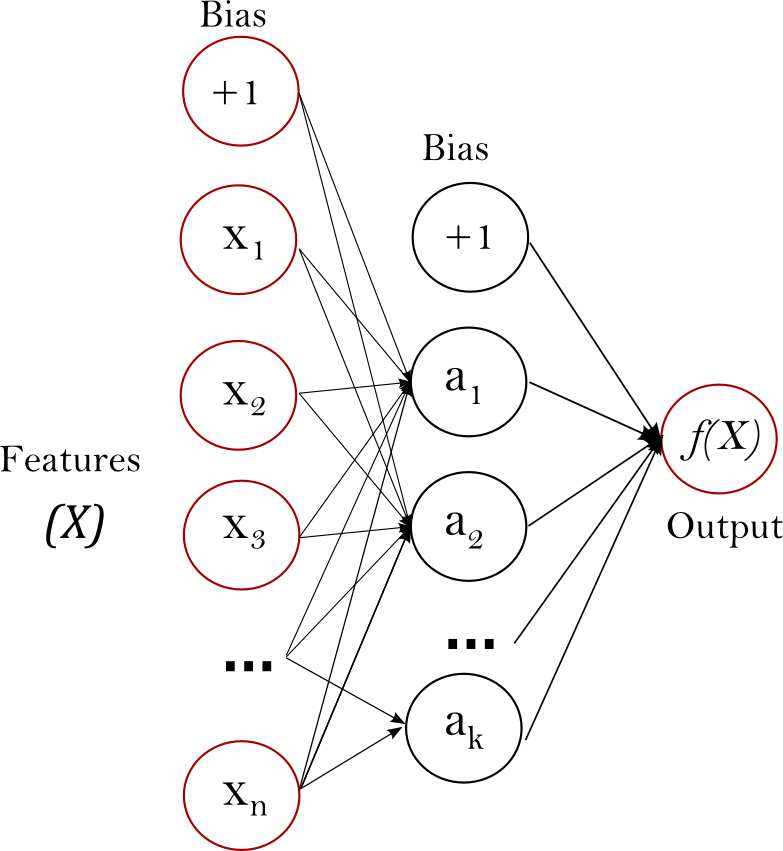
\includegraphics{../data/multilayerperceptron_network.png} The leftmost
layer, known as the input layer, consists of a set of "neurons"
\(\{x_i | x_1, x_2, ..., x_m\}\) representing the input features (e.g.,
weighted words). Each neuron in the hidden layer transforms the values
from the previous layer with a weighted linear summation
\(w_1x_1 + w_2x_2 + ... + w_mx_m\), followed by a non-linear activation
function \(g(\cdot):R \rightarrow R\) - like the logistic or hyperbolic
tan function. The output layer receives the values from the last hidden
layer and transforms them into output values.

    \begin{Verbatim}[commandchars=\\\{\}]
{\color{incolor}In [{\color{incolor}7}]:} \PY{n}{clf\PYZus{}nn} \PY{o}{=} \PY{n}{sklearn}\PY{o}{.}\PY{n}{neural\PYZus{}network}\PY{o}{.}\PY{n}{MLPClassifier}\PY{p}{(}\PY{p}{)}
        \PY{n}{clf\PYZus{}nn}\PY{o}{.}\PY{n}{fit}\PY{p}{(}\PY{n}{np}\PY{o}{.}\PY{n}{stack}\PY{p}{(}\PY{n}{train\PYZus{}redditDf}\PY{p}{[}\PY{l+s+s1}{\PYZsq{}}\PY{l+s+s1}{vect}\PY{l+s+s1}{\PYZsq{}}\PY{p}{]}\PY{p}{,} \PY{n}{axis}\PY{o}{=}\PY{l+m+mi}{0}\PY{p}{)}\PY{p}{,} \PY{n}{train\PYZus{}redditDf}\PY{p}{[}\PY{l+s+s1}{\PYZsq{}}\PY{l+s+s1}{category}\PY{l+s+s1}{\PYZsq{}}\PY{p}{]}\PY{p}{)}
\end{Verbatim}


    \begin{Verbatim}[commandchars=\\\{\}]

        ---------------------------------------------------------------------------

        NameError                                 Traceback (most recent call last)

        <ipython-input-7-241da2f91441> in <module>()
          1 clf\_nn = sklearn.neural\_network.MLPClassifier()
    ----> 2 clf\_nn.fit(np.stack(train\_redditDf['vect'], axis=0), train\_redditDf['category'])
    

        NameError: name 'train\_redditDf' is not defined

    \end{Verbatim}

    \begin{Verbatim}[commandchars=\\\{\}]
{\color{incolor}In [{\color{incolor}11}]:} \PY{n}{lucem\PYZus{}illud}\PY{o}{.}\PY{n}{evaluateClassifier}\PY{p}{(}\PY{n}{clf\PYZus{}nn}\PY{p}{,} \PY{n}{test\PYZus{}redditDf}\PY{p}{)}
\end{Verbatim}


\begin{Verbatim}[commandchars=\\\{\}]
{\color{outcolor}Out[{\color{outcolor}11}]:}                                                          AUC  \textbackslash{}
         Category                                                       
         Weeaboo Tales: stories about the extreme fans o{\ldots}  0.986301   
         Bad Roommates: Tales of Irritation                  0.983323   
         Relationships                                       0.959618   
         Tales From Tech Support                             0.995781   
         
                                                             Average\_Precision  \textbackslash{}
         Category                                                                
         Weeaboo Tales: stories about the extreme fans o{\ldots}           0.978872   
         Bad Roommates: Tales of Irritation                           0.932692   
         Relationships                                                0.923033   
         Tales From Tech Support                                      0.976190   
         
                                                             Error\_Rate  Precision  \textbackslash{}
         Category                                                                    
         Weeaboo Tales: stories about the extreme fans o{\ldots}    0.006270   1.000000   
         Bad Roommates: Tales of Irritation                    0.018809   0.941176   
         Relationships                                         0.025078   0.974684   
         Tales From Tech Support                               0.006270   0.976190   
         
                                                               Recall  
         Category                                                      
         Weeaboo Tales: stories about the extreme fans o{\ldots}  0.972603  
         Bad Roommates: Tales of Irritation                  0.987654  
         Relationships                                       0.927711  
         Tales From Tech Support                             1.000000  
\end{Verbatim}
            
    \begin{Verbatim}[commandchars=\\\{\}]
{\color{incolor}In [{\color{incolor}12}]:} \PY{n}{lucem\PYZus{}illud}\PY{o}{.}\PY{n}{plotConfusionMatrix}\PY{p}{(}\PY{n}{clf\PYZus{}nn}\PY{p}{,} \PY{n}{test\PYZus{}redditDf}\PY{p}{)}
\end{Verbatim}


    \begin{center}
    \adjustimage{max size={0.9\linewidth}{0.9\paperheight}}{output_232_0.png}
    \end{center}
    { \hspace*{\fill} \\}
    
    \begin{Verbatim}[commandchars=\\\{\}]
{\color{incolor}In [{\color{incolor}13}]:} \PY{n}{lucem\PYZus{}illud}\PY{o}{.}\PY{n}{plotregions}\PY{p}{(}\PY{n}{clf\PYZus{}nn}\PY{p}{,} \PY{n}{test\PYZus{}redditDf}\PY{p}{)}
\end{Verbatim}


    \begin{center}
    \adjustimage{max size={0.9\linewidth}{0.9\paperheight}}{output_233_0.png}
    \end{center}
    { \hspace*{\fill} \\}
    
    It performs very well.

    \subsection{\texorpdfstring{{\emph{Exercise
5}}}{Exercise 5}}\label{exercise-5}

In the cells immediately following, perform a neural network
classification and calculate relevant metrics (e.g., precision, recall,
the F-measure, and AUC). How does this classify relevant to
\emph{k}-nearest neighbor, Naive Bayes, logistic and decision-tree
approaches?

The neural net method for classification is less accurate in classifying
the documents as compared to the K-Nearest and Decision Tree classifier,
but only by approximately 3\%

    \begin{Verbatim}[commandchars=\\\{\}]
{\color{incolor}In [{\color{incolor}3}]:} \PY{n}{plos\PYZus{}df} \PY{o}{=} \PY{n}{pd}\PY{o}{.}\PY{n}{read\PYZus{}pickle}\PY{p}{(}\PY{l+s+s1}{\PYZsq{}}\PY{l+s+s1}{../6\PYZhy{}Classification/plos\PYZus{}classification.pk1}\PY{l+s+s1}{\PYZsq{}}\PY{p}{)}
        
        \PY{c+c1}{\PYZsh{}Changing the name of the journal title column to category so it works with the example code better}
        \PY{n}{plos\PYZus{}df}\PY{o}{.}\PY{n}{rename}\PY{p}{(}\PY{n}{columns}\PY{o}{=}\PY{p}{\PYZob{}}\PY{l+s+s1}{\PYZsq{}}\PY{l+s+s1}{Journal Title}\PY{l+s+s1}{\PYZsq{}}\PY{p}{:} \PY{l+s+s1}{\PYZsq{}}\PY{l+s+s1}{category}\PY{l+s+s1}{\PYZsq{}}\PY{p}{\PYZcb{}}\PY{p}{,} \PY{n}{inplace}\PY{o}{=}\PY{k+kc}{True}\PY{p}{)}
\end{Verbatim}


    \begin{Verbatim}[commandchars=\\\{\}]
{\color{incolor}In [{\color{incolor}4}]:} \PY{n}{plosTFVectorizer} \PY{o}{=} \PY{n}{sklearn}\PY{o}{.}\PY{n}{feature\PYZus{}extraction}\PY{o}{.}\PY{n}{text}\PY{o}{.}\PY{n}{TfidfVectorizer}\PY{p}{(}\PY{n}{max\PYZus{}df}\PY{o}{=}\PY{l+m+mf}{0.5}\PY{p}{,} \PY{n}{min\PYZus{}df}\PY{o}{=}\PY{l+m+mi}{3}\PY{p}{,} \PY{n}{stop\PYZus{}words}\PY{o}{=}\PY{l+s+s1}{\PYZsq{}}\PY{l+s+s1}{english}\PY{l+s+s1}{\PYZsq{}}\PY{p}{,} \PY{n}{norm}\PY{o}{=}\PY{l+s+s1}{\PYZsq{}}\PY{l+s+s1}{l2}\PY{l+s+s1}{\PYZsq{}}\PY{p}{)}
        \PY{n}{plosTFVects} \PY{o}{=} \PY{n}{plosTFVectorizer}\PY{o}{.}\PY{n}{fit\PYZus{}transform}\PY{p}{(}\PY{p}{[}\PY{l+s+s1}{\PYZsq{}}\PY{l+s+s1}{ }\PY{l+s+s1}{\PYZsq{}}\PY{o}{.}\PY{n}{join}\PY{p}{(}\PY{n}{l}\PY{p}{)} \PY{k}{for} \PY{n}{l} \PY{o+ow}{in} \PY{n}{plos\PYZus{}df}\PY{p}{[}\PY{l+s+s1}{\PYZsq{}}\PY{l+s+s1}{normalized\PYZus{}text}\PY{l+s+s1}{\PYZsq{}}\PY{p}{]}\PY{p}{]}\PY{p}{)}
        \PY{n}{plos\PYZus{}df}\PY{p}{[}\PY{l+s+s1}{\PYZsq{}}\PY{l+s+s1}{vect}\PY{l+s+s1}{\PYZsq{}}\PY{p}{]} \PY{o}{=} \PY{p}{[}\PY{n}{np}\PY{o}{.}\PY{n}{array}\PY{p}{(}\PY{n}{v}\PY{p}{)}\PY{o}{.}\PY{n}{flatten}\PY{p}{(}\PY{p}{)} \PY{k}{for} \PY{n}{v} \PY{o+ow}{in} \PY{n}{plosTFVects}\PY{o}{.}\PY{n}{todense}\PY{p}{(}\PY{p}{)}\PY{p}{]}
\end{Verbatim}


    \begin{Verbatim}[commandchars=\\\{\}]
{\color{incolor}In [{\color{incolor}5}]:} \PY{n}{holdBackFraction} \PY{o}{=} \PY{o}{.}\PY{l+m+mi}{2}
        \PY{n}{train\PYZus{}plos\PYZus{}df}\PY{p}{,} \PY{n}{test\PYZus{}plos\PYZus{}df} \PY{o}{=} \PY{n}{lucem\PYZus{}illud}\PY{o}{.}\PY{n}{trainTestSplit}\PY{p}{(}\PY{n}{plos\PYZus{}df}\PY{p}{,} \PY{n}{holdBackFraction}\PY{o}{=}\PY{n}{holdBackFraction}\PY{p}{)}
\end{Verbatim}


    \begin{Verbatim}[commandchars=\\\{\}]
{\color{incolor}In [{\color{incolor}6}]:} \PY{n}{clf\PYZus{}nn} \PY{o}{=} \PY{n}{sklearn}\PY{o}{.}\PY{n}{neural\PYZus{}network}\PY{o}{.}\PY{n}{MLPClassifier}\PY{p}{(}\PY{p}{)}
        \PY{n}{clf\PYZus{}nn}\PY{o}{.}\PY{n}{fit}\PY{p}{(}\PY{n}{np}\PY{o}{.}\PY{n}{stack}\PY{p}{(}\PY{n}{train\PYZus{}plos\PYZus{}df}\PY{p}{[}\PY{l+s+s1}{\PYZsq{}}\PY{l+s+s1}{vect}\PY{l+s+s1}{\PYZsq{}}\PY{p}{]}\PY{p}{,} \PY{n}{axis}\PY{o}{=}\PY{l+m+mi}{0}\PY{p}{)}\PY{p}{,} \PY{n}{train\PYZus{}plos\PYZus{}df}\PY{p}{[}\PY{l+s+s1}{\PYZsq{}}\PY{l+s+s1}{category}\PY{l+s+s1}{\PYZsq{}}\PY{p}{]}\PY{p}{)}
\end{Verbatim}


\begin{Verbatim}[commandchars=\\\{\}]
{\color{outcolor}Out[{\color{outcolor}6}]:} MLPClassifier(activation='relu', alpha=0.0001, batch\_size='auto', beta\_1=0.9,
               beta\_2=0.999, early\_stopping=False, epsilon=1e-08,
               hidden\_layer\_sizes=(100,), learning\_rate='constant',
               learning\_rate\_init=0.001, max\_iter=200, momentum=0.9,
               nesterovs\_momentum=True, power\_t=0.5, random\_state=None,
               shuffle=True, solver='adam', tol=0.0001, validation\_fraction=0.1,
               verbose=False, warm\_start=False)
\end{Verbatim}
            
    \begin{Verbatim}[commandchars=\\\{\}]
{\color{incolor}In [{\color{incolor}7}]:} \PY{n}{lucem\PYZus{}illud}\PY{o}{.}\PY{n}{evaluateClassifier}\PY{p}{(}\PY{n}{clf\PYZus{}nn}\PY{p}{,} \PY{n}{test\PYZus{}plos\PYZus{}df}\PY{p}{)}
\end{Verbatim}


    \begin{Verbatim}[commandchars=\\\{\}]
/software/Anaconda3-5.0.0.1-el7-x86\_64/lib/python3.6/site-packages/sklearn/metrics/classification.py:1135: UndefinedMetricWarning: Precision is ill-defined and being set to 0.0 due to no predicted samples.
  'precision', 'predicted', average, warn\_for)

    \end{Verbatim}

\begin{Verbatim}[commandchars=\\\{\}]
{\color{outcolor}Out[{\color{outcolor}7}]:}                                        AUC  Average\_Precision  Error\_Rate  \textbackslash{}
        Category                                                                    
        plos one                          0.513514           0.819095       0.180   
        none                              0.500000           0.040000       0.040   
        plos computational biology        0.500000           0.040000       0.040   
        plos neglected tropical diseases  0.500000           0.045000       0.045   
        plos pathogens                    0.497409           0.035000       0.040   
        plos medicine                     0.500000           0.005000       0.005   
        plos biology                      0.500000           0.005000       0.005   
        plos genetics                     0.500000           0.015000       0.015   
        
                                          Precision  Recall  
        Category                                             
        plos one                           0.819095     1.0  
        none                               0.000000     0.0  
        plos computational biology         0.000000     0.0  
        plos neglected tropical diseases   0.000000     0.0  
        plos pathogens                     0.000000     0.0  
        plos medicine                      0.000000     0.0  
        plos biology                       0.000000     0.0  
        plos genetics                      0.000000     0.0  
\end{Verbatim}
            
    \begin{Verbatim}[commandchars=\\\{\}]
{\color{incolor}In [{\color{incolor} }]:} \PY{n}{lucem\PYZus{}illud}\PY{o}{.}\PY{n}{plotConfusionMatrix}\PY{p}{(}\PY{n}{clf\PYZus{}nn}\PY{p}{,} \PY{n}{test\PYZus{}plos\PYZus{}df}\PY{p}{)}
\end{Verbatim}


    \begin{center}
    \adjustimage{max size={0.9\linewidth}{0.9\paperheight}}{output_241_0.png}
    \end{center}
    { \hspace*{\fill} \\}
    
    \begin{Verbatim}[commandchars=\\\{\}]
{\color{incolor}In [{\color{incolor} }]:} \PY{n}{lucem\PYZus{}illud}\PY{o}{.}\PY{n}{plotregions}\PY{p}{(}\PY{n}{clf\PYZus{}nn}\PY{p}{,} \PY{n}{test\PYZus{}plos\PYZus{}df}\PY{p}{)}
\end{Verbatim}



    % Add a bibliography block to the postdoc
    
    
    
    \end{document}
